\documentclass[11pt]{article}
	\usepackage[utf8]{inputenc}
    \usepackage[breakable]{tcolorbox}
    \usepackage{parskip} % Stop auto-indenting (to mimic markdown behaviour)
    
    \usepackage{iftex}
    \ifPDFTeX
    	\usepackage[T1]{fontenc}
    	\usepackage{mathpazo}
    \else
    	\usepackage{fontspec}
    \fi

    % Basic figure setup, for now with no caption control since it's done
    % automatically by Pandoc (which extracts ![](path) syntax from Markdown).
    \usepackage{graphicx}
    % Maintain compatibility with old templates. Remove in nbconvert 6.0
    \let\Oldincludegraphics\includegraphics
    % Ensure that by default, figures have no caption (until we provide a
    % proper Figure object with a Caption API and a way to capture that
    % in the conversion process - todo).
    \usepackage{caption}
    \DeclareCaptionFormat{nocaption}{}
    \captionsetup{format=nocaption,aboveskip=0pt,belowskip=0pt}

    \usepackage[Export]{adjustbox} % Used to constrain images to a maximum size
    \adjustboxset{max size={0.9\linewidth}{0.9\paperheight}}
    \usepackage{float}
    \floatplacement{figure}{H} % forces figures to be placed at the correct location
    \usepackage{xcolor} % Allow colors to be defined
    \usepackage{enumerate} % Needed for markdown enumerations to work
    \usepackage{geometry} % Used to adjust the document margins
    \usepackage{amsmath} % Equations
    \usepackage{amssymb} % Equations
    \usepackage{textcomp} % defines textquotesingle
    % Hack from http://tex.stackexchange.com/a/47451/13684:
    \AtBeginDocument{%
        \def\PYZsq{\textquotesingle}% Upright quotes in Pygmentized code
    }
    \usepackage{upquote} % Upright quotes for verbatim code
    \usepackage{eurosym} % defines \euro
    \usepackage[mathletters]{ucs} % Extended unicode (utf-8) support
    \usepackage{fancyvrb} % verbatim replacement that allows latex
    \usepackage{grffile} % extends the file name processing of package graphics 
                         % to support a larger range
    \makeatletter % fix for grffile with XeLaTeX
    \def\Gread@@xetex#1{%
      \IfFileExists{"\Gin@base".bb}%
      {\Gread@eps{\Gin@base.bb}}%
      {\Gread@@xetex@aux#1}%
    }
    \makeatother

    % The hyperref package gives us a pdf with properly built
    % internal navigation ('pdf bookmarks' for the table of contents,
    % internal cross-reference links, web links for URLs, etc.)
    \usepackage{hyperref}
    % The default LaTeX title has an obnoxious amount of whitespace. By default,
    % titling removes some of it. It also provides customization options.
    \usepackage{titling}
    \usepackage{longtable} % longtable support required by pandoc >1.10
    \usepackage{booktabs}  % table support for pandoc > 1.12.2
    \usepackage[inline]{enumitem} % IRkernel/repr support (it uses the enumerate* environment)
    \usepackage[normalem]{ulem} % ulem is needed to support strikethroughs (\sout)
                                % normalem makes italics be italics, not underlines
    \usepackage{mathrsfs}
    

    
    % Colors for the hyperref package
    \definecolor{urlcolor}{rgb}{0,.145,.698}
    \definecolor{linkcolor}{rgb}{.71,0.21,0.01}
    \definecolor{citecolor}{rgb}{.12,.54,.11}

    % ANSI colors
    \definecolor{ansi-black}{HTML}{3E424D}
    \definecolor{ansi-black-intense}{HTML}{282C36}
    \definecolor{ansi-red}{HTML}{E75C58}
    \definecolor{ansi-red-intense}{HTML}{B22B31}
    \definecolor{ansi-green}{HTML}{00A250}
    \definecolor{ansi-green-intense}{HTML}{007427}
    \definecolor{ansi-yellow}{HTML}{DDB62B}
    \definecolor{ansi-yellow-intense}{HTML}{B27D12}
    \definecolor{ansi-blue}{HTML}{208FFB}
    \definecolor{ansi-blue-intense}{HTML}{0065CA}
    \definecolor{ansi-magenta}{HTML}{D160C4}
    \definecolor{ansi-magenta-intense}{HTML}{A03196}
    \definecolor{ansi-cyan}{HTML}{60C6C8}
    \definecolor{ansi-cyan-intense}{HTML}{258F8F}
    \definecolor{ansi-white}{HTML}{C5C1B4}
    \definecolor{ansi-white-intense}{HTML}{A1A6B2}
    \definecolor{ansi-default-inverse-fg}{HTML}{FFFFFF}
    \definecolor{ansi-default-inverse-bg}{HTML}{000000}

    % commands and environments needed by pandoc snippets
    % extracted from the output of `pandoc -s`
    \providecommand{\tightlist}{%
      \setlength{\itemsep}{0pt}\setlength{\parskip}{0pt}}
    \DefineVerbatimEnvironment{Highlighting}{Verbatim}{commandchars=\\\{\}}
    % Add ',fontsize=\small' for more characters per line
    \newenvironment{Shaded}{}{}
    \newcommand{\KeywordTok}[1]{\textcolor[rgb]{0.00,0.44,0.13}{\textbf{{#1}}}}
    \newcommand{\DataTypeTok}[1]{\textcolor[rgb]{0.56,0.13,0.00}{{#1}}}
    \newcommand{\DecValTok}[1]{\textcolor[rgb]{0.25,0.63,0.44}{{#1}}}
    \newcommand{\BaseNTok}[1]{\textcolor[rgb]{0.25,0.63,0.44}{{#1}}}
    \newcommand{\FloatTok}[1]{\textcolor[rgb]{0.25,0.63,0.44}{{#1}}}
    \newcommand{\CharTok}[1]{\textcolor[rgb]{0.25,0.44,0.63}{{#1}}}
    \newcommand{\StringTok}[1]{\textcolor[rgb]{0.25,0.44,0.63}{{#1}}}
    \newcommand{\CommentTok}[1]{\textcolor[rgb]{0.38,0.63,0.69}{\textit{{#1}}}}
    \newcommand{\OtherTok}[1]{\textcolor[rgb]{0.00,0.44,0.13}{{#1}}}
    \newcommand{\AlertTok}[1]{\textcolor[rgb]{1.00,0.00,0.00}{\textbf{{#1}}}}
    \newcommand{\FunctionTok}[1]{\textcolor[rgb]{0.02,0.16,0.49}{{#1}}}
    \newcommand{\RegionMarkerTok}[1]{{#1}}
    \newcommand{\ErrorTok}[1]{\textcolor[rgb]{1.00,0.00,0.00}{\textbf{{#1}}}}
    \newcommand{\NormalTok}[1]{{#1}}
    
    % Additional commands for more recent versions of Pandoc
    \newcommand{\ConstantTok}[1]{\textcolor[rgb]{0.53,0.00,0.00}{{#1}}}
    \newcommand{\SpecialCharTok}[1]{\textcolor[rgb]{0.25,0.44,0.63}{{#1}}}
    \newcommand{\VerbatimStringTok}[1]{\textcolor[rgb]{0.25,0.44,0.63}{{#1}}}
    \newcommand{\SpecialStringTok}[1]{\textcolor[rgb]{0.73,0.40,0.53}{{#1}}}
    \newcommand{\ImportTok}[1]{{#1}}
    \newcommand{\DocumentationTok}[1]{\textcolor[rgb]{0.73,0.13,0.13}{\textit{{#1}}}}
    \newcommand{\AnnotationTok}[1]{\textcolor[rgb]{0.38,0.63,0.69}{\textbf{\textit{{#1}}}}}
    \newcommand{\CommentVarTok}[1]{\textcolor[rgb]{0.38,0.63,0.69}{\textbf{\textit{{#1}}}}}
    \newcommand{\VariableTok}[1]{\textcolor[rgb]{0.10,0.09,0.49}{{#1}}}
    \newcommand{\ControlFlowTok}[1]{\textcolor[rgb]{0.00,0.44,0.13}{\textbf{{#1}}}}
    \newcommand{\OperatorTok}[1]{\textcolor[rgb]{0.40,0.40,0.40}{{#1}}}
    \newcommand{\BuiltInTok}[1]{{#1}}
    \newcommand{\ExtensionTok}[1]{{#1}}
    \newcommand{\PreprocessorTok}[1]{\textcolor[rgb]{0.74,0.48,0.00}{{#1}}}
    \newcommand{\AttributeTok}[1]{\textcolor[rgb]{0.49,0.56,0.16}{{#1}}}
    \newcommand{\InformationTok}[1]{\textcolor[rgb]{0.38,0.63,0.69}{\textbf{\textit{{#1}}}}}
    \newcommand{\WarningTok}[1]{\textcolor[rgb]{0.38,0.63,0.69}{\textbf{\textit{{#1}}}}}
    
    
    % Define a nice break command that doesn't care if a line doesn't already
    % exist.
    \def\br{\hspace*{\fill} \\* }
    % Math Jax compatibility definitions
    \def\gt{>}
    \def\lt{<}
    \let\Oldtex\TeX
    \let\Oldlatex\LaTeX
    \renewcommand{\TeX}{\textrm{\Oldtex}}
    \renewcommand{\LaTeX}{\textrm{\Oldlatex}}
    % Document parameters
    % Document title
    \title{Projet Formule 1}
    
    
    
    
    
% Pygments definitions
\makeatletter
\def\PY@reset{\let\PY@it=\relax \let\PY@bf=\relax%
    \let\PY@ul=\relax \let\PY@tc=\relax%
    \let\PY@bc=\relax \let\PY@ff=\relax}
\def\PY@tok#1{\csname PY@tok@#1\endcsname}
\def\PY@toks#1+{\ifx\relax#1\empty\else%
    \PY@tok{#1}\expandafter\PY@toks\fi}
\def\PY@do#1{\PY@bc{\PY@tc{\PY@ul{%
    \PY@it{\PY@bf{\PY@ff{#1}}}}}}}
\def\PY#1#2{\PY@reset\PY@toks#1+\relax+\PY@do{#2}}

\expandafter\def\csname PY@tok@gd\endcsname{\def\PY@tc##1{\textcolor[rgb]{0.63,0.00,0.00}{##1}}}
\expandafter\def\csname PY@tok@gu\endcsname{\let\PY@bf=\textbf\def\PY@tc##1{\textcolor[rgb]{0.50,0.00,0.50}{##1}}}
\expandafter\def\csname PY@tok@gt\endcsname{\def\PY@tc##1{\textcolor[rgb]{0.00,0.27,0.87}{##1}}}
\expandafter\def\csname PY@tok@gs\endcsname{\let\PY@bf=\textbf}
\expandafter\def\csname PY@tok@gr\endcsname{\def\PY@tc##1{\textcolor[rgb]{1.00,0.00,0.00}{##1}}}
\expandafter\def\csname PY@tok@cm\endcsname{\let\PY@it=\textit\def\PY@tc##1{\textcolor[rgb]{0.25,0.50,0.50}{##1}}}
\expandafter\def\csname PY@tok@vg\endcsname{\def\PY@tc##1{\textcolor[rgb]{0.10,0.09,0.49}{##1}}}
\expandafter\def\csname PY@tok@vi\endcsname{\def\PY@tc##1{\textcolor[rgb]{0.10,0.09,0.49}{##1}}}
\expandafter\def\csname PY@tok@vm\endcsname{\def\PY@tc##1{\textcolor[rgb]{0.10,0.09,0.49}{##1}}}
\expandafter\def\csname PY@tok@mh\endcsname{\def\PY@tc##1{\textcolor[rgb]{0.40,0.40,0.40}{##1}}}
\expandafter\def\csname PY@tok@cs\endcsname{\let\PY@it=\textit\def\PY@tc##1{\textcolor[rgb]{0.25,0.50,0.50}{##1}}}
\expandafter\def\csname PY@tok@ge\endcsname{\let\PY@it=\textit}
\expandafter\def\csname PY@tok@vc\endcsname{\def\PY@tc##1{\textcolor[rgb]{0.10,0.09,0.49}{##1}}}
\expandafter\def\csname PY@tok@il\endcsname{\def\PY@tc##1{\textcolor[rgb]{0.40,0.40,0.40}{##1}}}
\expandafter\def\csname PY@tok@go\endcsname{\def\PY@tc##1{\textcolor[rgb]{0.53,0.53,0.53}{##1}}}
\expandafter\def\csname PY@tok@cp\endcsname{\def\PY@tc##1{\textcolor[rgb]{0.74,0.48,0.00}{##1}}}
\expandafter\def\csname PY@tok@gi\endcsname{\def\PY@tc##1{\textcolor[rgb]{0.00,0.63,0.00}{##1}}}
\expandafter\def\csname PY@tok@gh\endcsname{\let\PY@bf=\textbf\def\PY@tc##1{\textcolor[rgb]{0.00,0.00,0.50}{##1}}}
\expandafter\def\csname PY@tok@ni\endcsname{\let\PY@bf=\textbf\def\PY@tc##1{\textcolor[rgb]{0.60,0.60,0.60}{##1}}}
\expandafter\def\csname PY@tok@nl\endcsname{\def\PY@tc##1{\textcolor[rgb]{0.63,0.63,0.00}{##1}}}
\expandafter\def\csname PY@tok@nn\endcsname{\let\PY@bf=\textbf\def\PY@tc##1{\textcolor[rgb]{0.00,0.00,1.00}{##1}}}
\expandafter\def\csname PY@tok@no\endcsname{\def\PY@tc##1{\textcolor[rgb]{0.53,0.00,0.00}{##1}}}
\expandafter\def\csname PY@tok@na\endcsname{\def\PY@tc##1{\textcolor[rgb]{0.49,0.56,0.16}{##1}}}
\expandafter\def\csname PY@tok@nb\endcsname{\def\PY@tc##1{\textcolor[rgb]{0.00,0.50,0.00}{##1}}}
\expandafter\def\csname PY@tok@nc\endcsname{\let\PY@bf=\textbf\def\PY@tc##1{\textcolor[rgb]{0.00,0.00,1.00}{##1}}}
\expandafter\def\csname PY@tok@nd\endcsname{\def\PY@tc##1{\textcolor[rgb]{0.67,0.13,1.00}{##1}}}
\expandafter\def\csname PY@tok@ne\endcsname{\let\PY@bf=\textbf\def\PY@tc##1{\textcolor[rgb]{0.82,0.25,0.23}{##1}}}
\expandafter\def\csname PY@tok@nf\endcsname{\def\PY@tc##1{\textcolor[rgb]{0.00,0.00,1.00}{##1}}}
\expandafter\def\csname PY@tok@si\endcsname{\let\PY@bf=\textbf\def\PY@tc##1{\textcolor[rgb]{0.73,0.40,0.53}{##1}}}
\expandafter\def\csname PY@tok@s2\endcsname{\def\PY@tc##1{\textcolor[rgb]{0.73,0.13,0.13}{##1}}}
\expandafter\def\csname PY@tok@nt\endcsname{\let\PY@bf=\textbf\def\PY@tc##1{\textcolor[rgb]{0.00,0.50,0.00}{##1}}}
\expandafter\def\csname PY@tok@nv\endcsname{\def\PY@tc##1{\textcolor[rgb]{0.10,0.09,0.49}{##1}}}
\expandafter\def\csname PY@tok@s1\endcsname{\def\PY@tc##1{\textcolor[rgb]{0.73,0.13,0.13}{##1}}}
\expandafter\def\csname PY@tok@dl\endcsname{\def\PY@tc##1{\textcolor[rgb]{0.73,0.13,0.13}{##1}}}
\expandafter\def\csname PY@tok@ch\endcsname{\let\PY@it=\textit\def\PY@tc##1{\textcolor[rgb]{0.25,0.50,0.50}{##1}}}
\expandafter\def\csname PY@tok@m\endcsname{\def\PY@tc##1{\textcolor[rgb]{0.40,0.40,0.40}{##1}}}
\expandafter\def\csname PY@tok@gp\endcsname{\let\PY@bf=\textbf\def\PY@tc##1{\textcolor[rgb]{0.00,0.00,0.50}{##1}}}
\expandafter\def\csname PY@tok@sh\endcsname{\def\PY@tc##1{\textcolor[rgb]{0.73,0.13,0.13}{##1}}}
\expandafter\def\csname PY@tok@ow\endcsname{\let\PY@bf=\textbf\def\PY@tc##1{\textcolor[rgb]{0.67,0.13,1.00}{##1}}}
\expandafter\def\csname PY@tok@sx\endcsname{\def\PY@tc##1{\textcolor[rgb]{0.00,0.50,0.00}{##1}}}
\expandafter\def\csname PY@tok@bp\endcsname{\def\PY@tc##1{\textcolor[rgb]{0.00,0.50,0.00}{##1}}}
\expandafter\def\csname PY@tok@c1\endcsname{\let\PY@it=\textit\def\PY@tc##1{\textcolor[rgb]{0.25,0.50,0.50}{##1}}}
\expandafter\def\csname PY@tok@fm\endcsname{\def\PY@tc##1{\textcolor[rgb]{0.00,0.00,1.00}{##1}}}
\expandafter\def\csname PY@tok@o\endcsname{\def\PY@tc##1{\textcolor[rgb]{0.40,0.40,0.40}{##1}}}
\expandafter\def\csname PY@tok@kc\endcsname{\let\PY@bf=\textbf\def\PY@tc##1{\textcolor[rgb]{0.00,0.50,0.00}{##1}}}
\expandafter\def\csname PY@tok@c\endcsname{\let\PY@it=\textit\def\PY@tc##1{\textcolor[rgb]{0.25,0.50,0.50}{##1}}}
\expandafter\def\csname PY@tok@mf\endcsname{\def\PY@tc##1{\textcolor[rgb]{0.40,0.40,0.40}{##1}}}
\expandafter\def\csname PY@tok@err\endcsname{\def\PY@bc##1{\setlength{\fboxsep}{0pt}\fcolorbox[rgb]{1.00,0.00,0.00}{1,1,1}{\strut ##1}}}
\expandafter\def\csname PY@tok@mb\endcsname{\def\PY@tc##1{\textcolor[rgb]{0.40,0.40,0.40}{##1}}}
\expandafter\def\csname PY@tok@ss\endcsname{\def\PY@tc##1{\textcolor[rgb]{0.10,0.09,0.49}{##1}}}
\expandafter\def\csname PY@tok@sr\endcsname{\def\PY@tc##1{\textcolor[rgb]{0.73,0.40,0.53}{##1}}}
\expandafter\def\csname PY@tok@mo\endcsname{\def\PY@tc##1{\textcolor[rgb]{0.40,0.40,0.40}{##1}}}
\expandafter\def\csname PY@tok@kd\endcsname{\let\PY@bf=\textbf\def\PY@tc##1{\textcolor[rgb]{0.00,0.50,0.00}{##1}}}
\expandafter\def\csname PY@tok@mi\endcsname{\def\PY@tc##1{\textcolor[rgb]{0.40,0.40,0.40}{##1}}}
\expandafter\def\csname PY@tok@kn\endcsname{\let\PY@bf=\textbf\def\PY@tc##1{\textcolor[rgb]{0.00,0.50,0.00}{##1}}}
\expandafter\def\csname PY@tok@cpf\endcsname{\let\PY@it=\textit\def\PY@tc##1{\textcolor[rgb]{0.25,0.50,0.50}{##1}}}
\expandafter\def\csname PY@tok@kr\endcsname{\let\PY@bf=\textbf\def\PY@tc##1{\textcolor[rgb]{0.00,0.50,0.00}{##1}}}
\expandafter\def\csname PY@tok@s\endcsname{\def\PY@tc##1{\textcolor[rgb]{0.73,0.13,0.13}{##1}}}
\expandafter\def\csname PY@tok@kp\endcsname{\def\PY@tc##1{\textcolor[rgb]{0.00,0.50,0.00}{##1}}}
\expandafter\def\csname PY@tok@w\endcsname{\def\PY@tc##1{\textcolor[rgb]{0.73,0.73,0.73}{##1}}}
\expandafter\def\csname PY@tok@kt\endcsname{\def\PY@tc##1{\textcolor[rgb]{0.69,0.00,0.25}{##1}}}
\expandafter\def\csname PY@tok@sc\endcsname{\def\PY@tc##1{\textcolor[rgb]{0.73,0.13,0.13}{##1}}}
\expandafter\def\csname PY@tok@sb\endcsname{\def\PY@tc##1{\textcolor[rgb]{0.73,0.13,0.13}{##1}}}
\expandafter\def\csname PY@tok@sa\endcsname{\def\PY@tc##1{\textcolor[rgb]{0.73,0.13,0.13}{##1}}}
\expandafter\def\csname PY@tok@k\endcsname{\let\PY@bf=\textbf\def\PY@tc##1{\textcolor[rgb]{0.00,0.50,0.00}{##1}}}
\expandafter\def\csname PY@tok@se\endcsname{\let\PY@bf=\textbf\def\PY@tc##1{\textcolor[rgb]{0.73,0.40,0.13}{##1}}}
\expandafter\def\csname PY@tok@sd\endcsname{\let\PY@it=\textit\def\PY@tc##1{\textcolor[rgb]{0.73,0.13,0.13}{##1}}}

\def\PYZbs{\char`\\}
\def\PYZus{\char`\_}
\def\PYZob{\char`\{}
\def\PYZcb{\char`\}}
\def\PYZca{\char`\^}
\def\PYZam{\char`\&}
\def\PYZlt{\char`\<}
\def\PYZgt{\char`\>}
\def\PYZsh{\char`\#}
\def\PYZpc{\char`\%}
\def\PYZdl{\char`\$}
\def\PYZhy{\char`\-}
\def\PYZsq{\char`\'}
\def\PYZdq{\char`\"}
\def\PYZti{\char`\~}
% for compatibility with earlier versions
\def\PYZat{@}
\def\PYZlb{[}
\def\PYZrb{]}
\makeatother


    % For linebreaks inside Verbatim environment from package fancyvrb. 
    \makeatletter
        \newbox\Wrappedcontinuationbox 
        \newbox\Wrappedvisiblespacebox 
        \newcommand*\Wrappedvisiblespace {\textcolor{red}{\textvisiblespace}} 
        \newcommand*\Wrappedcontinuationsymbol {\textcolor{red}{\llap{\tiny$\m@th\hookrightarrow$}}} 
        \newcommand*\Wrappedcontinuationindent {3ex } 
        \newcommand*\Wrappedafterbreak {\kern\Wrappedcontinuationindent\copy\Wrappedcontinuationbox} 
        % Take advantage of the already applied Pygments mark-up to insert 
        % potential linebreaks for TeX processing. 
        %        {, <, #, %, $, ' and ": go to next line. 
        %        _, }, ^, &, >, - and ~: stay at end of broken line. 
        % Use of \textquotesingle for straight quote. 
        \newcommand*\Wrappedbreaksatspecials {% 
            \def\PYGZus{\discretionary{\char`\_}{\Wrappedafterbreak}{\char`\_}}% 
            \def\PYGZob{\discretionary{}{\Wrappedafterbreak\char`\{}{\char`\{}}% 
            \def\PYGZcb{\discretionary{\char`\}}{\Wrappedafterbreak}{\char`\}}}% 
            \def\PYGZca{\discretionary{\char`\^}{\Wrappedafterbreak}{\char`\^}}% 
            \def\PYGZam{\discretionary{\char`\&}{\Wrappedafterbreak}{\char`\&}}% 
            \def\PYGZlt{\discretionary{}{\Wrappedafterbreak\char`\<}{\char`\<}}% 
            \def\PYGZgt{\discretionary{\char`\>}{\Wrappedafterbreak}{\char`\>}}% 
            \def\PYGZsh{\discretionary{}{\Wrappedafterbreak\char`\#}{\char`\#}}% 
            \def\PYGZpc{\discretionary{}{\Wrappedafterbreak\char`\%}{\char`\%}}% 
            \def\PYGZdl{\discretionary{}{\Wrappedafterbreak\char`\$}{\char`\$}}% 
            \def\PYGZhy{\discretionary{\char`\-}{\Wrappedafterbreak}{\char`\-}}% 
            \def\PYGZsq{\discretionary{}{\Wrappedafterbreak\textquotesingle}{\textquotesingle}}% 
            \def\PYGZdq{\discretionary{}{\Wrappedafterbreak\char`\"}{\char`\"}}% 
            \def\PYGZti{\discretionary{\char`\~}{\Wrappedafterbreak}{\char`\~}}% 
        } 
        % Some characters . , ; ? ! / are not pygmentized. 
        % This macro makes them "active" and they will insert potential linebreaks 
        \newcommand*\Wrappedbreaksatpunct {% 
            \lccode`\~`\.\lowercase{\def~}{\discretionary{\hbox{\char`\.}}{\Wrappedafterbreak}{\hbox{\char`\.}}}% 
            \lccode`\~`\,\lowercase{\def~}{\discretionary{\hbox{\char`\,}}{\Wrappedafterbreak}{\hbox{\char`\,}}}% 
            \lccode`\~`\;\lowercase{\def~}{\discretionary{\hbox{\char`\;}}{\Wrappedafterbreak}{\hbox{\char`\;}}}% 
            \lccode`\~`\:\lowercase{\def~}{\discretionary{\hbox{\char`\:}}{\Wrappedafterbreak}{\hbox{\char`\:}}}% 
            \lccode`\~`\?\lowercase{\def~}{\discretionary{\hbox{\char`\?}}{\Wrappedafterbreak}{\hbox{\char`\?}}}% 
            \lccode`\~`\!\lowercase{\def~}{\discretionary{\hbox{\char`\!}}{\Wrappedafterbreak}{\hbox{\char`\!}}}% 
            \lccode`\~`\/\lowercase{\def~}{\discretionary{\hbox{\char`\/}}{\Wrappedafterbreak}{\hbox{\char`\/}}}% 
            \catcode`\.\active
            \catcode`\,\active 
            \catcode`\;\active
            \catcode`\:\active
            \catcode`\?\active
            \catcode`\!\active
            \catcode`\/\active 
            \lccode`\~`\~ 	
        }
    \makeatother

    \let\OriginalVerbatim=\Verbatim
    \makeatletter
    \renewcommand{\Verbatim}[1][1]{%
        %\parskip\z@skip
        \sbox\Wrappedcontinuationbox {\Wrappedcontinuationsymbol}%
        \sbox\Wrappedvisiblespacebox {\FV@SetupFont\Wrappedvisiblespace}%
        \def\FancyVerbFormatLine ##1{\hsize\linewidth
            \vtop{\raggedright\hyphenpenalty\z@\exhyphenpenalty\z@
                \doublehyphendemerits\z@\finalhyphendemerits\z@
                \strut ##1\strut}%
        }%
        % If the linebreak is at a space, the latter will be displayed as visible
        % space at end of first line, and a continuation symbol starts next line.
        % Stretch/shrink are however usually zero for typewriter font.
        \def\FV@Space {%
            \nobreak\hskip\z@ plus\fontdimen3\font minus\fontdimen4\font
            \discretionary{\copy\Wrappedvisiblespacebox}{\Wrappedafterbreak}
            {\kern\fontdimen2\font}%
        }%
        
        % Allow breaks at special characters using \PYG... macros.
        \Wrappedbreaksatspecials
        % Breaks at punctuation characters . , ; ? ! and / need catcode=\active 	
        \OriginalVerbatim[#1,codes*=\Wrappedbreaksatpunct]%
    }
    \makeatother

    % Exact colors from NB
    \definecolor{incolor}{HTML}{303F9F}
    \definecolor{outcolor}{HTML}{D84315}
    \definecolor{cellborder}{HTML}{CFCFCF}
    \definecolor{cellbackground}{HTML}{F7F7F7}
    
    % prompt
    \makeatletter
    \newcommand{\boxspacing}{\kern\kvtcb@left@rule\kern\kvtcb@boxsep}
    \makeatother
    \newcommand{\prompt}[4]{
        \ttfamily\llap{{\color{#2}[#3]:\hspace{3pt}#4}}\vspace{-\baselineskip}
    }
    

    
    % Prevent overflowing lines due to hard-to-break entities
    \sloppy 
    % Setup hyperref package
    \hypersetup{
      breaklinks=true,  % so long urls are correctly broken across lines
      colorlinks=true,
      urlcolor=urlcolor,
      linkcolor=linkcolor,
      citecolor=citecolor,
      }
    % Slightly bigger margins than the latex defaults
    
    \geometry{verbose,tmargin=1in,bmargin=1in,lmargin=1in,rmargin=1in}
    
    

\begin{document}
    
    \maketitle
    
    

    
    \hypertarget{projet-analyse-de-donnuxe9es-stratuxe8ge-virtuel-de-formule-1}{%
\section{Projet Analyse de Données : Stratège virtuel de Formule
1}\label{projet-analyse-de-donnuxe9es-stratuxe8ge-virtuel-de-formule-1}}

Ce projet porte sur l'étude et l'analyse des résultats et de données de
toutes les courses de Formule 1 qui se sont déroulées de 1950 à 2018. En
Formule 1, de nombreux facteurs sont clés dans la route vers la victoire
d'un Grand Prix. On retrouve entre autres :

\begin{itemize}
\item La performance de la voiture

\item Le talent du pilote

\item La position sur la grille (déterminée par une séance de qualification)

\item La gestion de l'essence

\item La gestion de l'usure des pneus et l'utilisation astucieuse d'arrêts au
stand

\item La réactivité aux évènements de course comme la tombée de pluie, les
accidents sur piste
\end{itemize}


Dans ce projet, nous allons, entre autres, tenter de prédire la position
à l'arrivée d'un pilote, ou bien essayer de déterminer à quel moment de
la course un pilote a réalisé un arrêt au stand.

\begin{figure}
\centering
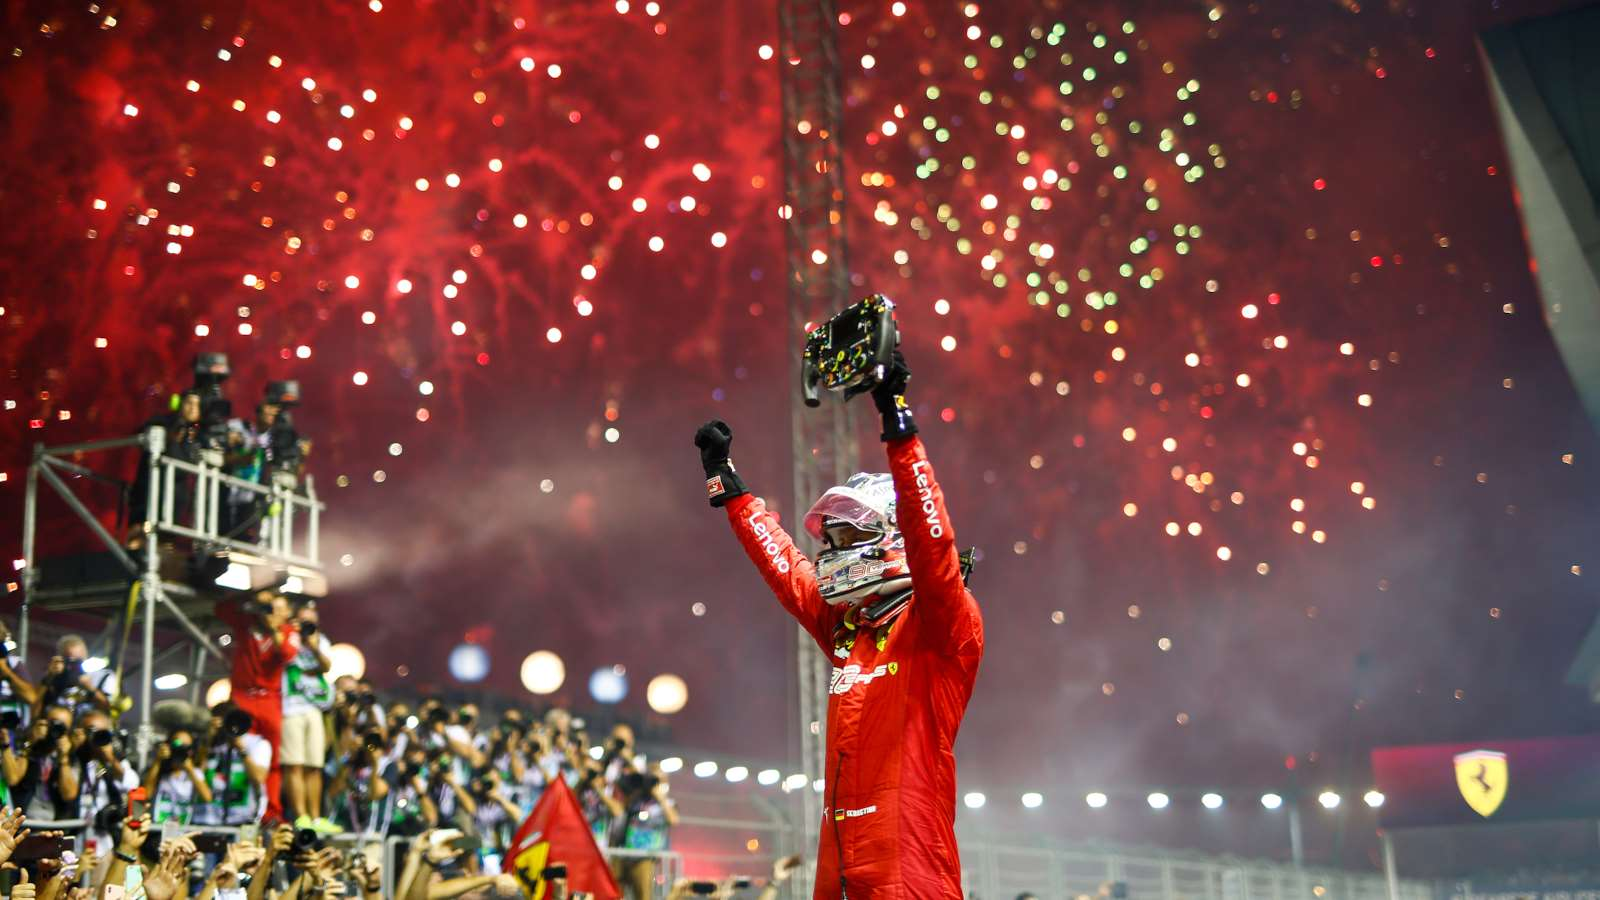
\includegraphics{vettel.jpg}
\caption{vettel.jpg}
\end{figure}

    On importe les librairies utiles pour ce projet.

    \begin{tcolorbox}[breakable, size=fbox, boxrule=1pt, pad at break*=1mm,colback=cellbackground, colframe=cellborder]
\prompt{In}{incolor}{364}{\boxspacing}
\begin{Verbatim}[commandchars=\\\{\}]
\PY{k+kn}{import} \PY{n+nn}{tensorflow} \PY{k+kn}{as} \PY{n+nn}{tf}
\PY{k+kn}{from} \PY{n+nn}{tensorflow} \PY{k+kn}{import} \PY{n}{keras}

\PY{k+kn}{import} \PY{n+nn}{os}
\PY{k+kn}{import} \PY{n+nn}{tempfile}

\PY{k+kn}{import} \PY{n+nn}{pandas} \PY{k+kn}{as} \PY{n+nn}{pd}
\PY{k+kn}{import} \PY{n+nn}{numpy} \PY{k+kn}{as} \PY{n+nn}{np}
\PY{k+kn}{import} \PY{n+nn}{matplotlib} \PY{k+kn}{as} \PY{n+nn}{mpl}
\PY{k+kn}{import} \PY{n+nn}{matplotlib.pyplot} \PY{k+kn}{as} \PY{n+nn}{plt}
\PY{k+kn}{import} \PY{n+nn}{seaborn} \PY{k+kn}{as} \PY{n+nn}{sns}
\PY{k+kn}{import} \PY{n+nn}{time}
\PY{k+kn}{import} \PY{n+nn}{sklearn}
\PY{k+kn}{from} \PY{n+nn}{sklearn.metrics} \PY{k+kn}{import} \PY{n}{confusion\PYZus{}matrix}
\PY{k+kn}{from} \PY{n+nn}{sklearn.model\PYZus{}selection} \PY{k+kn}{import} \PY{n}{train\PYZus{}test\PYZus{}split}
\PY{k+kn}{from} \PY{n+nn}{sklearn.preprocessing} \PY{k+kn}{import} \PY{n}{StandardScaler}
\PY{k+kn}{from} \PY{n+nn}{sklearn.linear\PYZus{}model} \PY{k+kn}{import} \PY{n}{LinearRegression}
\PY{k+kn}{from} \PY{n+nn}{sklearn} \PY{k+kn}{import} \PY{n}{metrics}
\PY{k+kn}{import} \PY{n+nn}{scikitplot} \PY{k+kn}{as} \PY{n+nn}{skplt}

\PY{n}{sns}\PY{o}{.}\PY{n}{set}\PY{p}{(}\PY{p}{)}
\PY{n}{mpl}\PY{o}{.}\PY{n}{rcParams}\PY{p}{[}\PY{l+s+s1}{\PYZsq{}}\PY{l+s+s1}{figure.figsize}\PY{l+s+s1}{\PYZsq{}}\PY{p}{]} \PY{o}{=} \PY{p}{(}\PY{l+m+mi}{12}\PY{p}{,} \PY{l+m+mi}{10}\PY{p}{)}
\PY{n}{colors} \PY{o}{=} \PY{n}{plt}\PY{o}{.}\PY{n}{rcParams}\PY{p}{[}\PY{l+s+s1}{\PYZsq{}}\PY{l+s+s1}{axes.prop\PYZus{}cycle}\PY{l+s+s1}{\PYZsq{}}\PY{p}{]}\PY{o}{.}\PY{n}{by\PYZus{}key}\PY{p}{(}\PY{p}{)}\PY{p}{[}\PY{l+s+s1}{\PYZsq{}}\PY{l+s+s1}{color}\PY{l+s+s1}{\PYZsq{}}\PY{p}{]}
\end{Verbatim}
\end{tcolorbox}

    On importe le dataset

    \begin{tcolorbox}[breakable, size=fbox, boxrule=1pt, pad at break*=1mm,colback=cellbackground, colframe=cellborder]
\prompt{In}{incolor}{496}{\boxspacing}
\begin{Verbatim}[commandchars=\\\{\}]
\PY{n}{circuits} \PY{o}{=} \PY{n}{pd}\PY{o}{.}\PY{n}{read\PYZus{}csv}\PY{p}{(}\PY{l+s+s2}{\PYZdq{}}\PY{l+s+s2}{circuits.csv}\PY{l+s+s2}{\PYZdq{}}\PY{p}{,} \PY{n}{index\PYZus{}col}\PY{o}{=}\PY{l+m+mi}{0}\PY{p}{)}
\PY{n}{constructorResults} \PY{o}{=} \PY{n}{pd}\PY{o}{.}\PY{n}{read\PYZus{}csv}\PY{p}{(}\PY{l+s+s2}{\PYZdq{}}\PY{l+s+s2}{constructorResults.csv}\PY{l+s+s2}{\PYZdq{}}\PY{p}{,} \PY{n}{index\PYZus{}col}\PY{o}{=}\PY{l+m+mi}{0}\PY{p}{)}
\PY{n}{constructors} \PY{o}{=} \PY{n}{pd}\PY{o}{.}\PY{n}{read\PYZus{}csv}\PY{p}{(}\PY{l+s+s2}{\PYZdq{}}\PY{l+s+s2}{constructors.csv}\PY{l+s+s2}{\PYZdq{}}\PY{p}{,} \PY{n}{index\PYZus{}col}\PY{o}{=}\PY{l+m+mi}{0}\PY{p}{)}
\PY{n}{constructorStandings} \PY{o}{=} \PY{n}{pd}\PY{o}{.}\PY{n}{read\PYZus{}csv}\PY{p}{(}\PY{l+s+s2}{\PYZdq{}}\PY{l+s+s2}{constructorStandings.csv}\PY{l+s+s2}{\PYZdq{}}\PY{p}{,} \PY{n}{index\PYZus{}col}\PY{o}{=}\PY{l+m+mi}{0}\PY{p}{)}
\PY{n}{drivers} \PY{o}{=} \PY{n}{pd}\PY{o}{.}\PY{n}{read\PYZus{}csv}\PY{p}{(}\PY{l+s+s2}{\PYZdq{}}\PY{l+s+s2}{drivers.csv}\PY{l+s+s2}{\PYZdq{}}\PY{p}{,} \PY{n}{index\PYZus{}col}\PY{o}{=}\PY{l+m+mi}{0}\PY{p}{)}
\PY{n}{lapTimes} \PY{o}{=} \PY{n}{pd}\PY{o}{.}\PY{n}{read\PYZus{}csv}\PY{p}{(}\PY{l+s+s2}{\PYZdq{}}\PY{l+s+s2}{lapTimes.csv}\PY{l+s+s2}{\PYZdq{}}\PY{p}{)}
\PY{n}{pitStops} \PY{o}{=} \PY{n}{pd}\PY{o}{.}\PY{n}{read\PYZus{}csv}\PY{p}{(}\PY{l+s+s2}{\PYZdq{}}\PY{l+s+s2}{pitStops.csv}\PY{l+s+s2}{\PYZdq{}}\PY{p}{)}
\PY{n}{qualifying} \PY{o}{=} \PY{n}{pd}\PY{o}{.}\PY{n}{read\PYZus{}csv}\PY{p}{(}\PY{l+s+s2}{\PYZdq{}}\PY{l+s+s2}{qualifying.csv}\PY{l+s+s2}{\PYZdq{}}\PY{p}{,} \PY{n}{index\PYZus{}col}\PY{o}{=}\PY{l+m+mi}{0}\PY{p}{)}
\PY{n}{races} \PY{o}{=} \PY{n}{pd}\PY{o}{.}\PY{n}{read\PYZus{}csv}\PY{p}{(}\PY{l+s+s2}{\PYZdq{}}\PY{l+s+s2}{races.csv}\PY{l+s+s2}{\PYZdq{}}\PY{p}{,}\PY{n}{index\PYZus{}col}\PY{o}{=}\PY{l+m+mi}{0}\PY{p}{)}
\PY{n}{results} \PY{o}{=} \PY{n}{pd}\PY{o}{.}\PY{n}{read\PYZus{}csv}\PY{p}{(}\PY{l+s+s2}{\PYZdq{}}\PY{l+s+s2}{results.csv}\PY{l+s+s2}{\PYZdq{}}\PY{p}{,} \PY{n}{index\PYZus{}col}\PY{o}{=}\PY{l+m+mi}{0}\PY{p}{)}
\PY{n}{status} \PY{o}{=} \PY{n}{pd}\PY{o}{.}\PY{n}{read\PYZus{}csv}\PY{p}{(}\PY{l+s+s2}{\PYZdq{}}\PY{l+s+s2}{status.csv}\PY{l+s+s2}{\PYZdq{}}\PY{p}{,} \PY{n}{index\PYZus{}col}\PY{o}{=}\PY{l+m+mi}{0}\PY{p}{)}
\PY{n}{races} \PY{o}{=} \PY{n}{races}\PY{o}{.}\PY{n}{reindex}\PY{p}{(}\PY{n}{np}\PY{o}{.}\PY{n}{random}\PY{o}{.}\PY{n}{permutation}\PY{p}{(}\PY{n}{races}\PY{o}{.}\PY{n}{index}\PY{p}{)}\PY{p}{)}
\end{Verbatim}
\end{tcolorbox}

    \hypertarget{nettoyage-des-datasets}{%
\subsection{Nettoyage des datasets}\label{nettoyage-des-datasets}}

Ici, nous allons supprimer les colonnes qui ne nous intéressent pas et
qui prennent une place inutile à l'affichage.

    \begin{tcolorbox}[breakable, size=fbox, boxrule=1pt, pad at break*=1mm,colback=cellbackground, colframe=cellborder]
\prompt{In}{incolor}{497}{\boxspacing}
\begin{Verbatim}[commandchars=\\\{\}]
\PY{n}{drivers} \PY{o}{=} \PY{n}{drivers}\PY{o}{.}\PY{n}{drop}\PY{p}{(}\PY{n}{columns}\PY{o}{=}\PY{l+s+s1}{\PYZsq{}}\PY{l+s+s1}{url}\PY{l+s+s1}{\PYZsq{}}\PY{p}{)}
\PY{n}{circuits} \PY{o}{=} \PY{n}{circuits}\PY{o}{.}\PY{n}{drop}\PY{p}{(}\PY{n}{columns}\PY{o}{=}\PY{p}{[}\PY{l+s+s1}{\PYZsq{}}\PY{l+s+s1}{alt}\PY{l+s+s1}{\PYZsq{}}\PY{p}{,}\PY{l+s+s1}{\PYZsq{}}\PY{l+s+s1}{url}\PY{l+s+s1}{\PYZsq{}}\PY{p}{,}\PY{l+s+s1}{\PYZsq{}}\PY{l+s+s1}{lat}\PY{l+s+s1}{\PYZsq{}}\PY{p}{,}\PY{l+s+s1}{\PYZsq{}}\PY{l+s+s1}{lng}\PY{l+s+s1}{\PYZsq{}}\PY{p}{,}\PY{l+s+s1}{\PYZsq{}}\PY{l+s+s1}{location}\PY{l+s+s1}{\PYZsq{}}\PY{p}{]}\PY{p}{)}
\PY{n}{constructorResults} \PY{o}{=} \PY{n}{constructorResults}\PY{o}{.}\PY{n}{drop}\PY{p}{(}\PY{n}{columns}\PY{o}{=}\PY{l+s+s1}{\PYZsq{}}\PY{l+s+s1}{status}\PY{l+s+s1}{\PYZsq{}}\PY{p}{)}
\PY{n}{constructors} \PY{o}{=} \PY{n}{constructors}\PY{o}{.}\PY{n}{drop}\PY{p}{(}\PY{n}{columns}\PY{o}{=}\PY{p}{[}\PY{l+s+s1}{\PYZsq{}}\PY{l+s+s1}{url}\PY{l+s+s1}{\PYZsq{}}\PY{p}{,}\PY{l+s+s1}{\PYZsq{}}\PY{l+s+s1}{Unnamed: 5}\PY{l+s+s1}{\PYZsq{}}\PY{p}{]}\PY{p}{)}
\PY{n}{constructorStandings} \PY{o}{=} \PY{n}{constructorStandings}\PY{o}{.}\PY{n}{drop}\PY{p}{(}\PY{n}{columns}\PY{o}{=}\PY{l+s+s1}{\PYZsq{}}\PY{l+s+s1}{Unnamed: 7}\PY{l+s+s1}{\PYZsq{}}\PY{p}{)}
\PY{n}{races} \PY{o}{=} \PY{n}{races}\PY{o}{.}\PY{n}{drop}\PY{p}{(}\PY{n}{columns}\PY{o}{=}\PY{p}{[}\PY{l+s+s1}{\PYZsq{}}\PY{l+s+s1}{url}\PY{l+s+s1}{\PYZsq{}}\PY{p}{,}\PY{l+s+s1}{\PYZsq{}}\PY{l+s+s1}{time}\PY{l+s+s1}{\PYZsq{}}\PY{p}{]}\PY{p}{)}
\PY{c+c1}{\PYZsh{} races.index.name = \PYZsq{}raceId\PYZsq{}}
\end{Verbatim}
\end{tcolorbox}

    \begin{tcolorbox}[breakable, size=fbox, boxrule=1pt, pad at break*=1mm,colback=cellbackground, colframe=cellborder]
\prompt{In}{incolor}{499}{\boxspacing}
\begin{Verbatim}[commandchars=\\\{\}]
\PY{n}{display}\PY{p}{(}\PY{n}{races}\PY{o}{.}\PY{n}{iloc}\PY{p}{[}\PY{l+m+mi}{840}\PY{p}{]}\PY{p}{)}
\PY{n}{display}\PY{p}{(}\PY{n}{races}\PY{o}{.}\PY{n}{head}\PY{p}{(}\PY{l+m+mi}{20}\PY{p}{)}\PY{p}{)}
\end{Verbatim}
\end{tcolorbox}

    
    \hypertarget{cruxe9ation-de-quelques-fonctions-utiles}{%
\subsection{Création de quelques fonctions
utiles}\label{cruxe9ation-de-quelques-fonctions-utiles}}

    \begin{tcolorbox}[breakable, size=fbox, boxrule=1pt, pad at break*=1mm,colback=cellbackground, colframe=cellborder]
\prompt{In}{incolor}{462}{\boxspacing}
\begin{Verbatim}[commandchars=\\\{\}]
\PY{k}{def} \PY{n+nf}{getDriverName}\PY{p}{(}\PY{n}{driverId}\PY{p}{)}\PY{p}{:}
    \PY{k}{try}\PY{p}{:}
        \PY{n}{name} \PY{o}{=} \PY{n+nb}{str}\PY{p}{(}\PY{n}{drivers}\PY{p}{[}\PY{l+s+s1}{\PYZsq{}}\PY{l+s+s1}{forename}\PY{l+s+s1}{\PYZsq{}}\PY{p}{]}\PY{o}{.}\PY{n}{loc}\PY{p}{[}\PY{n}{driverId}\PY{p}{]}\PY{p}{)}\PY{o}{+}\PY{l+s+s1}{\PYZsq{}}\PY{l+s+s1}{ }\PY{l+s+s1}{\PYZsq{}}\PY{o}{+}\PY{n+nb}{str}\PY{p}{(}\PY{n}{drivers}\PY{p}{[}\PY{l+s+s1}{\PYZsq{}}\PY{l+s+s1}{surname}\PY{l+s+s1}{\PYZsq{}}\PY{p}{]}\PY{o}{.}\PY{n}{loc}\PY{p}{[}\PY{n}{driverId}\PY{p}{]}\PY{p}{)}
        \PY{k}{return} \PY{n}{name}
    \PY{k}{except} \PY{n+ne}{UnicodeDecodeError}\PY{p}{:}
        \PY{k}{return} \PY{n}{driverRef}

\PY{k}{def} \PY{n+nf}{getDriverId}\PY{p}{(}\PY{n}{forename}\PY{p}{,} \PY{n}{surname}\PY{p}{)}\PY{p}{:}
    \PY{k}{return} \PY{n}{drivers}\PY{o}{.}\PY{n}{index}\PY{p}{[}\PY{p}{(}\PY{n}{drivers}\PY{p}{[}\PY{l+s+s1}{\PYZsq{}}\PY{l+s+s1}{forename}\PY{l+s+s1}{\PYZsq{}}\PY{p}{]} \PY{o}{==} \PY{n}{forename}\PY{p}{)} \PY{o}{\PYZam{}} \PY{p}{(}\PY{n}{drivers}\PY{p}{[}\PY{l+s+s1}{\PYZsq{}}\PY{l+s+s1}{surname}\PY{l+s+s1}{\PYZsq{}}\PY{p}{]} \PY{o}{==} \PY{n}{surname}\PY{p}{)}\PY{p}{]}\PY{o}{.}\PY{n}{tolist}\PY{p}{(}\PY{p}{)}\PY{p}{[}\PY{l+m+mi}{0}\PY{p}{]}

\PY{k}{def} \PY{n+nf}{getConstructorId}\PY{p}{(}\PY{n}{constructor}\PY{p}{)}\PY{p}{:}
    \PY{k}{return} \PY{n}{constructors}\PY{o}{.}\PY{n}{index}\PY{p}{[}\PY{n}{constructors}\PY{p}{[}\PY{l+s+s1}{\PYZsq{}}\PY{l+s+s1}{name}\PY{l+s+s1}{\PYZsq{}}\PY{p}{]} \PY{o}{==} \PY{n}{constructor}\PY{p}{]}\PY{o}{.}\PY{n}{tolist}\PY{p}{(}\PY{p}{)}\PY{p}{[}\PY{l+m+mi}{0}\PY{p}{]}

\PY{k}{def} \PY{n+nf}{getConstructorName}\PY{p}{(}\PY{n+nb}{id}\PY{p}{)}\PY{p}{:}
    \PY{k}{return} \PY{n+nb}{str}\PY{p}{(}\PY{n}{constructors}\PY{p}{[}\PY{l+s+s1}{\PYZsq{}}\PY{l+s+s1}{name}\PY{l+s+s1}{\PYZsq{}}\PY{p}{]}\PY{o}{.}\PY{n}{loc}\PY{p}{[}\PY{n+nb}{id}\PY{p}{]}\PY{p}{)}

\PY{k}{print}\PY{p}{(}\PY{l+s+s1}{\PYZsq{}}\PY{l+s+s1}{Le constructorId de Red Bull Racing est \PYZob{}\PYZcb{}}\PY{l+s+s1}{\PYZsq{}}\PY{o}{.}\PY{n}{format}\PY{p}{(}\PY{n}{getConstructorId}\PY{p}{(}\PY{l+s+s1}{\PYZsq{}}\PY{l+s+s1}{Red Bull}\PY{l+s+s1}{\PYZsq{}}\PY{p}{)}\PY{p}{)}\PY{p}{)}
\PY{k}{print}\PY{p}{(}\PY{l+s+s1}{\PYZsq{}}\PY{l+s+s1}{Le driverId de Max Verstappen est \PYZob{}\PYZcb{}}\PY{l+s+s1}{\PYZsq{}}\PY{o}{.}\PY{n}{format}\PY{p}{(}\PY{n}{getDriverId}\PY{p}{(}\PY{l+s+s1}{\PYZsq{}}\PY{l+s+s1}{Max}\PY{l+s+s1}{\PYZsq{}}\PY{p}{,}\PY{l+s+s1}{\PYZsq{}}\PY{l+s+s1}{Verstappen}\PY{l+s+s1}{\PYZsq{}}\PY{p}{)}\PY{p}{)}\PY{p}{)}
\PY{k}{print}\PY{p}{(}\PY{l+s+s2}{\PYZdq{}}\PY{l+s+s2}{L}\PY{l+s+s2}{\PYZsq{}}\PY{l+s+s2}{équipe ayant le constructorId 21 est \PYZob{}\PYZcb{}}\PY{l+s+s2}{\PYZdq{}}\PY{o}{.}\PY{n}{format}\PY{p}{(}\PY{n}{getConstructorName}\PY{p}{(}\PY{l+m+mi}{21}\PY{p}{)}\PY{p}{)}\PY{p}{)}
\end{Verbatim}
\end{tcolorbox}

    \begin{tcolorbox}[breakable, size=fbox, boxrule=1pt, pad at break*=1mm,colback=cellbackground, colframe=cellborder]
\prompt{In}{incolor}{531}{\boxspacing}
\begin{Verbatim}[commandchars=\\\{\}]
\PY{k}{def} \PY{n+nf}{getWCCPoints}\PY{p}{(}\PY{n}{year}\PY{p}{,}\PY{n}{constructorId}\PY{p}{)}\PY{p}{:}
    \PY{k}{try}\PY{p}{:}
        \PY{n}{myRaces} \PY{o}{=} \PY{n}{races}\PY{p}{[}\PY{n}{races}\PY{p}{[}\PY{l+s+s1}{\PYZsq{}}\PY{l+s+s1}{year}\PY{l+s+s1}{\PYZsq{}}\PY{p}{]} \PY{o}{==} \PY{n}{year}\PY{p}{]}\PY{o}{.}\PY{n}{sort\PYZus{}values}\PY{p}{(}\PY{l+s+s1}{\PYZsq{}}\PY{l+s+s1}{round}\PY{l+s+s1}{\PYZsq{}}\PY{p}{)}
        \PY{n}{standings} \PY{o}{=} \PY{n}{constructorStandings}\PY{p}{[}\PY{n}{constructorStandings}\PY{p}{[}\PY{l+s+s1}{\PYZsq{}}\PY{l+s+s1}{constructorId}\PY{l+s+s1}{\PYZsq{}}\PY{p}{]} \PY{o}{==} \PY{n}{constructorId}\PY{p}{]}
        \PY{n}{standings} \PY{o}{=} \PY{n}{standings}\PY{o}{.}\PY{n}{merge}\PY{p}{(}\PY{n}{myRaces}\PY{p}{,}\PY{n}{right\PYZus{}index}\PY{o}{=}\PY{n+nb+bp}{True}\PY{p}{,}\PY{n}{left\PYZus{}on}\PY{o}{=}\PY{l+s+s1}{\PYZsq{}}\PY{l+s+s1}{raceId}\PY{l+s+s1}{\PYZsq{}}\PY{p}{)}
        \PY{k}{return} \PY{n}{standings}\PY{p}{[}\PY{l+s+s1}{\PYZsq{}}\PY{l+s+s1}{points}\PY{l+s+s1}{\PYZsq{}}\PY{p}{]}\PY{o}{.}\PY{n}{iloc}\PY{p}{[}\PY{n}{standings}\PY{o}{.}\PY{n}{shape}\PY{p}{[}\PY{l+m+mi}{0}\PY{p}{]}\PY{o}{\PYZhy{}}\PY{l+m+mi}{1}\PY{p}{]}
    \PY{k}{except} \PY{n+ne}{Exception}\PY{p}{:}
        \PY{k}{print}\PY{p}{(}\PY{l+s+s1}{\PYZsq{}}\PY{l+s+s1}{Impossible de retrouver les points}\PY{l+s+s1}{\PYZsq{}}\PY{p}{)}

\PY{k}{def} \PY{n+nf}{getWCCResult}\PY{p}{(}\PY{n}{year}\PY{p}{,} \PY{n}{constructorId}\PY{p}{)}\PY{p}{:}
    \PY{k}{try}\PY{p}{:}
        \PY{n}{myRaces} \PY{o}{=} \PY{n}{races}\PY{p}{[}\PY{n}{races}\PY{p}{[}\PY{l+s+s1}{\PYZsq{}}\PY{l+s+s1}{year}\PY{l+s+s1}{\PYZsq{}}\PY{p}{]} \PY{o}{==} \PY{n}{year}\PY{p}{]}\PY{o}{.}\PY{n}{sort\PYZus{}values}\PY{p}{(}\PY{l+s+s1}{\PYZsq{}}\PY{l+s+s1}{round}\PY{l+s+s1}{\PYZsq{}}\PY{p}{)}
        \PY{n}{standings} \PY{o}{=} \PY{n}{constructorStandings}\PY{o}{.}\PY{n}{merge}\PY{p}{(}\PY{n}{myRaces}\PY{p}{,}\PY{n}{right\PYZus{}index}\PY{o}{=}\PY{n+nb+bp}{True}\PY{p}{,}\PY{n}{left\PYZus{}on}\PY{o}{=}\PY{l+s+s1}{\PYZsq{}}\PY{l+s+s1}{raceId}\PY{l+s+s1}{\PYZsq{}}\PY{p}{)}
        \PY{n}{standings} \PY{o}{=} \PY{n}{standings}\PY{p}{[}\PY{n}{standings}\PY{p}{[}\PY{l+s+s1}{\PYZsq{}}\PY{l+s+s1}{round}\PY{l+s+s1}{\PYZsq{}}\PY{p}{]} \PY{o}{==} \PY{n}{standings}\PY{p}{[}\PY{l+s+s1}{\PYZsq{}}\PY{l+s+s1}{round}\PY{l+s+s1}{\PYZsq{}}\PY{p}{]}\PY{o}{.}\PY{n}{max}\PY{p}{(}\PY{p}{)}\PY{p}{]}
        \PY{n}{standings} \PY{o}{=} \PY{n}{standings}\PY{p}{[}\PY{n}{standings}\PY{p}{[}\PY{l+s+s1}{\PYZsq{}}\PY{l+s+s1}{constructorId}\PY{l+s+s1}{\PYZsq{}}\PY{p}{]} \PY{o}{==} \PY{n}{constructorId}\PY{p}{]}
    \PY{c+c1}{\PYZsh{}     print(\PYZdq{}L\PYZsq{}équipe \PYZdq{}+getConstructorName(constructorId)+\PYZsq{}(\PYZsq{}+str(constructorId)+\PYZsq{})\PYZsq{}+\PYZdq{} a terminé \PYZdq{}+str(standings[\PYZsq{}position\PYZsq{}].tolist()[0])+\PYZdq{}e\PYZdq{})}
        \PY{k}{return} \PY{n}{standings}\PY{p}{[}\PY{l+s+s1}{\PYZsq{}}\PY{l+s+s1}{position}\PY{l+s+s1}{\PYZsq{}}\PY{p}{]}\PY{o}{.}\PY{n}{tolist}\PY{p}{(}\PY{p}{)}\PY{p}{[}\PY{l+m+mi}{0}\PY{p}{]}
    \PY{k}{except} \PY{n+ne}{Exception}\PY{p}{:}
        \PY{k}{return} \PY{l+m+mi}{5}
    
\PY{k}{def} \PY{n+nf}{getWCCPosition}\PY{p}{(}\PY{n}{year}\PY{p}{,} \PY{n}{myround}\PY{p}{,} \PY{n}{constructorId}\PY{p}{)}\PY{p}{:}
    \PY{k}{try}\PY{p}{:}
        \PY{n}{myRaces} \PY{o}{=} \PY{n}{races}\PY{p}{[}\PY{n}{races}\PY{p}{[}\PY{l+s+s1}{\PYZsq{}}\PY{l+s+s1}{year}\PY{l+s+s1}{\PYZsq{}}\PY{p}{]} \PY{o}{==} \PY{n}{year}\PY{p}{]}\PY{o}{.}\PY{n}{sort\PYZus{}values}\PY{p}{(}\PY{l+s+s1}{\PYZsq{}}\PY{l+s+s1}{round}\PY{l+s+s1}{\PYZsq{}}\PY{p}{)}
        \PY{n}{standings} \PY{o}{=} \PY{n}{constructorStandings}\PY{o}{.}\PY{n}{merge}\PY{p}{(}\PY{n}{myRaces}\PY{p}{,}\PY{n}{right\PYZus{}index}\PY{o}{=}\PY{n+nb+bp}{True}\PY{p}{,}\PY{n}{left\PYZus{}on}\PY{o}{=}\PY{l+s+s1}{\PYZsq{}}\PY{l+s+s1}{raceId}\PY{l+s+s1}{\PYZsq{}}\PY{p}{)}
        \PY{n}{standings} \PY{o}{=} \PY{n}{standings}\PY{p}{[}\PY{n}{standings}\PY{p}{[}\PY{l+s+s1}{\PYZsq{}}\PY{l+s+s1}{round}\PY{l+s+s1}{\PYZsq{}}\PY{p}{]} \PY{o}{==} \PY{n}{myround}\PY{p}{]}
        \PY{n}{standings} \PY{o}{=} \PY{n}{standings}\PY{p}{[}\PY{n}{standings}\PY{p}{[}\PY{l+s+s1}{\PYZsq{}}\PY{l+s+s1}{constructorId}\PY{l+s+s1}{\PYZsq{}}\PY{p}{]} \PY{o}{==} \PY{n}{constructorId}\PY{p}{]}
        \PY{k}{return} \PY{n}{standings}\PY{p}{[}\PY{l+s+s1}{\PYZsq{}}\PY{l+s+s1}{position}\PY{l+s+s1}{\PYZsq{}}\PY{p}{]}\PY{o}{.}\PY{n}{tolist}\PY{p}{(}\PY{p}{)}\PY{p}{[}\PY{l+m+mi}{0}\PY{p}{]}
    \PY{k}{except} \PY{n+ne}{Exception}\PY{p}{:}
        \PY{k}{return} \PY{l+m+mi}{5}
    
    
\PY{k}{def} \PY{n+nf}{getWCCStandings}\PY{p}{(}\PY{n}{year}\PY{p}{)}\PY{p}{:}
    \PY{n}{myRaces} \PY{o}{=} \PY{n}{races}\PY{p}{[}\PY{n}{races}\PY{p}{[}\PY{l+s+s1}{\PYZsq{}}\PY{l+s+s1}{year}\PY{l+s+s1}{\PYZsq{}}\PY{p}{]} \PY{o}{==} \PY{n}{year}\PY{p}{]}\PY{o}{.}\PY{n}{sort\PYZus{}values}\PY{p}{(}\PY{l+s+s1}{\PYZsq{}}\PY{l+s+s1}{round}\PY{l+s+s1}{\PYZsq{}}\PY{p}{)}
    \PY{n}{standings} \PY{o}{=} \PY{n}{constructorStandings}\PY{o}{.}\PY{n}{merge}\PY{p}{(}\PY{n}{myRaces}\PY{p}{,}\PY{n}{right\PYZus{}index}\PY{o}{=}\PY{n+nb+bp}{True}\PY{p}{,}\PY{n}{left\PYZus{}on}\PY{o}{=}\PY{l+s+s1}{\PYZsq{}}\PY{l+s+s1}{raceId}\PY{l+s+s1}{\PYZsq{}}\PY{p}{)}
    \PY{n}{standings} \PY{o}{=} \PY{n}{standings}\PY{p}{[}\PY{n}{standings}\PY{p}{[}\PY{l+s+s1}{\PYZsq{}}\PY{l+s+s1}{round}\PY{l+s+s1}{\PYZsq{}}\PY{p}{]} \PY{o}{==} \PY{n}{standings}\PY{p}{[}\PY{l+s+s1}{\PYZsq{}}\PY{l+s+s1}{round}\PY{l+s+s1}{\PYZsq{}}\PY{p}{]}\PY{o}{.}\PY{n}{max}\PY{p}{(}\PY{p}{)}\PY{p}{]}
    \PY{k}{return} \PY{n}{standings}\PY{p}{[}\PY{p}{[}\PY{l+s+s1}{\PYZsq{}}\PY{l+s+s1}{constructorId}\PY{l+s+s1}{\PYZsq{}}\PY{p}{,}\PY{l+s+s1}{\PYZsq{}}\PY{l+s+s1}{position}\PY{l+s+s1}{\PYZsq{}}\PY{p}{]}\PY{p}{]}\PY{o}{.}\PY{n}{sort\PYZus{}values}\PY{p}{(}\PY{l+s+s1}{\PYZsq{}}\PY{l+s+s1}{position}\PY{l+s+s1}{\PYZsq{}}\PY{p}{,}\PY{n}{ascending}\PY{o}{=}\PY{n+nb+bp}{True}\PY{p}{)}

\PY{k}{def} \PY{n+nf}{printQualifying}\PY{p}{(}\PY{n}{race}\PY{p}{)}\PY{p}{:}
    \PY{n}{i}\PY{o}{=}\PY{l+m+mi}{1}
    \PY{k}{while} \PY{n}{i} \PY{o}{\PYZlt{}} \PY{n}{race}\PY{p}{[}\PY{l+s+s1}{\PYZsq{}}\PY{l+s+s1}{grid}\PY{l+s+s1}{\PYZsq{}}\PY{p}{]}\PY{o}{.}\PY{n}{max}\PY{p}{(}\PY{p}{)}\PY{p}{:}
        \PY{k}{try}\PY{p}{:}
            \PY{k}{print}\PY{p}{(}\PY{l+s+s2}{\PYZdq{}}\PY{l+s+s2}{==========\PYZob{}\PYZcb{}==========}\PY{l+s+se}{\PYZbs{}n}\PY{l+s+s2}{ \PYZob{}\PYZcb{}           ==========\PYZob{}\PYZcb{}==========}\PY{l+s+se}{\PYZbs{}n}\PY{l+s+s2}{                          \PYZob{}\PYZcb{}}\PY{l+s+se}{\PYZbs{}n}\PY{l+s+s2}{\PYZdq{}}\PY{o}{.}\PY{n}{format}\PY{p}{(}\PY{n}{i}\PY{p}{,} \PY{n}{getDriverName}\PY{p}{(}\PY{n}{race}\PY{p}{[}\PY{l+s+s1}{\PYZsq{}}\PY{l+s+s1}{driverId}\PY{l+s+s1}{\PYZsq{}}\PY{p}{]}\PY{o}{.}\PY{n}{iloc}\PY{p}{[}\PY{n}{i}\PY{p}{]}\PY{p}{)}\PY{p}{,}\PY{n}{i}\PY{o}{+}\PY{l+m+mi}{1}\PY{p}{,}\PY{n}{getDriverName}\PY{p}{(}\PY{n}{race}\PY{p}{[}\PY{l+s+s1}{\PYZsq{}}\PY{l+s+s1}{driverId}\PY{l+s+s1}{\PYZsq{}}\PY{p}{]}\PY{o}{.}\PY{n}{iloc}\PY{p}{[}\PY{n}{i}\PY{o}{+}\PY{l+m+mi}{1}\PY{p}{]}\PY{p}{)}\PY{p}{)}\PY{p}{)}
            \PY{n}{i}\PY{o}{+}\PY{o}{=}\PY{l+m+mi}{2}
        \PY{k}{except} \PY{n+ne}{Exception}\PY{p}{:}
            \PY{n}{i}\PY{o}{+}\PY{o}{=}\PY{l+m+mi}{1}
    
\end{Verbatim}
\end{tcolorbox}

    \begin{tcolorbox}[breakable, size=fbox, boxrule=1pt, pad at break*=1mm,colback=cellbackground, colframe=cellborder]
\prompt{In}{incolor}{595}{\boxspacing}
\begin{Verbatim}[commandchars=\\\{\}]
\PY{k}{def} \PY{n+nf}{getInformation}\PY{p}{(}\PY{n}{raceId}\PY{p}{,} \PY{n}{driverId}\PY{p}{)}\PY{p}{:}
    \PY{k}{try}\PY{p}{:}
        \PY{n}{race} \PY{o}{=} \PY{n}{races}\PY{o}{.}\PY{n}{loc}\PY{p}{[}\PY{n}{raceId}\PY{p}{]} \PY{c+c1}{\PYZsh{}Find the race}
        \PY{n}{driver} \PY{o}{=} \PY{n}{drivers}\PY{o}{.}\PY{n}{loc}\PY{p}{[}\PY{n}{driverId}\PY{p}{]} \PY{c+c1}{\PYZsh{}Find the driver}
        \PY{n}{result} \PY{o}{=} \PY{n}{results}\PY{p}{[}\PY{p}{(}\PY{n}{results}\PY{p}{[}\PY{l+s+s1}{\PYZsq{}}\PY{l+s+s1}{raceId}\PY{l+s+s1}{\PYZsq{}}\PY{p}{]} \PY{o}{==} \PY{n}{raceId}\PY{p}{)} \PY{o}{\PYZam{}} \PY{p}{(}\PY{n}{results}\PY{p}{[}\PY{l+s+s1}{\PYZsq{}}\PY{l+s+s1}{driverId}\PY{l+s+s1}{\PYZsq{}}\PY{p}{]} \PY{o}{==} \PY{n}{driverId}\PY{p}{)}\PY{p}{]}\PY{o}{.}\PY{n}{iloc}\PY{p}{[}\PY{l+m+mi}{0}\PY{p}{]}
        \PY{n}{pits} \PY{o}{=} \PY{n}{pitStops}\PY{p}{[}\PY{p}{(}\PY{n}{pitStops}\PY{p}{[}\PY{l+s+s1}{\PYZsq{}}\PY{l+s+s1}{raceId}\PY{l+s+s1}{\PYZsq{}}\PY{p}{]} \PY{o}{==} \PY{n}{raceId}\PY{p}{)} \PY{o}{\PYZam{}} \PY{p}{(}\PY{n}{pitStops}\PY{p}{[}\PY{l+s+s1}{\PYZsq{}}\PY{l+s+s1}{driverId}\PY{l+s+s1}{\PYZsq{}}\PY{p}{]} \PY{o}{==} \PY{n}{driverId}\PY{p}{)}\PY{p}{]}
        \PY{n}{quali} \PY{o}{=} \PY{n}{qualifying}\PY{p}{[}\PY{p}{(}\PY{n}{qualifying}\PY{p}{[}\PY{l+s+s1}{\PYZsq{}}\PY{l+s+s1}{raceId}\PY{l+s+s1}{\PYZsq{}}\PY{p}{]} \PY{o}{==} \PY{n}{raceId}\PY{p}{)} \PY{o}{\PYZam{}} \PY{p}{(}\PY{n}{qualifying}\PY{p}{[}\PY{l+s+s1}{\PYZsq{}}\PY{l+s+s1}{driverId}\PY{l+s+s1}{\PYZsq{}}\PY{p}{]} \PY{o}{==} \PY{n}{driverId}\PY{p}{)}\PY{p}{]}
        \PY{n}{laps} \PY{o}{=} \PY{n}{lapTimes}\PY{p}{[}\PY{p}{(}\PY{n}{lapTimes}\PY{p}{[}\PY{l+s+s1}{\PYZsq{}}\PY{l+s+s1}{raceId}\PY{l+s+s1}{\PYZsq{}}\PY{p}{]} \PY{o}{==} \PY{n}{raceId}\PY{p}{)} \PY{o}{\PYZam{}} \PY{p}{(}\PY{n}{lapTimes}\PY{p}{[}\PY{l+s+s1}{\PYZsq{}}\PY{l+s+s1}{driverId}\PY{l+s+s1}{\PYZsq{}}\PY{p}{]} \PY{o}{==} \PY{n}{driverId}\PY{p}{)}\PY{p}{]}
        \PY{k}{return}\PY{p}{(}\PY{n}{race}\PY{p}{,}\PY{n}{driver}\PY{p}{,}\PY{n}{result}\PY{p}{,}\PY{n}{pits}\PY{p}{,}\PY{n}{quali}\PY{p}{,}\PY{n}{laps}\PY{p}{)}
    \PY{k}{except} \PY{n+ne}{Exception}\PY{p}{:}
        \PY{k}{print}\PY{p}{(}\PY{l+s+s1}{\PYZsq{}}\PY{l+s+s1}{Impossible de trouver la course n°\PYZob{}\PYZcb{}}\PY{l+s+s1}{\PYZsq{}}\PY{o}{.}\PY{n}{format}\PY{p}{(}\PY{n}{raceId}\PY{p}{)}\PY{p}{)}
        \PY{k}{return} \PY{n}{getInformation}\PY{p}{(}\PY{n}{raceId}\PY{o}{\PYZhy{}}\PY{l+m+mi}{1}\PY{p}{,}\PY{n}{driverId}\PY{p}{)}

\PY{k}{def} \PY{n+nf}{getRaceInformation}\PY{p}{(}\PY{n}{raceId}\PY{p}{)}\PY{p}{:}
    \PY{k}{try}\PY{p}{:}
        \PY{n}{race} \PY{o}{=} \PY{n}{races}\PY{o}{.}\PY{n}{loc}\PY{p}{[}\PY{n}{raceId}\PY{p}{]}
        \PY{n}{result} \PY{o}{=} \PY{n}{results}\PY{p}{[}\PY{n}{results}\PY{p}{[}\PY{l+s+s1}{\PYZsq{}}\PY{l+s+s1}{raceId}\PY{l+s+s1}{\PYZsq{}}\PY{p}{]} \PY{o}{==} \PY{n}{raceId}\PY{p}{]}
        \PY{n}{winner} \PY{o}{=} \PY{n}{result}\PY{p}{[}\PY{n}{result}\PY{p}{[}\PY{l+s+s1}{\PYZsq{}}\PY{l+s+s1}{positionOrder}\PY{l+s+s1}{\PYZsq{}}\PY{p}{]} \PY{o}{==} \PY{l+m+mi}{1}\PY{p}{]}\PY{p}{[}\PY{l+s+s1}{\PYZsq{}}\PY{l+s+s1}{driverId}\PY{l+s+s1}{\PYZsq{}}\PY{p}{]}\PY{o}{.}\PY{n}{iloc}\PY{p}{[}\PY{l+m+mi}{0}\PY{p}{]}
        \PY{k}{print}\PY{p}{(}\PY{n+nb}{str}\PY{p}{(}\PY{n}{race}\PY{p}{[}\PY{l+s+s1}{\PYZsq{}}\PY{l+s+s1}{year}\PY{l+s+s1}{\PYZsq{}}\PY{p}{]}\PY{p}{)}\PY{o}{+} \PY{l+s+s1}{\PYZsq{}}\PY{l+s+s1}{ }\PY{l+s+s1}{\PYZsq{}}\PY{o}{+}\PY{n+nb}{str}\PY{p}{(}\PY{n}{race}\PY{p}{[}\PY{l+s+s1}{\PYZsq{}}\PY{l+s+s1}{name}\PY{l+s+s1}{\PYZsq{}}\PY{p}{]}\PY{p}{)}\PY{o}{+}\PY{l+s+s1}{\PYZsq{}}\PY{l+s+se}{\PYZbs{}n}\PY{l+s+s1}{\PYZsq{}}\PY{p}{)}
        \PY{k}{print}\PY{p}{(}\PY{l+s+s1}{\PYZsq{}}\PY{l+s+s1}{Le vainqueur de la course est : }\PY{l+s+s1}{\PYZsq{}}\PY{o}{+}\PY{n}{getDriverName}\PY{p}{(}\PY{n}{winner}\PY{p}{)}\PY{p}{)}
        \PY{k}{print}\PY{p}{(}\PY{l+s+s1}{\PYZsq{}}\PY{l+s+s1}{Le podium est composé de :}\PY{l+s+s1}{\PYZsq{}}\PY{p}{)}
        \PY{k}{for} \PY{n}{i} \PY{o+ow}{in} \PY{n+nb}{range}\PY{p}{(}\PY{l+m+mi}{0}\PY{p}{,}\PY{l+m+mi}{3}\PY{p}{)}\PY{p}{:}
            \PY{k}{print}\PY{p}{(}\PY{n+nb}{str}\PY{p}{(}\PY{n}{getDriverName}\PY{p}{(}\PY{n}{result}\PY{p}{[}\PY{l+s+s1}{\PYZsq{}}\PY{l+s+s1}{driverId}\PY{l+s+s1}{\PYZsq{}}\PY{p}{]}\PY{o}{.}\PY{n}{iloc}\PY{p}{[}\PY{n}{i}\PY{p}{]}\PY{p}{)}\PY{p}{)}\PY{o}{+}\PY{l+s+s1}{\PYZsq{}}\PY{l+s+s1}{ (}\PY{l+s+s1}{\PYZsq{}}\PY{o}{+}\PY{n+nb}{str}\PY{p}{(}\PY{n}{result}\PY{p}{[}\PY{l+s+s1}{\PYZsq{}}\PY{l+s+s1}{driverId}\PY{l+s+s1}{\PYZsq{}}\PY{p}{]}\PY{o}{.}\PY{n}{iloc}\PY{p}{[}\PY{n}{i}\PY{p}{]}\PY{p}{)}\PY{o}{+}\PY{l+s+s1}{\PYZsq{}}\PY{l+s+s1}{) }\PY{l+s+s1}{\PYZsq{}}\PY{p}{)}
        \PY{k}{print}\PY{p}{(}\PY{l+s+s1}{\PYZsq{}}\PY{l+s+s1}{\PYZsq{}}\PY{p}{)}
    \PY{k}{except} \PY{n+ne}{Exception}\PY{p}{:}
        \PY{k}{print}\PY{p}{(}\PY{l+s+s1}{\PYZsq{}}\PY{l+s+s1}{Impossible de trouver la course n°\PYZob{}\PYZcb{}}\PY{l+s+s1}{\PYZsq{}}\PY{o}{.}\PY{n}{format}\PY{p}{(}\PY{n}{raceId}\PY{p}{)}\PY{p}{)}
        \PY{k}{return} \PY{n}{getRaceInformation}\PY{p}{(}\PY{n}{raceId}\PY{o}{\PYZhy{}}\PY{l+m+mi}{1}\PY{p}{)}

\PY{k}{def} \PY{n+nf}{getQualifyingPosition}\PY{p}{(}\PY{n}{raceId}\PY{p}{,} \PY{n}{driverId}\PY{p}{)}\PY{p}{:}
    \PY{n}{quali} \PY{o}{=} \PY{n}{getInformation}\PY{p}{(}\PY{n}{raceId}\PY{p}{,}\PY{n}{driverId}\PY{p}{)}\PY{p}{[}\PY{l+m+mi}{4}\PY{p}{]}
    \PY{k}{if} \PY{o+ow}{not} \PY{n}{quali}\PY{o}{.}\PY{n}{empty}\PY{p}{:}
        \PY{k}{return} \PY{n}{quali}\PY{p}{[}\PY{l+s+s1}{\PYZsq{}}\PY{l+s+s1}{position}\PY{l+s+s1}{\PYZsq{}}\PY{p}{]}\PY{o}{.}\PY{n}{iloc}\PY{p}{[}\PY{l+m+mi}{0}\PY{p}{]}
    \PY{k}{else} \PY{p}{:}
        \PY{k}{return} \PY{l+s+s1}{\PYZsq{}}\PY{l+s+s1}{Inconnu}\PY{l+s+s1}{\PYZsq{}}

\PY{k}{def} \PY{n+nf}{getRaceReport}\PY{p}{(}\PY{n}{raceId}\PY{p}{,} \PY{n}{driverId}\PY{p}{)}\PY{p}{:}
    \PY{p}{(}\PY{n}{race}\PY{p}{,}\PY{n}{driver}\PY{p}{,}\PY{n}{result}\PY{p}{,}\PY{n}{pits}\PY{p}{,}\PY{n}{quali}\PY{p}{,}\PY{n}{laps}\PY{p}{)} \PY{o}{=} \PY{n}{getInformation}\PY{p}{(}\PY{n}{raceId}\PY{p}{,}\PY{n}{driverId}\PY{p}{)}
    \PY{k}{print}\PY{p}{(}\PY{l+s+s1}{\PYZsq{}}\PY{l+s+s1}{\PYZob{}\PYZcb{} \PYZob{}\PYZcb{} (raceId : \PYZob{}\PYZcb{})}\PY{l+s+se}{\PYZbs{}n}\PY{l+s+s1}{\PYZsq{}}\PY{o}{.}\PY{n}{format}\PY{p}{(}\PY{n}{race}\PY{p}{[}\PY{l+s+s1}{\PYZsq{}}\PY{l+s+s1}{year}\PY{l+s+s1}{\PYZsq{}}\PY{p}{]}\PY{p}{,}\PY{n}{race}\PY{p}{[}\PY{l+s+s1}{\PYZsq{}}\PY{l+s+s1}{name}\PY{l+s+s1}{\PYZsq{}}\PY{p}{]}\PY{p}{,}\PY{n}{race}\PY{o}{.}\PY{n}{index}\PY{o}{.}\PY{n}{name}\PY{p}{)}\PY{p}{)}
    \PY{k}{print}\PY{p}{(}\PY{l+s+s1}{\PYZsq{}}\PY{l+s+s1}{Résumé de course de }\PY{l+s+s1}{\PYZsq{}}\PY{o}{+}\PY{n+nb}{str}\PY{p}{(}\PY{n}{driver}\PY{p}{[}\PY{l+s+s1}{\PYZsq{}}\PY{l+s+s1}{forename}\PY{l+s+s1}{\PYZsq{}}\PY{p}{]}\PY{p}{)}\PY{o}{+}\PY{l+s+s1}{\PYZsq{}}\PY{l+s+s1}{ }\PY{l+s+s1}{\PYZsq{}}\PY{o}{+}\PY{n+nb}{str}\PY{p}{(}\PY{n}{driver}\PY{p}{[}\PY{l+s+s1}{\PYZsq{}}\PY{l+s+s1}{surname}\PY{l+s+s1}{\PYZsq{}}\PY{p}{]}\PY{p}{)}\PY{o}{+}\PY{l+s+s1}{\PYZsq{}}\PY{l+s+se}{\PYZbs{}n}\PY{l+s+s1}{\PYZsq{}}\PY{p}{)}
    \PY{k}{print}\PY{p}{(}\PY{l+s+s1}{\PYZsq{}}\PY{l+s+s1}{Résultat de qualification : }\PY{l+s+s1}{\PYZsq{}}\PY{o}{+}\PY{n+nb}{str}\PY{p}{(}\PY{n}{getQualifyingPosition}\PY{p}{(}\PY{n}{raceId}\PY{p}{,}\PY{n}{driverId}\PY{p}{)}\PY{p}{)}\PY{p}{)}
    \PY{k}{print}\PY{p}{(}\PY{l+s+s1}{\PYZsq{}}\PY{l+s+s1}{Position sur la grille de départ : }\PY{l+s+s1}{\PYZsq{}}\PY{o}{+}\PY{n+nb}{str}\PY{p}{(}\PY{n}{result}\PY{p}{[}\PY{l+s+s1}{\PYZsq{}}\PY{l+s+s1}{grid}\PY{l+s+s1}{\PYZsq{}}\PY{p}{]}\PY{p}{)}\PY{o}{+}\PY{l+s+s1}{\PYZsq{}}\PY{l+s+se}{\PYZbs{}n}\PY{l+s+s1}{\PYZsq{}}\PY{p}{)}
    \PY{k}{print}\PY{p}{(}\PY{l+s+s1}{\PYZsq{}}\PY{l+s+s1}{Position finale : }\PY{l+s+s1}{\PYZsq{}}\PY{o}{+}\PY{n+nb}{str}\PY{p}{(}\PY{n}{result}\PY{p}{[}\PY{l+s+s1}{\PYZsq{}}\PY{l+s+s1}{positionText}\PY{l+s+s1}{\PYZsq{}}\PY{p}{]}\PY{p}{)}\PY{p}{)}
    \PY{k}{print}\PY{p}{(}\PY{l+s+s1}{\PYZsq{}}\PY{l+s+s1}{Pit\PYZhy{}stops effectués par le pilote : }\PY{l+s+s1}{\PYZsq{}}\PY{o}{+}\PY{n+nb}{str}\PY{p}{(}\PY{n}{pits}\PY{o}{.}\PY{n}{shape}\PY{p}{[}\PY{l+m+mi}{0}\PY{p}{]}\PY{p}{)}\PY{p}{)}
    \PY{k}{if} \PY{o+ow}{not} \PY{n}{pits}\PY{o}{.}\PY{n}{empty}\PY{p}{:}   
        \PY{n}{display}\PY{p}{(}\PY{n}{pits}\PY{p}{[}\PY{p}{[}\PY{l+s+s1}{\PYZsq{}}\PY{l+s+s1}{lap}\PY{l+s+s1}{\PYZsq{}}\PY{p}{,}\PY{l+s+s1}{\PYZsq{}}\PY{l+s+s1}{duration}\PY{l+s+s1}{\PYZsq{}}\PY{p}{]}\PY{p}{]}\PY{p}{)}
    \PY{k}{if} \PY{o+ow}{not} \PY{n}{laps}\PY{o}{.}\PY{n}{empty}\PY{p}{:}
        \PY{n}{fig} \PY{o}{=} \PY{n}{plt}\PY{o}{.}\PY{n}{figure}\PY{p}{(}\PY{n}{figsize}\PY{o}{=}\PY{p}{(}\PY{l+m+mi}{8}\PY{p}{,}\PY{l+m+mi}{6}\PY{p}{)}\PY{p}{)}
        \PY{n}{ax1} \PY{o}{=} \PY{n}{fig}\PY{o}{.}\PY{n}{add\PYZus{}subplot}\PY{p}{(}\PY{l+m+mi}{111}\PY{p}{)}
        \PY{n}{plt}\PY{o}{.}\PY{n}{fill\PYZus{}between}\PY{p}{(}\PY{n}{laps}\PY{p}{[}\PY{l+s+s1}{\PYZsq{}}\PY{l+s+s1}{lap}\PY{l+s+s1}{\PYZsq{}}\PY{p}{]}\PY{p}{,} \PY{n}{laps}\PY{p}{[}\PY{l+s+s1}{\PYZsq{}}\PY{l+s+s1}{position}\PY{l+s+s1}{\PYZsq{}}\PY{p}{]}\PY{p}{,}\PY{n}{color}\PY{o}{=}\PY{l+s+s2}{\PYZdq{}}\PY{l+s+s2}{gold}\PY{l+s+s2}{\PYZdq{}}\PY{p}{,} \PY{n}{alpha}\PY{o}{=}\PY{l+m+mf}{0.5}\PY{p}{)}
        \PY{n}{ax1}\PY{o}{.}\PY{n}{plot}\PY{p}{(}\PY{n}{laps}\PY{p}{[}\PY{l+s+s1}{\PYZsq{}}\PY{l+s+s1}{lap}\PY{l+s+s1}{\PYZsq{}}\PY{p}{]}\PY{o}{.}\PY{n}{tolist}\PY{p}{(}\PY{p}{)}\PY{p}{,} \PY{n}{laps}\PY{p}{[}\PY{l+s+s1}{\PYZsq{}}\PY{l+s+s1}{position}\PY{l+s+s1}{\PYZsq{}}\PY{p}{]}\PY{o}{.}\PY{n}{tolist}\PY{p}{(}\PY{p}{)}\PY{p}{,}\PY{n}{color}\PY{o}{=}\PY{l+s+s1}{\PYZsq{}}\PY{l+s+s1}{yellow}\PY{l+s+s1}{\PYZsq{}}\PY{p}{)}
        \PY{n}{ax1}\PY{o}{.}\PY{n}{set\PYZus{}ylabel}\PY{p}{(}\PY{l+s+s1}{\PYZsq{}}\PY{l+s+s1}{position}\PY{l+s+s1}{\PYZsq{}}\PY{p}{)}
        \PY{n}{ax1}\PY{o}{.}\PY{n}{set\PYZus{}facecolor}\PY{p}{(}\PY{l+s+s1}{\PYZsq{}}\PY{l+s+s1}{xkcd:white}\PY{l+s+s1}{\PYZsq{}}\PY{p}{)}
        \PY{n}{ax2} \PY{o}{=} \PY{n}{ax1}\PY{o}{.}\PY{n}{twinx}\PY{p}{(}\PY{p}{)}
        \PY{n}{ax2}\PY{o}{.}\PY{n}{plot}\PY{p}{(}\PY{n}{laps}\PY{p}{[}\PY{l+s+s1}{\PYZsq{}}\PY{l+s+s1}{lap}\PY{l+s+s1}{\PYZsq{}}\PY{p}{]}\PY{o}{.}\PY{n}{tolist}\PY{p}{(}\PY{p}{)}\PY{p}{,} \PY{n}{laps}\PY{p}{[}\PY{l+s+s1}{\PYZsq{}}\PY{l+s+s1}{milliseconds}\PY{l+s+s1}{\PYZsq{}}\PY{p}{]}\PY{o}{.}\PY{n}{tolist}\PY{p}{(}\PY{p}{)}\PY{p}{,} \PY{l+s+s1}{\PYZsq{}}\PY{l+s+s1}{blue}\PY{l+s+s1}{\PYZsq{}}\PY{p}{)}
        \PY{n}{ax2}\PY{o}{.}\PY{n}{set\PYZus{}ylabel}\PY{p}{(}\PY{l+s+s1}{\PYZsq{}}\PY{l+s+s1}{milliseconds}\PY{l+s+s1}{\PYZsq{}}\PY{p}{,}\PY{n}{color}\PY{o}{=}\PY{l+s+s1}{\PYZsq{}}\PY{l+s+s1}{blue}\PY{l+s+s1}{\PYZsq{}}\PY{p}{)}
        \PY{n}{ax1}\PY{o}{.}\PY{n}{grid}\PY{p}{(}\PY{n+nb+bp}{False}\PY{p}{)}
        \PY{n}{ax2}\PY{o}{.}\PY{n}{grid}\PY{p}{(}\PY{n+nb+bp}{False}\PY{p}{)}

\PY{k}{def} \PY{n+nf}{getComparison}\PY{p}{(}\PY{n}{raceId}\PY{p}{,}\PY{n}{driver1}\PY{p}{,}\PY{n}{driver2}\PY{p}{)}\PY{p}{:}
    \PY{p}{(}\PY{n}{race}\PY{p}{,}\PY{n}{driver}\PY{p}{,}\PY{n}{result}\PY{p}{,}\PY{n}{pits}\PY{p}{,}\PY{n}{quali}\PY{p}{,}\PY{n}{laps}\PY{p}{)} \PY{o}{=}\PY{n}{getInformation}\PY{p}{(}\PY{n}{raceId}\PY{p}{,}\PY{n}{driver1}\PY{p}{)}
    \PY{p}{(}\PY{n}{race2}\PY{p}{,}\PY{n}{driver2}\PY{p}{,}\PY{n}{result2}\PY{p}{,}\PY{n}{pits2}\PY{p}{,}\PY{n}{quali2}\PY{p}{,}\PY{n}{laps2}\PY{p}{)} \PY{o}{=}\PY{n}{getInformation}\PY{p}{(}\PY{n}{raceId}\PY{p}{,}\PY{n}{driver2}\PY{p}{)}
    \PY{k}{if} \PY{o+ow}{not} \PY{n}{laps}\PY{o}{.}\PY{n}{empty} \PY{o+ow}{and} \PY{o+ow}{not} \PY{n}{laps2}\PY{o}{.}\PY{n}{empty}\PY{p}{:}
        \PY{n}{fig} \PY{o}{=} \PY{n}{plt}\PY{o}{.}\PY{n}{figure}\PY{p}{(}\PY{n}{figsize}\PY{o}{=}\PY{p}{(}\PY{l+m+mi}{14}\PY{p}{,}\PY{l+m+mi}{5}\PY{p}{)}\PY{p}{,}\PY{n}{dpi}\PY{o}{=}\PY{l+m+mi}{300}\PY{p}{)}
        \PY{n}{ax2} \PY{o}{=} \PY{n}{fig}\PY{o}{.}\PY{n}{add\PYZus{}subplot}\PY{p}{(}\PY{l+m+mi}{121}\PY{p}{)}
        \PY{n}{l1}\PY{p}{,} \PY{o}{=} \PY{n}{ax2}\PY{o}{.}\PY{n}{plot}\PY{p}{(}\PY{n}{laps}\PY{p}{[}\PY{l+s+s1}{\PYZsq{}}\PY{l+s+s1}{lap}\PY{l+s+s1}{\PYZsq{}}\PY{p}{]}\PY{o}{.}\PY{n}{tolist}\PY{p}{(}\PY{p}{)}\PY{p}{,} \PY{n}{laps}\PY{p}{[}\PY{l+s+s1}{\PYZsq{}}\PY{l+s+s1}{milliseconds}\PY{l+s+s1}{\PYZsq{}}\PY{p}{]}\PY{o}{.}\PY{n}{tolist}\PY{p}{(}\PY{p}{)}\PY{p}{,} \PY{l+s+s1}{\PYZsq{}}\PY{l+s+s1}{blue}\PY{l+s+s1}{\PYZsq{}}\PY{p}{)}
        \PY{n}{l2}\PY{p}{,} \PY{o}{=} \PY{n}{ax2}\PY{o}{.}\PY{n}{plot}\PY{p}{(}\PY{n}{laps2}\PY{p}{[}\PY{l+s+s1}{\PYZsq{}}\PY{l+s+s1}{lap}\PY{l+s+s1}{\PYZsq{}}\PY{p}{]}\PY{o}{.}\PY{n}{tolist}\PY{p}{(}\PY{p}{)}\PY{p}{,} \PY{n}{laps2}\PY{p}{[}\PY{l+s+s1}{\PYZsq{}}\PY{l+s+s1}{milliseconds}\PY{l+s+s1}{\PYZsq{}}\PY{p}{]}\PY{o}{.}\PY{n}{tolist}\PY{p}{(}\PY{p}{)}\PY{p}{,} \PY{l+s+s1}{\PYZsq{}}\PY{l+s+s1}{red}\PY{l+s+s1}{\PYZsq{}}\PY{p}{)}
        \PY{n}{ax2}\PY{o}{.}\PY{n}{set\PYZus{}ylabel}\PY{p}{(}\PY{l+s+s1}{\PYZsq{}}\PY{l+s+s1}{milliseconds}\PY{l+s+s1}{\PYZsq{}}\PY{p}{)}
        \PY{n}{l1}\PY{o}{.}\PY{n}{set\PYZus{}label}\PY{p}{(}\PY{n}{getDriverName}\PY{p}{(}\PY{n}{driver1}\PY{p}{)}\PY{p}{)}
        \PY{n}{l2}\PY{o}{.}\PY{n}{set\PYZus{}label}\PY{p}{(}\PY{n}{getDriverName}\PY{p}{(}\PY{n}{driver2}\PY{o}{.}\PY{n}{name}\PY{p}{)}\PY{p}{)}
        \PY{n}{ax2}\PY{o}{.}\PY{n}{legend}\PY{p}{(}\PY{p}{)}
        \PY{n}{ax2}\PY{o}{.}\PY{n}{title}\PY{o}{.}\PY{n}{set\PYZus{}text}\PY{p}{(}\PY{l+s+s1}{\PYZsq{}}\PY{l+s+s1}{Comparaison des temps au tour}\PY{l+s+s1}{\PYZsq{}}\PY{p}{)}
        
        \PY{n}{ax1} \PY{o}{=} \PY{n}{fig}\PY{o}{.}\PY{n}{add\PYZus{}subplot}\PY{p}{(}\PY{l+m+mi}{122}\PY{p}{)}
        \PY{n}{ax1}\PY{o}{.}\PY{n}{set\PYZus{}ylabel}\PY{p}{(}\PY{l+s+s1}{\PYZsq{}}\PY{l+s+s1}{position}\PY{l+s+s1}{\PYZsq{}}\PY{p}{)}
        \PY{n}{plt}\PY{o}{.}\PY{n}{gca}\PY{p}{(}\PY{p}{)}\PY{o}{.}\PY{n}{invert\PYZus{}yaxis}\PY{p}{(}\PY{p}{)}
\PY{c+c1}{\PYZsh{}         plt.fill\PYZus{}between(laps[\PYZsq{}lap\PYZsq{}], laps[\PYZsq{}position\PYZsq{}],color=\PYZdq{}blue\PYZdq{}, alpha=0.1)}
\PY{c+c1}{\PYZsh{}         plt.fill\PYZus{}between(laps2[\PYZsq{}lap\PYZsq{}], laps2[\PYZsq{}position\PYZsq{}],color=\PYZdq{}red\PYZdq{}, alpha=0.1)}
        \PY{n}{l3}\PY{p}{,} \PY{o}{=} \PY{n}{ax1}\PY{o}{.}\PY{n}{plot}\PY{p}{(}\PY{n}{laps}\PY{p}{[}\PY{l+s+s1}{\PYZsq{}}\PY{l+s+s1}{lap}\PY{l+s+s1}{\PYZsq{}}\PY{p}{]}\PY{o}{.}\PY{n}{tolist}\PY{p}{(}\PY{p}{)}\PY{p}{,} \PY{n}{laps}\PY{p}{[}\PY{l+s+s1}{\PYZsq{}}\PY{l+s+s1}{position}\PY{l+s+s1}{\PYZsq{}}\PY{p}{]}\PY{o}{.}\PY{n}{tolist}\PY{p}{(}\PY{p}{)}\PY{p}{,}\PY{n}{color}\PY{o}{=}\PY{l+s+s1}{\PYZsq{}}\PY{l+s+s1}{blue}\PY{l+s+s1}{\PYZsq{}}\PY{p}{)}
        \PY{n}{l3}\PY{o}{.}\PY{n}{set\PYZus{}label}\PY{p}{(}\PY{n}{getDriverName}\PY{p}{(}\PY{n}{driver1}\PY{p}{)}\PY{p}{)}
        \PY{n}{l4}\PY{p}{,} \PY{o}{=} \PY{n}{ax1}\PY{o}{.}\PY{n}{plot}\PY{p}{(}\PY{n}{laps2}\PY{p}{[}\PY{l+s+s1}{\PYZsq{}}\PY{l+s+s1}{lap}\PY{l+s+s1}{\PYZsq{}}\PY{p}{]}\PY{o}{.}\PY{n}{tolist}\PY{p}{(}\PY{p}{)}\PY{p}{,} \PY{n}{laps2}\PY{p}{[}\PY{l+s+s1}{\PYZsq{}}\PY{l+s+s1}{position}\PY{l+s+s1}{\PYZsq{}}\PY{p}{]}\PY{o}{.}\PY{n}{tolist}\PY{p}{(}\PY{p}{)}\PY{p}{,}\PY{n}{color}\PY{o}{=}\PY{l+s+s1}{\PYZsq{}}\PY{l+s+s1}{red}\PY{l+s+s1}{\PYZsq{}}\PY{p}{)}
        \PY{n}{l4}\PY{o}{.}\PY{n}{set\PYZus{}label}\PY{p}{(}\PY{n}{getDriverName}\PY{p}{(}\PY{n}{driver2}\PY{o}{.}\PY{n}{name}\PY{p}{)}\PY{p}{)}
        \PY{n}{ax1}\PY{o}{.}\PY{n}{legend}\PY{p}{(}\PY{p}{)}
        \PY{n}{ax1}\PY{o}{.}\PY{n}{title}\PY{o}{.}\PY{n}{set\PYZus{}text}\PY{p}{(}\PY{l+s+s1}{\PYZsq{}}\PY{l+s+s1}{Comparaison de la position}\PY{l+s+s1}{\PYZsq{}}\PY{p}{)}
        \PY{n}{plt}\PY{o}{.}\PY{n}{tight\PYZus{}layout}\PY{p}{(}\PY{p}{)}
    \PY{k}{else}\PY{p}{:}
        \PY{k}{print}\PY{p}{(}\PY{l+s+s1}{\PYZsq{}}\PY{l+s+s1}{Comparaison non disponible}\PY{l+s+s1}{\PYZsq{}}\PY{p}{)}

\PY{c+c1}{\PYZsh{} getRaceInformation(840)}
\PY{n}{getRaceReport}\PY{p}{(}\PY{l+m+mi}{988}\PY{p}{,}\PY{l+m+mi}{830}\PY{p}{)}
\PY{n}{getComparison}\PY{p}{(}\PY{l+m+mi}{988}\PY{p}{,}\PY{l+m+mi}{1}\PY{p}{,}\PY{l+m+mi}{830}\PY{p}{)}
\end{Verbatim}
\end{tcolorbox}

    \begin{Verbatim}[commandchars=\\\{\}]
2017 Abu Dhabi Grand Prix (raceId : None)

Résumé de course de Max Verstappen

Résultat de qualification : 6
Position sur la grille de départ : 6

Position finale : 5
Pit-stops effectués par le pilote : 1
    \end{Verbatim}

    
    \begin{verbatim}
      lap duration
6231   14   21.269
    \end{verbatim}

    
    \begin{center}
    \adjustimage{max size={0.9\linewidth}{0.9\paperheight}}{output_11_2.png}
    \end{center}
    { \hspace*{\fill} \\}
    
    \begin{center}
    \adjustimage{max size={0.9\linewidth}{0.9\paperheight}}{output_11_3.png}
    \end{center}
    { \hspace*{\fill} \\}
    
    \hypertarget{pruxe9diction-du-vainqueur-dun-grand-prix}{%
\subsection{Prédiction du vainqueur d'un Grand
Prix}\label{pruxe9diction-du-vainqueur-dun-grand-prix}}

Si vous aimez les histoires d'outsiders, la Formule 1 n'est peut-être
pas le sport pour vous. Dans la catégorie reine du sport automobile,
injuste pour certains, les mêmes écuries ont tendance à dominer le
plateau pendant une saison entière, voire même plusieurs : il suffit
d'examiner la domination de Michael Schumacher avec Ferrari en 2000-2004
ou bien celle de Lewis Hamilton avec Mercedes en 2014-2019 pour s'en
rendre compte.

La position à laquelle un pilote commence la course est préalablement
déterminée par une séance de qualifications, dans laquelle la voiture la
plus puissante est plus susceptible d'obtenir la pole position que les
écuries confinées au fond du plateau.

Dans ce contexte, on peut essayer de prédire la position à l'arrivée
d'un pilote, en se basant sur plusieurs caractéristiques comme son
résultat de qualifications ou bien la puissance de sa voiture.

Dans cette section, nous allons nous intéresser à ce problème de
régression.

\begin{figure}
\centering
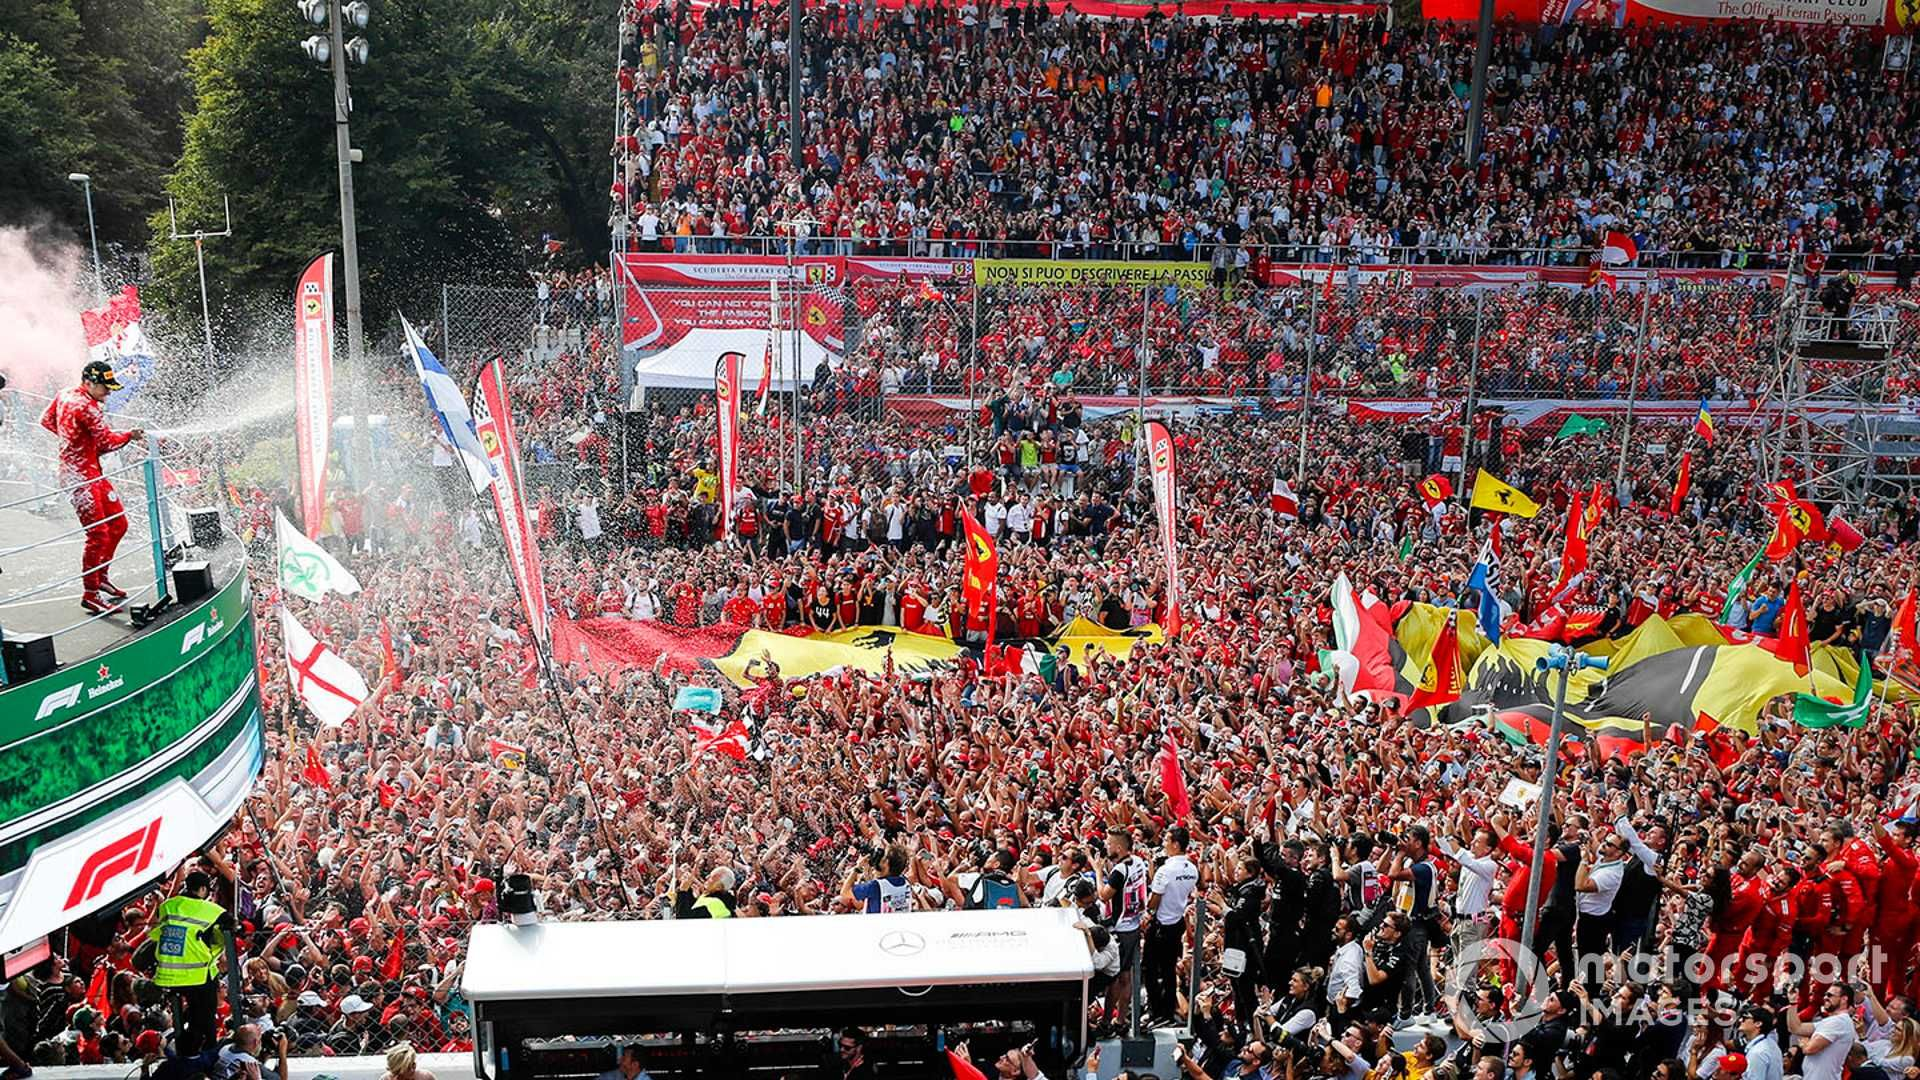
\includegraphics{leclerc_monza.jpg}
\end{figure}

    Le dataset ne nous fournit pas la puissance de la voiture, cette donnée
n'étant pas quantifiable (mis à part peut-être la puissance du moteur).
Nous devons donc essayer nous-même de quantifier ce paramètre.

Dans le paddock, les deux ou trois écuries dominatrices arrivent à
réaliser des tours souvent plus d'une seconde plus rapide que les
écuries de milieu de plateau et les backrunners : on cherche donc un
coefficient \(\mu_x\) permettant de modéliser cette disparité. Nous
choisirons \(\mu_x = \frac{1}{tan(0.1x)^{0.7}}\), avec \(x\) la position
au championnat constructeurs de l'année précédente.

    \begin{tcolorbox}[breakable, size=fbox, boxrule=1pt, pad at break*=1mm,colback=cellbackground, colframe=cellborder]
\prompt{In}{incolor}{538}{\boxspacing}
\begin{Verbatim}[commandchars=\\\{\}]
\PY{k}{def} \PY{n+nf}{prepareDataset}\PY{p}{(}\PY{n}{raceId}\PY{p}{)}\PY{p}{:}
    \PY{l+s+sd}{\PYZsq{}\PYZsq{}\PYZsq{}}
\PY{l+s+sd}{    Cette fonction renvoie, pour une course, les résultats de cette course agrémentés des coefficients.}
\PY{l+s+sd}{    \PYZsq{}\PYZsq{}\PYZsq{}}
    \PY{n}{result} \PY{o}{=} \PY{n}{results}\PY{p}{[}\PY{n}{results}\PY{p}{[}\PY{l+s+s1}{\PYZsq{}}\PY{l+s+s1}{raceId}\PY{l+s+s1}{\PYZsq{}}\PY{p}{]} \PY{o}{==} \PY{n}{raceId}\PY{p}{]}
    \PY{n}{year} \PY{o}{=} \PY{n}{races}\PY{p}{[}\PY{l+s+s1}{\PYZsq{}}\PY{l+s+s1}{year}\PY{l+s+s1}{\PYZsq{}}\PY{p}{]}\PY{o}{.}\PY{n}{loc}\PY{p}{[}\PY{n}{raceId}\PY{p}{]}
    \PY{n}{current\PYZus{}round} \PY{o}{=} \PY{n}{races}\PY{p}{[}\PY{l+s+s1}{\PYZsq{}}\PY{l+s+s1}{round}\PY{l+s+s1}{\PYZsq{}}\PY{p}{]}\PY{o}{.}\PY{n}{loc}\PY{p}{[}\PY{n}{raceId}\PY{p}{]}
    \PY{n}{result}\PY{p}{[}\PY{l+s+s1}{\PYZsq{}}\PY{l+s+s1}{constructorPower}\PY{l+s+s1}{\PYZsq{}}\PY{p}{]} \PY{o}{=} \PY{n}{result}\PY{p}{[}\PY{l+s+s1}{\PYZsq{}}\PY{l+s+s1}{constructorId}\PY{l+s+s1}{\PYZsq{}}\PY{p}{]}\PY{o}{.}\PY{n}{apply}\PY{p}{(}\PY{k}{lambda} \PY{n}{x}\PY{p}{:} \PY{l+m+mf}{1.0}\PY{o}{/}\PY{n}{np}\PY{o}{.}\PY{n}{power}\PY{p}{(}\PY{n}{np}\PY{o}{.}\PY{n}{tan}\PY{p}{(}\PY{l+m+mf}{0.1}\PY{o}{*}\PY{n}{getWCCResult}\PY{p}{(}\PY{n}{year}\PY{o}{\PYZhy{}}\PY{l+m+mi}{1}\PY{p}{,}\PY{n}{x}\PY{p}{)}\PY{p}{)}\PY{p}{,}\PY{l+m+mf}{0.7}\PY{p}{)}\PY{p}{)}
    \PY{n}{result}\PY{p}{[}\PY{l+s+s1}{\PYZsq{}}\PY{l+s+s1}{constructorForm}\PY{l+s+s1}{\PYZsq{}}\PY{p}{]} \PY{o}{=} \PY{n}{result}\PY{p}{[}\PY{l+s+s1}{\PYZsq{}}\PY{l+s+s1}{constructorId}\PY{l+s+s1}{\PYZsq{}}\PY{p}{]}\PY{o}{.}\PY{n}{apply}\PY{p}{(}\PY{k}{lambda} \PY{n}{x}\PY{p}{:} \PY{l+m+mf}{1.0}\PY{o}{/}\PY{n}{np}\PY{o}{.}\PY{n}{power}\PY{p}{(}\PY{n}{np}\PY{o}{.}\PY{n}{tan}\PY{p}{(}\PY{l+m+mf}{0.1}\PY{o}{*}\PY{n}{getWCCPosition}\PY{p}{(}\PY{n}{year}\PY{p}{,}\PY{n}{current\PYZus{}round}\PY{p}{,}\PY{n}{x}\PY{p}{)}\PY{p}{)}\PY{p}{,}\PY{l+m+mf}{0.7}\PY{p}{)}\PY{p}{)}
    \PY{n}{result} \PY{o}{=} \PY{n}{result}\PY{p}{[}\PY{p}{[}\PY{l+s+s1}{\PYZsq{}}\PY{l+s+s1}{driverId}\PY{l+s+s1}{\PYZsq{}}\PY{p}{,}\PY{l+s+s1}{\PYZsq{}}\PY{l+s+s1}{constructorId}\PY{l+s+s1}{\PYZsq{}}\PY{p}{,}\PY{l+s+s1}{\PYZsq{}}\PY{l+s+s1}{grid}\PY{l+s+s1}{\PYZsq{}}\PY{p}{,}\PY{l+s+s1}{\PYZsq{}}\PY{l+s+s1}{positionOrder}\PY{l+s+s1}{\PYZsq{}}\PY{p}{,}\PY{l+s+s1}{\PYZsq{}}\PY{l+s+s1}{points}\PY{l+s+s1}{\PYZsq{}}\PY{p}{,}\PY{l+s+s1}{\PYZsq{}}\PY{l+s+s1}{statusId}\PY{l+s+s1}{\PYZsq{}}\PY{p}{,}\PY{l+s+s1}{\PYZsq{}}\PY{l+s+s1}{constructorPower}\PY{l+s+s1}{\PYZsq{}}\PY{p}{,}\PY{l+s+s1}{\PYZsq{}}\PY{l+s+s1}{constructorForm}\PY{l+s+s1}{\PYZsq{}}\PY{p}{]}\PY{p}{]}\PY{o}{.}\PY{n}{sort\PYZus{}values}\PY{p}{(}\PY{l+s+s1}{\PYZsq{}}\PY{l+s+s1}{grid}\PY{l+s+s1}{\PYZsq{}}\PY{p}{)}
    \PY{k}{return} \PY{n}{result}
\end{Verbatim}
\end{tcolorbox}

    \begin{tcolorbox}[breakable, size=fbox, boxrule=1pt, pad at break*=1mm,colback=cellbackground, colframe=cellborder]
\prompt{In}{incolor}{570}{\boxspacing}
\begin{Verbatim}[commandchars=\\\{\}]
\PY{n}{my\PYZus{}dataset} \PY{o}{=} \PY{n}{prepareDataset}\PY{p}{(}\PY{l+m+mi}{1}\PY{p}{)}
\PY{k}{print}\PY{p}{(}\PY{n}{races}\PY{o}{.}\PY{n}{shape}\PY{p}{[}\PY{l+m+mi}{0}\PY{p}{]}\PY{p}{)}
\PY{k}{for} \PY{n}{i} \PY{o+ow}{in} \PY{n+nb}{range}\PY{p}{(}\PY{l+m+mi}{2}\PY{p}{,} \PY{n}{races}\PY{o}{.}\PY{n}{shape}\PY{p}{[}\PY{l+m+mi}{0}\PY{p}{]}\PY{p}{)}\PY{p}{:}
    \PY{k}{print}\PY{p}{(}\PY{l+s+s2}{\PYZdq{}}\PY{l+s+s2}{\PYZob{}\PYZcb{}/\PYZob{}\PYZcb{}}\PY{l+s+se}{\PYZbs{}r}\PY{l+s+s2}{\PYZdq{}}\PY{o}{.}\PY{n}{format}\PY{p}{(}\PY{n}{i}\PY{p}{,}\PY{n}{races}\PY{o}{.}\PY{n}{shape}\PY{p}{[}\PY{l+m+mi}{0}\PY{p}{]}\PY{p}{)}\PY{p}{)}\PY{p}{,}
    \PY{n}{my\PYZus{}dataset} \PY{o}{=} \PY{n}{my\PYZus{}dataset}\PY{o}{.}\PY{n}{append}\PY{p}{(}\PY{n}{prepareDataset}\PY{p}{(}\PY{n}{i}\PY{p}{)}\PY{p}{)}
    
\PY{n}{display}\PY{p}{(}\PY{n}{my\PYZus{}dataset}\PY{p}{)}
\end{Verbatim}
\end{tcolorbox}


\begin{tcolorbox}[breakable, size=fbox, boxrule=1pt, pad at break*=1mm,colback=cellbackground, colframe=cellborder]
\prompt{In}{incolor}{571}{\boxspacing}
\begin{Verbatim}[commandchars=\\\{\}]
\PY{n}{my\PYZus{}dataset}\PY{o}{.}\PY{n}{describe}\PY{p}{(}\PY{p}{)}
\PY{n}{my\PYZus{}dataset} \PY{o}{=} \PY{n}{my\PYZus{}dataset}\PY{p}{[}\PY{p}{(}\PY{n}{my\PYZus{}dataset}\PY{p}{[}\PY{l+s+s1}{\PYZsq{}}\PY{l+s+s1}{statusId}\PY{l+s+s1}{\PYZsq{}}\PY{p}{]} \PY{o}{==} \PY{l+m+mi}{1}\PY{p}{)} \PY{o}{|} \PY{p}{(}\PY{n}{my\PYZus{}dataset}\PY{p}{[}\PY{l+s+s1}{\PYZsq{}}\PY{l+s+s1}{statusId}\PY{l+s+s1}{\PYZsq{}}\PY{p}{]} \PY{o}{==} \PY{l+m+mi}{11}\PY{p}{)} \PY{o}{|} \PY{p}{(}\PY{n}{my\PYZus{}dataset}\PY{p}{[}\PY{l+s+s1}{\PYZsq{}}\PY{l+s+s1}{statusId}\PY{l+s+s1}{\PYZsq{}}\PY{p}{]} \PY{o}{==} \PY{l+m+mi}{12}\PY{p}{)}\PY{p}{]}
\PY{n}{my\PYZus{}dataset} \PY{o}{=} \PY{n}{my\PYZus{}dataset}\PY{p}{[}\PY{p}{[}\PY{l+s+s1}{\PYZsq{}}\PY{l+s+s1}{grid}\PY{l+s+s1}{\PYZsq{}}\PY{p}{,}\PY{l+s+s1}{\PYZsq{}}\PY{l+s+s1}{positionOrder}\PY{l+s+s1}{\PYZsq{}}\PY{p}{,}\PY{l+s+s1}{\PYZsq{}}\PY{l+s+s1}{constructorPower}\PY{l+s+s1}{\PYZsq{}}\PY{p}{,}\PY{l+s+s1}{\PYZsq{}}\PY{l+s+s1}{constructorForm}\PY{l+s+s1}{\PYZsq{}}\PY{p}{]}\PY{p}{]}
\end{Verbatim}
\end{tcolorbox}

    \begin{tcolorbox}[breakable, size=fbox, boxrule=1pt, pad at break*=1mm,colback=cellbackground, colframe=cellborder]
\prompt{In}{incolor}{574}{\boxspacing}
\begin{Verbatim}[commandchars=\\\{\}]
\PY{n}{my\PYZus{}dataset} \PY{o}{=} \PY{n}{my\PYZus{}dataset}\PY{o}{.}\PY{n}{reindex}\PY{p}{(}\PY{n}{np}\PY{o}{.}\PY{n}{random}\PY{o}{.}\PY{n}{permutation}\PY{p}{(}\PY{n}{my\PYZus{}dataset}\PY{o}{.}\PY{n}{index}\PY{p}{)}\PY{p}{)}
\PY{n}{display}\PY{p}{(}\PY{n}{my\PYZus{}dataset}\PY{o}{.}\PY{n}{head}\PY{p}{(}\PY{l+m+mi}{40}\PY{p}{)}\PY{p}{)}
\end{Verbatim}
\end{tcolorbox}


    
    \begin{tcolorbox}[breakable, size=fbox, boxrule=1pt, pad at break*=1mm,colback=cellbackground, colframe=cellborder]
\prompt{In}{incolor}{575}{\boxspacing}
\begin{Verbatim}[commandchars=\\\{\}]
\PY{c+c1}{\PYZsh{} my\PYZus{}dataset.plot(x=\PYZsq{}grid\PYZsq{}, y=\PYZsq{}positionOrder\PYZsq{}, style=\PYZsq{}o\PYZsq{})  }
\PY{c+c1}{\PYZsh{} plt.title(\PYZsq{}MinTemp vs MaxTemp\PYZsq{})  }
\PY{c+c1}{\PYZsh{} plt.xlabel(\PYZsq{}Constructor Power\PYZsq{})  }
\PY{c+c1}{\PYZsh{} plt.ylabel(\PYZsq{}Grid position\PYZsq{})  }
\PY{c+c1}{\PYZsh{} plt.show()}

\PY{n}{sns}\PY{o}{.}\PY{n}{jointplot}\PY{p}{(}\PY{n}{my\PYZus{}dataset}\PY{p}{[}\PY{l+s+s1}{\PYZsq{}}\PY{l+s+s1}{grid}\PY{l+s+s1}{\PYZsq{}}\PY{p}{]}\PY{p}{,}\PY{n}{my\PYZus{}dataset}\PY{p}{[}\PY{l+s+s1}{\PYZsq{}}\PY{l+s+s1}{positionOrder}\PY{l+s+s1}{\PYZsq{}}\PY{p}{]}\PY{p}{,}
              \PY{n}{kind}\PY{o}{=}\PY{l+s+s1}{\PYZsq{}}\PY{l+s+s1}{hex}\PY{l+s+s1}{\PYZsq{}}\PY{p}{)}
\PY{n}{plt}\PY{o}{.}\PY{n}{suptitle}\PY{p}{(}\PY{l+s+s2}{\PYZdq{}}\PY{l+s+s2}{Position a l}\PY{l+s+s2}{\PYZsq{}}\PY{l+s+s2}{arrivee en fonction de la position de depart}\PY{l+s+s2}{\PYZdq{}}\PY{p}{)}

\PY{n}{sns}\PY{o}{.}\PY{n}{jointplot}\PY{p}{(}\PY{n}{my\PYZus{}dataset}\PY{p}{[}\PY{l+s+s1}{\PYZsq{}}\PY{l+s+s1}{constructorPower}\PY{l+s+s1}{\PYZsq{}}\PY{p}{]}\PY{p}{,}\PY{n}{my\PYZus{}dataset}\PY{p}{[}\PY{l+s+s1}{\PYZsq{}}\PY{l+s+s1}{positionOrder}\PY{l+s+s1}{\PYZsq{}}\PY{p}{]}\PY{p}{,}
              \PY{n}{kind}\PY{o}{=}\PY{l+s+s1}{\PYZsq{}}\PY{l+s+s1}{hex}\PY{l+s+s1}{\PYZsq{}}\PY{p}{)}
\PY{n}{plt}\PY{o}{.}\PY{n}{suptitle}\PY{p}{(}\PY{l+s+s2}{\PYZdq{}}\PY{l+s+s2}{Position a l}\PY{l+s+s2}{\PYZsq{}}\PY{l+s+s2}{arrivee en fonction de la position au championnat n\PYZhy{}1}\PY{l+s+s2}{\PYZdq{}}\PY{p}{)}

\PY{n}{sns}\PY{o}{.}\PY{n}{jointplot}\PY{p}{(}\PY{n}{my\PYZus{}dataset}\PY{p}{[}\PY{l+s+s1}{\PYZsq{}}\PY{l+s+s1}{constructorForm}\PY{l+s+s1}{\PYZsq{}}\PY{p}{]}\PY{p}{,}\PY{n}{my\PYZus{}dataset}\PY{p}{[}\PY{l+s+s1}{\PYZsq{}}\PY{l+s+s1}{positionOrder}\PY{l+s+s1}{\PYZsq{}}\PY{p}{]}\PY{p}{,}
              \PY{n}{kind}\PY{o}{=}\PY{l+s+s1}{\PYZsq{}}\PY{l+s+s1}{hex}\PY{l+s+s1}{\PYZsq{}}\PY{p}{)}
\PY{n}{plt}\PY{o}{.}\PY{n}{suptitle}\PY{p}{(}\PY{l+s+s2}{\PYZdq{}}\PY{l+s+s2}{Position a l}\PY{l+s+s2}{\PYZsq{}}\PY{l+s+s2}{arrivee en fonction de la position au championnat}\PY{l+s+s2}{\PYZdq{}}\PY{p}{)}
\end{Verbatim}
\end{tcolorbox}

            \begin{tcolorbox}[breakable, size=fbox, boxrule=.5pt, pad at break*=1mm, opacityfill=0]
\prompt{Out}{outcolor}{575}{\boxspacing}
\begin{Verbatim}[commandchars=\\\{\}]
Text(0.5,0.98,"Position a l'arrivee en fonction de la position au championnat")
\end{Verbatim}
\end{tcolorbox}
        
    \begin{center}
    \adjustimage{max size={0.9\linewidth}{0.9\paperheight}}{output_18_1.png}
    \end{center}
    { \hspace*{\fill} \\}
    
    \begin{center}
    \adjustimage{max size={0.9\linewidth}{0.9\paperheight}}{output_18_2.png}
    \end{center}
    { \hspace*{\fill} \\}
    
    \begin{center}
    \adjustimage{max size={0.9\linewidth}{0.9\paperheight}}{output_18_3.png}
    \end{center}
    { \hspace*{\fill} \\}
    
    \begin{tcolorbox}[breakable, size=fbox, boxrule=1pt, pad at break*=1mm,colback=cellbackground, colframe=cellborder]
\prompt{In}{incolor}{576}{\boxspacing}
\begin{Verbatim}[commandchars=\\\{\}]
\PY{n}{my\PYZus{}dataset} \PY{o}{=} \PY{n}{my\PYZus{}dataset}\PY{o}{.}\PY{n}{dropna}\PY{p}{(}\PY{p}{)}

\PY{n}{train\PYZus{}dataset} \PY{o}{=} \PY{n}{my\PYZus{}dataset}\PY{o}{.}\PY{n}{sample}\PY{p}{(}\PY{n}{frac}\PY{o}{=}\PY{l+m+mf}{0.8}\PY{p}{,}\PY{n}{random\PYZus{}state}\PY{o}{=}\PY{l+m+mi}{1}\PY{p}{)}
\PY{n}{test\PYZus{}dataset} \PY{o}{=} \PY{n}{my\PYZus{}dataset}\PY{o}{.}\PY{n}{drop}\PY{p}{(}\PY{n}{train\PYZus{}dataset}\PY{o}{.}\PY{n}{index}\PY{p}{)}

\PY{n}{train\PYZus{}stats} \PY{o}{=} \PY{n}{train\PYZus{}dataset}\PY{o}{.}\PY{n}{describe}\PY{p}{(}\PY{p}{)}
\PY{n}{train\PYZus{}stats}\PY{o}{.}\PY{n}{pop}\PY{p}{(}\PY{l+s+s2}{\PYZdq{}}\PY{l+s+s2}{positionOrder}\PY{l+s+s2}{\PYZdq{}}\PY{p}{)}
\PY{n}{train\PYZus{}stats} \PY{o}{=} \PY{n}{train\PYZus{}stats}\PY{o}{.}\PY{n}{transpose}\PY{p}{(}\PY{p}{)}

\PY{n}{train\PYZus{}labels} \PY{o}{=} \PY{n}{train\PYZus{}dataset}\PY{o}{.}\PY{n}{pop}\PY{p}{(}\PY{l+s+s1}{\PYZsq{}}\PY{l+s+s1}{positionOrder}\PY{l+s+s1}{\PYZsq{}}\PY{p}{)}
\PY{n}{test\PYZus{}labels} \PY{o}{=} \PY{n}{test\PYZus{}dataset}\PY{o}{.}\PY{n}{pop}\PY{p}{(}\PY{l+s+s1}{\PYZsq{}}\PY{l+s+s1}{positionOrder}\PY{l+s+s1}{\PYZsq{}}\PY{p}{)}

\PY{k}{def} \PY{n+nf}{norm}\PY{p}{(}\PY{n}{x}\PY{p}{)}\PY{p}{:}
  \PY{k}{return} \PY{p}{(}\PY{n}{x} \PY{o}{\PYZhy{}} \PY{n}{train\PYZus{}stats}\PY{p}{[}\PY{l+s+s1}{\PYZsq{}}\PY{l+s+s1}{mean}\PY{l+s+s1}{\PYZsq{}}\PY{p}{]}\PY{p}{)} \PY{o}{/} \PY{n}{train\PYZus{}stats}\PY{p}{[}\PY{l+s+s1}{\PYZsq{}}\PY{l+s+s1}{std}\PY{l+s+s1}{\PYZsq{}}\PY{p}{]}
\PY{n}{normed\PYZus{}train\PYZus{}data} \PY{o}{=} \PY{n}{norm}\PY{p}{(}\PY{n}{train\PYZus{}dataset}\PY{p}{)}
\PY{n}{normed\PYZus{}test\PYZus{}data} \PY{o}{=} \PY{n}{norm}\PY{p}{(}\PY{n}{test\PYZus{}dataset}\PY{p}{)}

\PY{n}{display}\PY{p}{(}\PY{n}{normed\PYZus{}test\PYZus{}data}\PY{o}{.}\PY{n}{head}\PY{p}{(}\PY{l+m+mi}{20}\PY{p}{)}\PY{p}{)}
\end{Verbatim}
\end{tcolorbox}


    
    \hypertarget{cruxe9ation-du-moduxe8le-avec-tensorflow}{%
\subsubsection{Création du modèle avec
TensorFlow}\label{cruxe9ation-du-moduxe8le-avec-tensorflow}}

Typiquement, TensorFlow permet d'obtenir une bonne précision sur les
résultats si on sait ce qu'on fait. Nous allons créer et entraîner un
modèle TensorFlow puis comparer ses prédictions avec notre propre
modèle.

    \begin{tcolorbox}[breakable, size=fbox, boxrule=1pt, pad at break*=1mm,colback=cellbackground, colframe=cellborder]
\prompt{In}{incolor}{577}{\boxspacing}
\begin{Verbatim}[commandchars=\\\{\}]
\PY{k}{def} \PY{n+nf}{build\PYZus{}model}\PY{p}{(}\PY{p}{)}\PY{p}{:}
  \PY{n}{model} \PY{o}{=} \PY{n}{keras}\PY{o}{.}\PY{n}{Sequential}\PY{p}{(}\PY{p}{[}
    \PY{n}{keras}\PY{o}{.}\PY{n}{layers}\PY{o}{.}\PY{n}{Dense}\PY{p}{(}\PY{l+m+mi}{64}\PY{p}{,} \PY{n}{activation}\PY{o}{=}\PY{l+s+s1}{\PYZsq{}}\PY{l+s+s1}{relu}\PY{l+s+s1}{\PYZsq{}}\PY{p}{,} \PY{n}{input\PYZus{}shape}\PY{o}{=}\PY{p}{[}\PY{n+nb}{len}\PY{p}{(}\PY{n}{train\PYZus{}dataset}\PY{o}{.}\PY{n}{keys}\PY{p}{(}\PY{p}{)}\PY{p}{)}\PY{p}{]}\PY{p}{)}\PY{p}{,}
    \PY{n}{keras}\PY{o}{.}\PY{n}{layers}\PY{o}{.}\PY{n}{Dense}\PY{p}{(}\PY{l+m+mi}{64}\PY{p}{,} \PY{n}{activation}\PY{o}{=}\PY{l+s+s1}{\PYZsq{}}\PY{l+s+s1}{relu}\PY{l+s+s1}{\PYZsq{}}\PY{p}{)}\PY{p}{,}
    \PY{n}{keras}\PY{o}{.}\PY{n}{layers}\PY{o}{.}\PY{n}{Dense}\PY{p}{(}\PY{l+m+mi}{1}\PY{p}{)}
  \PY{p}{]}\PY{p}{)}

  \PY{n}{optimizer} \PY{o}{=} \PY{n}{tf}\PY{o}{.}\PY{n}{keras}\PY{o}{.}\PY{n}{optimizers}\PY{o}{.}\PY{n}{RMSprop}\PY{p}{(}\PY{l+m+mf}{0.001}\PY{p}{)}

  \PY{n}{model}\PY{o}{.}\PY{n}{compile}\PY{p}{(}\PY{n}{loss}\PY{o}{=}\PY{l+s+s1}{\PYZsq{}}\PY{l+s+s1}{mse}\PY{l+s+s1}{\PYZsq{}}\PY{p}{,}
                \PY{n}{optimizer}\PY{o}{=}\PY{n}{optimizer}\PY{p}{,}
                \PY{n}{metrics}\PY{o}{=}\PY{p}{[}\PY{l+s+s1}{\PYZsq{}}\PY{l+s+s1}{mae}\PY{l+s+s1}{\PYZsq{}}\PY{p}{,} \PY{l+s+s1}{\PYZsq{}}\PY{l+s+s1}{mse}\PY{l+s+s1}{\PYZsq{}}\PY{p}{]}\PY{p}{)}
  \PY{k}{return} \PY{n}{model}
\PY{n}{model} \PY{o}{=} \PY{n}{build\PYZus{}model}\PY{p}{(}\PY{p}{)}
\end{Verbatim}
\end{tcolorbox}

    \begin{tcolorbox}[breakable, size=fbox, boxrule=1pt, pad at break*=1mm,colback=cellbackground, colframe=cellborder]
\prompt{In}{incolor}{578}{\boxspacing}
\begin{Verbatim}[commandchars=\\\{\}]
\PY{n}{EPOCHS} \PY{o}{=} \PY{l+m+mi}{100}

\PY{n}{history} \PY{o}{=} \PY{n}{model}\PY{o}{.}\PY{n}{fit}\PY{p}{(}
  \PY{n}{normed\PYZus{}train\PYZus{}data}\PY{p}{,} \PY{n}{train\PYZus{}labels}\PY{p}{,}
  \PY{n}{epochs}\PY{o}{=}\PY{n}{EPOCHS}\PY{p}{,} \PY{n}{validation\PYZus{}split} \PY{o}{=} \PY{l+m+mf}{0.2}\PY{p}{,} \PY{n}{verbose}\PY{o}{=}\PY{l+m+mi}{1}\PY{p}{)}
\PY{n}{test\PYZus{}predictions} \PY{o}{=} \PY{n}{model}\PY{o}{.}\PY{n}{predict}\PY{p}{(}\PY{n}{normed\PYZus{}test\PYZus{}data}\PY{p}{)}\PY{o}{.}\PY{n}{flatten}\PY{p}{(}\PY{p}{)}
\end{Verbatim}
\end{tcolorbox}


    \begin{tcolorbox}[breakable, size=fbox, boxrule=1pt, pad at break*=1mm,colback=cellbackground, colframe=cellborder]
\prompt{In}{incolor}{579}{\boxspacing}
\begin{Verbatim}[commandchars=\\\{\}]
\PY{n}{sns}\PY{o}{.}\PY{n}{jointplot}\PY{p}{(}\PY{n}{test\PYZus{}labels}\PY{p}{,} \PY{n}{test\PYZus{}predictions}\PY{p}{,} \PY{n}{kind}\PY{o}{=}\PY{l+s+s1}{\PYZsq{}}\PY{l+s+s1}{hex}\PY{l+s+s1}{\PYZsq{}}\PY{p}{)}
\PY{n}{plt}\PY{o}{.}\PY{n}{suptitle}\PY{p}{(}\PY{l+s+s1}{\PYZsq{}}\PY{l+s+s1}{Valeurs predites par TensorFlow contre vraies valeurs}\PY{l+s+s1}{\PYZsq{}}\PY{p}{)}
\end{Verbatim}
\end{tcolorbox}

            \begin{tcolorbox}[breakable, size=fbox, boxrule=.5pt, pad at break*=1mm, opacityfill=0]
\prompt{Out}{outcolor}{579}{\boxspacing}
\begin{Verbatim}[commandchars=\\\{\}]
Text(0.5,0.98,'Valeurs predites par TensorFlow contre vraies valeurs')
\end{Verbatim}
\end{tcolorbox}
        
    \begin{center}
    \adjustimage{max size={0.9\linewidth}{0.9\paperheight}}{output_23_1.png}
    \end{center}
    { \hspace*{\fill} \\}
    
    \begin{tcolorbox}[breakable, size=fbox, boxrule=1pt, pad at break*=1mm,colback=cellbackground, colframe=cellborder]
\prompt{In}{incolor}{580}{\boxspacing}
\begin{Verbatim}[commandchars=\\\{\}]
\PY{n}{TFError} \PY{o}{=} \PY{n}{test\PYZus{}predictions} \PY{o}{\PYZhy{}} \PY{n}{test\PYZus{}labels}
\PY{n}{fig}\PY{p}{,} \PY{n}{ax} \PY{o}{=} \PY{n}{plt}\PY{o}{.}\PY{n}{subplots}\PY{p}{(}\PY{l+m+mi}{1}\PY{p}{,}\PY{l+m+mi}{1}\PY{p}{)}
\PY{n}{plt}\PY{o}{.}\PY{n}{hist}\PY{p}{(}\PY{n}{TFError}\PY{p}{,} \PY{n}{bins} \PY{o}{=} \PY{l+m+mi}{20}\PY{p}{,} \PY{n}{color}\PY{o}{=}\PY{l+s+s1}{\PYZsq{}}\PY{l+s+s1}{gold}\PY{l+s+s1}{\PYZsq{}}\PY{p}{,}\PY{n}{alpha}\PY{o}{=}\PY{l+m+mf}{0.9}\PY{p}{)}
\PY{n}{ax}\PY{o}{.}\PY{n}{set\PYZus{}facecolor}\PY{p}{(}\PY{l+s+s1}{\PYZsq{}}\PY{l+s+s1}{xkcd:dark grey}\PY{l+s+s1}{\PYZsq{}}\PY{p}{)}
\PY{n}{ax}\PY{o}{.}\PY{n}{grid}\PY{p}{(}\PY{n+nb+bp}{False}\PY{p}{)}

\PY{n}{plt}\PY{o}{.}\PY{n}{xlabel}\PY{p}{(}\PY{l+s+s2}{\PYZdq{}}\PY{l+s+s2}{Erreur sur la prediction avec TensorFlow}\PY{l+s+s2}{\PYZdq{}}\PY{p}{)}
\PY{n}{\PYZus{}} \PY{o}{=} \PY{n}{plt}\PY{o}{.}\PY{n}{ylabel}\PY{p}{(}\PY{l+s+s2}{\PYZdq{}}\PY{l+s+s2}{Nombre}\PY{l+s+s2}{\PYZdq{}}\PY{p}{)}
\end{Verbatim}
\end{tcolorbox}

    \begin{center}
    \adjustimage{max size={0.9\linewidth}{0.9\paperheight}}{output_24_0.png}
    \end{center}
    { \hspace*{\fill} \\}
    
    \hypertarget{cruxe9ation-du-moduxe8le-uxe0-la-mano}{%
\subsubsection{Création du modèle à la
mano}\label{cruxe9ation-du-moduxe8le-uxe0-la-mano}}

Ici, nous allons coder à la main une fonction de descente de gradient
dans le but de créer un modèle de régression linéaire pour prédire la
position à l'arrivée d'un pilote. L'objectif est de pouvoir faire
tourner l'algorithme plus rapidement que Lance Stroll.

    \begin{tcolorbox}[breakable, size=fbox, boxrule=1pt, pad at break*=1mm,colback=cellbackground, colframe=cellborder]
\prompt{In}{incolor}{581}{\boxspacing}
\begin{Verbatim}[commandchars=\\\{\}]
\PY{k}{def} \PY{n+nf}{loss}\PY{p}{(}\PY{n}{predicted\PYZus{}labels}\PY{p}{,}\PY{n}{labels}\PY{p}{)}\PY{p}{:}
    \PY{l+s+sd}{\PYZsq{}\PYZsq{}\PYZsq{}}
\PY{l+s+sd}{    Cette fonction de perte renvoie la MSE (Mean Square Error)}
\PY{l+s+sd}{    \PYZsq{}\PYZsq{}\PYZsq{}}
    \PY{n}{m} \PY{o}{=} \PY{n+nb}{len}\PY{p}{(}\PY{n}{labels}\PY{p}{)}
    \PY{n}{mySum} \PY{o}{=} \PY{l+m+mi}{0}
    \PY{k}{for} \PY{n}{i} \PY{o+ow}{in} \PY{n+nb}{range}\PY{p}{(}\PY{l+m+mi}{0}\PY{p}{,}\PY{n+nb}{len}\PY{p}{(}\PY{n}{labels}\PY{p}{)}\PY{o}{\PYZhy{}}\PY{l+m+mi}{1}\PY{p}{)}\PY{p}{:}
        \PY{n}{mySum} \PY{o}{+}\PY{o}{=} \PY{n}{np}\PY{o}{.}\PY{n}{power}\PY{p}{(}\PY{p}{(}\PY{n}{predicted\PYZus{}labels}\PY{p}{[}\PY{n}{i}\PY{p}{]}\PY{o}{\PYZhy{}}\PY{n}{labels}\PY{p}{[}\PY{n}{i}\PY{p}{]}\PY{p}{)}\PY{p}{,}\PY{l+m+mi}{2}\PY{p}{)}
    \PY{n}{mySum} \PY{o}{=} \PY{p}{(}\PY{l+m+mf}{1.0}\PY{o}{/}\PY{n}{m}\PY{p}{)}\PY{o}{*}\PY{n}{mySum}
    \PY{k}{return} \PY{n}{np}\PY{o}{.}\PY{n}{sqrt}\PY{p}{(}\PY{n}{mySum}\PY{p}{)}


\PY{k}{def} \PY{n+nf}{gradient\PYZus{}descent}\PY{p}{(}\PY{n}{data}\PY{p}{,}\PY{n}{weights}\PY{p}{,}\PY{n}{labels}\PY{p}{,}\PY{n}{speed}\PY{o}{=}\PY{l+m+mf}{0.05}\PY{p}{,}\PY{n}{niter}\PY{o}{=}\PY{l+m+mi}{100}\PY{p}{,}\PY{n}{tol}\PY{o}{=}\PY{l+m+mf}{0.00001}\PY{p}{,}\PY{n}{i}\PY{o}{=}\PY{l+m+mi}{0}\PY{p}{)}\PY{p}{:}
    \PY{l+s+sd}{\PYZsq{}\PYZsq{}\PYZsq{}}
\PY{l+s+sd}{    Weights est un vecteur n colonnes, data est une matrice m lignes n colonnes, les prédictions sont un vecteur m colonnes}
\PY{l+s+sd}{    \PYZsq{}\PYZsq{}\PYZsq{}}
    \PY{n}{prediction} \PY{o}{=} \PY{n}{np}\PY{o}{.}\PY{n}{dot}\PY{p}{(}\PY{n}{data}\PY{p}{,}\PY{n}{weights}\PY{p}{)}
    \PY{n}{coeff} \PY{o}{=} \PY{p}{(}\PY{l+m+mf}{1.0}\PY{o}{*}\PY{n}{speed}\PY{p}{)}\PY{o}{/}\PY{n}{data}\PY{o}{.}\PY{n}{shape}\PY{p}{[}\PY{l+m+mi}{0}\PY{p}{]}
    \PY{n}{lossIter} \PY{o}{=} \PY{n}{loss}\PY{p}{(}\PY{n}{prediction}\PY{p}{,}\PY{n}{labels}\PY{p}{)}
    \PY{k}{for} \PY{n}{j} \PY{o+ow}{in} \PY{n+nb}{range}\PY{p}{(}\PY{l+m+mi}{0}\PY{p}{,}\PY{p}{(}\PY{n}{weights}\PY{o}{.}\PY{n}{shape}\PY{p}{[}\PY{l+m+mi}{0}\PY{p}{]}\PY{p}{)}\PY{p}{)}\PY{p}{:}
        \PY{n}{time}\PY{o}{.}\PY{n}{sleep}\PY{p}{(}\PY{l+m+mf}{0.01}\PY{p}{)}
        \PY{n}{myLoss} \PY{o}{=} \PY{l+m+mi}{0}
        \PY{k}{for} \PY{n}{k} \PY{o+ow}{in} \PY{n+nb}{range}\PY{p}{(}\PY{l+m+mi}{0}\PY{p}{,}\PY{n}{data}\PY{o}{.}\PY{n}{shape}\PY{p}{[}\PY{l+m+mi}{0}\PY{p}{]}\PY{p}{)}\PY{p}{:}
            \PY{n}{myLoss} \PY{o}{+}\PY{o}{=} \PY{p}{(}\PY{n}{prediction}\PY{p}{[}\PY{n}{k}\PY{p}{]}\PY{o}{\PYZhy{}}\PY{n}{labels}\PY{p}{[}\PY{n}{k}\PY{p}{]}\PY{p}{)}\PY{o}{*}\PY{n}{data}\PY{p}{[}\PY{n}{k}\PY{p}{]}\PY{p}{[}\PY{n}{j}\PY{p}{]}
        \PY{k}{print}\PY{p}{(}\PY{l+s+s1}{\PYZsq{}}\PY{l+s+s1}{Itération \PYZob{}\PYZcb{}, weights[0] = \PYZob{}\PYZcb{}, weights[1] = \PYZob{}\PYZcb{}, le cout est de \PYZob{}\PYZcb{}}\PY{l+s+se}{\PYZbs{}r}\PY{l+s+s1}{\PYZsq{}}\PY{o}{.}\PY{n}{format}\PY{p}{(}\PY{n}{i}\PY{p}{,}\PY{n}{weights}\PY{p}{[}\PY{l+m+mi}{0}\PY{p}{]}\PY{p}{,}\PY{n}{weights}\PY{p}{[}\PY{l+m+mi}{1}\PY{p}{]}\PY{p}{,}\PY{n}{myLoss}\PY{p}{)}\PY{p}{)}\PY{p}{,}
        \PY{n}{weights}\PY{p}{[}\PY{n}{j}\PY{p}{]} \PY{o}{=} \PY{p}{(}\PY{n}{weights}\PY{p}{[}\PY{n}{j}\PY{p}{]}\PY{o}{\PYZhy{}}\PY{p}{(}\PY{l+m+mf}{1.0}\PY{o}{*}\PY{n}{coeff}\PY{o}{*}\PY{n}{myLoss}\PY{p}{)}\PY{p}{)}
    \PY{k}{if} \PY{n}{lossIter} \PY{o}{\PYZlt{}} \PY{n}{tol} \PY{o+ow}{or} \PY{n}{i} \PY{o}{\PYZgt{}}\PY{o}{=} \PY{n}{niter}\PY{p}{:}
        \PY{k}{return} \PY{n}{weights}
    \PY{n}{hist}\PY{o}{.}\PY{n}{append}\PY{p}{(}\PY{n}{lossIter}\PY{p}{)}
    \PY{k}{return} \PY{n}{gradient\PYZus{}descent}\PY{p}{(}\PY{n}{data}\PY{p}{,}\PY{n}{weights}\PY{p}{,}\PY{n}{labels}\PY{p}{,}\PY{n}{speed}\PY{p}{,}\PY{n}{niter}\PY{p}{,}\PY{n}{tol}\PY{p}{,}\PY{n}{i}\PY{o}{+}\PY{l+m+mi}{1}\PY{p}{)}

\PY{k}{def} \PY{n+nf}{predict}\PY{p}{(}\PY{n}{data}\PY{p}{,}\PY{n}{weights}\PY{p}{)}\PY{p}{:}
    \PY{k}{return} \PY{n}{np}\PY{o}{.}\PY{n}{dot}\PY{p}{(}\PY{n}{data}\PY{p}{,}\PY{n}{weights}\PY{p}{)}

\PY{n}{hist} \PY{o}{=} \PY{p}{[}\PY{p}{]}
\PY{n}{train} \PY{o}{=} \PY{n}{train\PYZus{}dataset}\PY{o}{.}\PY{n}{to\PYZus{}numpy}\PY{p}{(}\PY{p}{)}
\PY{n}{lab} \PY{o}{=} \PY{n}{train\PYZus{}labels}\PY{o}{.}\PY{n}{to\PYZus{}numpy}\PY{p}{(}\PY{p}{)}
\PY{n}{test} \PY{o}{=} \PY{n}{test\PYZus{}dataset}\PY{o}{.}\PY{n}{to\PYZus{}numpy}\PY{p}{(}\PY{p}{)}
\PY{n}{test\PYZus{}lab} \PY{o}{=} \PY{n}{test\PYZus{}labels}\PY{o}{.}\PY{n}{to\PYZus{}numpy}\PY{p}{(}\PY{p}{)}
\PY{k}{print}\PY{p}{(}\PY{n}{train}\PY{o}{.}\PY{n}{shape}\PY{p}{[}\PY{l+m+mi}{1}\PY{p}{]}\PY{p}{)}
\PY{n}{my\PYZus{}weights} \PY{o}{=} \PY{n}{gradient\PYZus{}descent}\PY{p}{(}\PY{n}{train}\PY{p}{,}\PY{n}{np}\PY{o}{.}\PY{n}{random}\PY{o}{.}\PY{n}{rand}\PY{p}{(}\PY{n}{train}\PY{o}{.}\PY{n}{shape}\PY{p}{[}\PY{l+m+mi}{1}\PY{p}{]}\PY{p}{)}\PY{p}{,}\PY{n}{lab}\PY{p}{,}\PY{n}{speed}\PY{o}{=}\PY{l+m+mf}{0.005}\PY{p}{,} \PY{n}{niter}\PY{o}{=}\PY{l+m+mi}{150}\PY{p}{)}
\PY{n}{my\PYZus{}test} \PY{o}{=} \PY{n}{predict}\PY{p}{(}\PY{n}{test}\PY{p}{,}\PY{n}{my\PYZus{}weights}\PY{p}{)}
\end{Verbatim}
\end{tcolorbox}

    \begin{tcolorbox}[breakable, size=fbox, boxrule=1pt, pad at break*=1mm,colback=cellbackground, colframe=cellborder]
\prompt{In}{incolor}{582}{\boxspacing}
\begin{Verbatim}[commandchars=\\\{\}]
\PY{n}{fig} \PY{o}{=} \PY{n}{plt}\PY{o}{.}\PY{n}{figure}\PY{p}{(}\PY{n}{figsize}\PY{o}{=}\PY{p}{(}\PY{l+m+mi}{8}\PY{p}{,}\PY{l+m+mi}{6}\PY{p}{)}\PY{p}{)}
\PY{n}{ax3} \PY{o}{=} \PY{n}{fig}\PY{o}{.}\PY{n}{add\PYZus{}subplot}\PY{p}{(}\PY{l+m+mi}{111}\PY{p}{)}
\PY{n}{l1}\PY{p}{,} \PY{o}{=} \PY{n}{ax3}\PY{o}{.}\PY{n}{plot}\PY{p}{(}\PY{n}{np}\PY{o}{.}\PY{n}{arange}\PY{p}{(}\PY{n+nb}{len}\PY{p}{(}\PY{n}{hist}\PY{p}{)}\PY{p}{)}\PY{p}{,} \PY{n}{hist}\PY{p}{,} \PY{l+s+s1}{\PYZsq{}}\PY{l+s+s1}{red}\PY{l+s+s1}{\PYZsq{}}\PY{p}{)}
\PY{n}{plt}\PY{o}{.}\PY{n}{suptitle}\PY{p}{(}\PY{l+s+s1}{\PYZsq{}}\PY{l+s+s1}{Evolution de la RMSE en fonction des iterations}\PY{l+s+s1}{\PYZsq{}}\PY{p}{)}
\PY{c+c1}{\PYZsh{} plt.yscale(\PYZsq{}log\PYZsq{})}
\end{Verbatim}
\end{tcolorbox}

            \begin{tcolorbox}[breakable, size=fbox, boxrule=.5pt, pad at break*=1mm, opacityfill=0]
\prompt{Out}{outcolor}{582}{\boxspacing}
\begin{Verbatim}[commandchars=\\\{\}]
Text(0.5,0.98,'Evolution de la RMSE en fonction des iterations')
\end{Verbatim}
\end{tcolorbox}
        
    \begin{center}
    \adjustimage{max size={0.9\linewidth}{0.9\paperheight}}{output_27_1.png}
    \end{center}
    { \hspace*{\fill} \\}
    
    \begin{tcolorbox}[breakable, size=fbox, boxrule=1pt, pad at break*=1mm,colback=cellbackground, colframe=cellborder]
\prompt{In}{incolor}{583}{\boxspacing}
\begin{Verbatim}[commandchars=\\\{\}]
\PY{n}{myplot} \PY{o}{=} \PY{n}{sns}\PY{o}{.}\PY{n}{jointplot}\PY{p}{(}\PY{n}{my\PYZus{}test}\PY{p}{,} \PY{n}{test\PYZus{}lab}\PY{p}{,}\PY{n}{kind}\PY{o}{=}\PY{l+s+s1}{\PYZsq{}}\PY{l+s+s1}{hex}\PY{l+s+s1}{\PYZsq{}}\PY{p}{)}
\PY{n}{plt}\PY{o}{.}\PY{n}{suptitle}\PY{p}{(}\PY{l+s+s2}{\PYZdq{}}\PY{l+s+s2}{Valeurs predites contre vraies valeurs}\PY{l+s+s2}{\PYZdq{}}\PY{p}{)}
\end{Verbatim}
\end{tcolorbox}

            \begin{tcolorbox}[breakable, size=fbox, boxrule=.5pt, pad at break*=1mm, opacityfill=0]
\prompt{Out}{outcolor}{583}{\boxspacing}
\begin{Verbatim}[commandchars=\\\{\}]
Text(0.5,0.98,'Valeurs predites contre vraies valeurs')
\end{Verbatim}
\end{tcolorbox}
        
    \begin{center}
    \adjustimage{max size={0.9\linewidth}{0.9\paperheight}}{output_28_1.png}
    \end{center}
    { \hspace*{\fill} \\}
    
    \begin{tcolorbox}[breakable, size=fbox, boxrule=1pt, pad at break*=1mm,colback=cellbackground, colframe=cellborder]
\prompt{In}{incolor}{584}{\boxspacing}
\begin{Verbatim}[commandchars=\\\{\}]
\PY{n}{error} \PY{o}{=} \PY{n}{my\PYZus{}test} \PY{o}{\PYZhy{}} \PY{n}{test\PYZus{}lab}
\PY{n}{fig}\PY{p}{,} \PY{n}{ax} \PY{o}{=} \PY{n}{plt}\PY{o}{.}\PY{n}{subplots}\PY{p}{(}\PY{l+m+mi}{1}\PY{p}{,}\PY{l+m+mi}{1}\PY{p}{)}
\PY{n}{plt}\PY{o}{.}\PY{n}{hist}\PY{p}{(}\PY{n}{error}\PY{p}{,} \PY{n}{bins} \PY{o}{=} \PY{l+m+mi}{20}\PY{p}{,} \PY{n}{color}\PY{o}{=}\PY{l+s+s1}{\PYZsq{}}\PY{l+s+s1}{gold}\PY{l+s+s1}{\PYZsq{}}\PY{p}{,}\PY{n}{alpha}\PY{o}{=}\PY{l+m+mf}{0.9}\PY{p}{)}
\PY{n}{ax}\PY{o}{.}\PY{n}{set\PYZus{}facecolor}\PY{p}{(}\PY{l+s+s1}{\PYZsq{}}\PY{l+s+s1}{xkcd:dark grey}\PY{l+s+s1}{\PYZsq{}}\PY{p}{)}
\PY{n}{ax}\PY{o}{.}\PY{n}{grid}\PY{p}{(}\PY{n+nb+bp}{False}\PY{p}{)}
\PY{n}{plt}\PY{o}{.}\PY{n}{xlabel}\PY{p}{(}\PY{l+s+s2}{\PYZdq{}}\PY{l+s+s2}{Erreur sur la prediction}\PY{l+s+s2}{\PYZdq{}}\PY{p}{)}
\PY{n}{\PYZus{}} \PY{o}{=} \PY{n}{plt}\PY{o}{.}\PY{n}{ylabel}\PY{p}{(}\PY{l+s+s2}{\PYZdq{}}\PY{l+s+s2}{Nombre}\PY{l+s+s2}{\PYZdq{}}\PY{p}{)}
\end{Verbatim}
\end{tcolorbox}

    \begin{center}
    \adjustimage{max size={0.9\linewidth}{0.9\paperheight}}{output_29_0.png}
    \end{center}
    { \hspace*{\fill} \\}
    
    On peut remarquer que l'algorithme de descente de gradient ne présente
pas d'overfitting et prédit plutôt bien la position d'arrivée du pilote,
même si l'algorithme de TensorFlow est légèrement plus performant.

    \begin{tcolorbox}[breakable, size=fbox, boxrule=1pt, pad at break*=1mm,colback=cellbackground, colframe=cellborder]
\prompt{In}{incolor}{585}{\boxspacing}
\begin{Verbatim}[commandchars=\\\{\}]
\PY{n}{fig} \PY{o}{=} \PY{n}{plt}\PY{o}{.}\PY{n}{figure}\PY{p}{(}\PY{n}{figsize}\PY{o}{=}\PY{p}{(}\PY{l+m+mi}{14}\PY{p}{,}\PY{l+m+mi}{5}\PY{p}{)}\PY{p}{,}\PY{n}{dpi}\PY{o}{=}\PY{l+m+mi}{300}\PY{p}{)}
\PY{n}{ax2} \PY{o}{=} \PY{n}{fig}\PY{o}{.}\PY{n}{add\PYZus{}subplot}\PY{p}{(}\PY{l+m+mi}{121}\PY{p}{)}
\PY{n}{ax2}\PY{o}{.}\PY{n}{hist}\PY{p}{(}\PY{n}{error}\PY{p}{,} \PY{n}{bins} \PY{o}{=} \PY{l+m+mi}{20}\PY{p}{,} \PY{n}{color}\PY{o}{=}\PY{l+s+s1}{\PYZsq{}}\PY{l+s+s1}{blue}\PY{l+s+s1}{\PYZsq{}}\PY{p}{,}\PY{n}{alpha}\PY{o}{=}\PY{l+m+mf}{0.5}\PY{p}{)}
\PY{n}{ax2}\PY{o}{.}\PY{n}{set\PYZus{}ylabel}\PY{p}{(}\PY{l+s+s1}{\PYZsq{}}\PY{l+s+s1}{Nombre de predictions}\PY{l+s+s1}{\PYZsq{}}\PY{p}{)}
\PY{n}{ax2}\PY{o}{.}\PY{n}{set\PYZus{}xlabel}\PY{p}{(}\PY{l+s+s1}{\PYZsq{}}\PY{l+s+s1}{Erreur (en nombre de positions)}\PY{l+s+s1}{\PYZsq{}}\PY{p}{)}
\PY{n}{ax2}\PY{o}{.}\PY{n}{set\PYZus{}facecolor}\PY{p}{(}\PY{l+s+s1}{\PYZsq{}}\PY{l+s+s1}{xkcd:white}\PY{l+s+s1}{\PYZsq{}}\PY{p}{)}
\PY{n}{plt}\PY{o}{.}\PY{n}{xlim}\PY{p}{(}\PY{o}{\PYZhy{}}\PY{l+m+mi}{10}\PY{p}{,}\PY{l+m+mi}{10}\PY{p}{)}
\PY{n}{ax2}\PY{o}{.}\PY{n}{legend}\PY{p}{(}\PY{p}{)}
\PY{n}{ax2}\PY{o}{.}\PY{n}{grid}\PY{p}{(}\PY{n+nb+bp}{False}\PY{p}{)}
\PY{n}{ax2}\PY{o}{.}\PY{n}{title}\PY{o}{.}\PY{n}{set\PYZus{}text}\PY{p}{(}\PY{l+s+s1}{\PYZsq{}}\PY{l+s+s1}{Descente de gradient}\PY{l+s+s1}{\PYZsq{}}\PY{p}{)}
     
\PY{n}{ax1} \PY{o}{=} \PY{n}{fig}\PY{o}{.}\PY{n}{add\PYZus{}subplot}\PY{p}{(}\PY{l+m+mi}{122}\PY{p}{)}
\PY{n}{ax1}\PY{o}{.}\PY{n}{hist}\PY{p}{(}\PY{n}{TFError}\PY{p}{,} \PY{n}{bins} \PY{o}{=} \PY{l+m+mi}{20}\PY{p}{,} \PY{n}{color}\PY{o}{=}\PY{l+s+s1}{\PYZsq{}}\PY{l+s+s1}{red}\PY{l+s+s1}{\PYZsq{}}\PY{p}{,}\PY{n}{alpha}\PY{o}{=}\PY{l+m+mf}{0.5}\PY{p}{)}
\PY{n}{ax1}\PY{o}{.}\PY{n}{title}\PY{o}{.}\PY{n}{set\PYZus{}text}\PY{p}{(}\PY{l+s+s1}{\PYZsq{}}\PY{l+s+s1}{TensorFlow}\PY{l+s+s1}{\PYZsq{}}\PY{p}{)}
\PY{n}{ax1}\PY{o}{.}\PY{n}{set\PYZus{}facecolor}\PY{p}{(}\PY{l+s+s1}{\PYZsq{}}\PY{l+s+s1}{xkcd:white}\PY{l+s+s1}{\PYZsq{}}\PY{p}{)}
\PY{n}{plt}\PY{o}{.}\PY{n}{xlim}\PY{p}{(}\PY{o}{\PYZhy{}}\PY{l+m+mi}{10}\PY{p}{,}\PY{l+m+mi}{10}\PY{p}{)}
\PY{n}{ax1}\PY{o}{.}\PY{n}{set\PYZus{}xlabel}\PY{p}{(}\PY{l+s+s1}{\PYZsq{}}\PY{l+s+s1}{Erreur (en nombre de positions)}\PY{l+s+s1}{\PYZsq{}}\PY{p}{)}
\PY{n}{ax1}\PY{o}{.}\PY{n}{grid}\PY{p}{(}\PY{n+nb+bp}{False}\PY{p}{)}
\PY{n}{plt}\PY{o}{.}\PY{n}{tight\PYZus{}layout}\PY{p}{(}\PY{p}{)}
\end{Verbatim}
\end{tcolorbox}

    \begin{Verbatim}[commandchars=\\\{\}]
WARNING:matplotlib.legend:No handles with labels found to put in legend.
    \end{Verbatim}

    \begin{center}
    \adjustimage{max size={0.9\linewidth}{0.9\paperheight}}{output_31_1.png}
    \end{center}
    { \hspace*{\fill} \\}
    
    \hypertarget{remplissage-du-dataset-des-pit-stops}{%
\subsection{Remplissage du dataset des
pit-stops}\label{remplissage-du-dataset-des-pit-stops}}

Le dataset que nous utilisons est incomplet : en effet, il ne propose
les informations de pit-stop qu'à partir de la 841e course, alors que
les données des temps au tour sont disponibles pour beaucoup plus de
courses. Nous souhaitons remplir ce dataset.

On remarque qu'un pit-stop est symbolisé sur le graphique des temps au
tour par un pic brusque entre deux tours rapides. Il est donc possible
d'utiliser un algorithme d'apprentissage supervisé pour trouver les
pit-stops à chaque course.

\begin{figure}
\centering
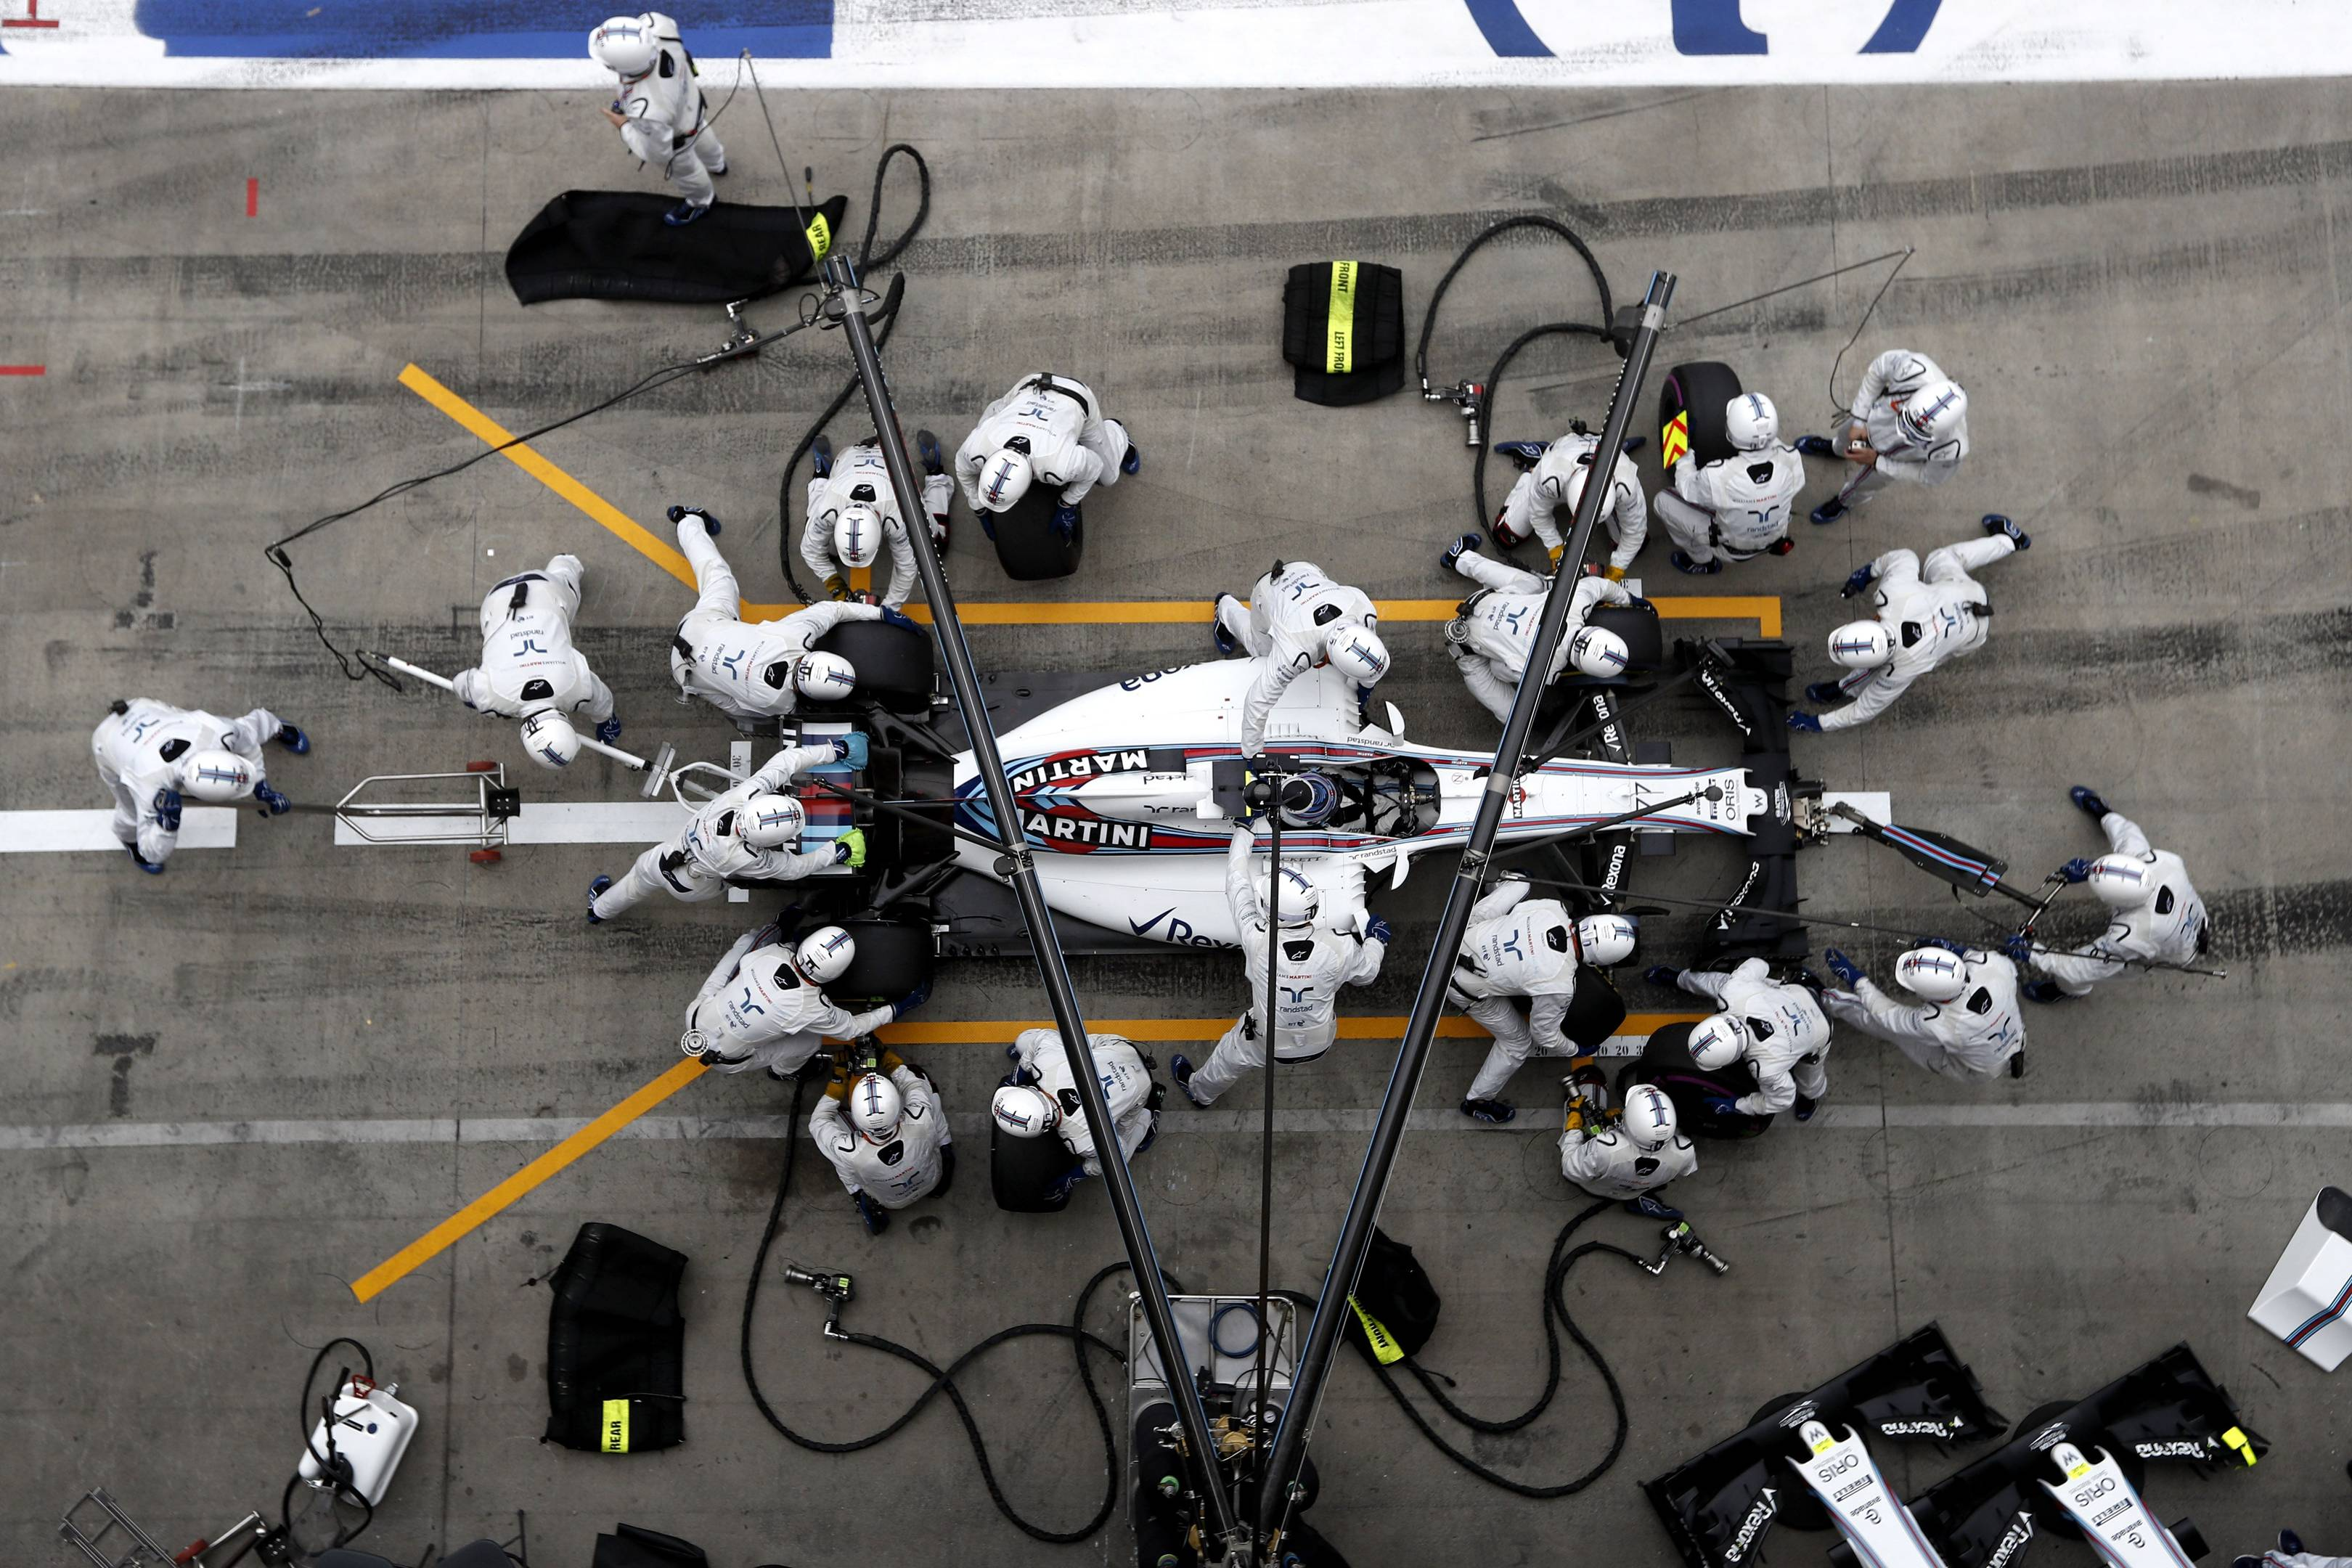
\includegraphics{williams.jpg}
\caption{herothisaustria.jpg}
\end{figure}

    \begin{tcolorbox}[breakable, size=fbox, boxrule=1pt, pad at break*=1mm,colback=cellbackground, colframe=cellborder]
\prompt{In}{incolor}{196}{\boxspacing}
\begin{Verbatim}[commandchars=\\\{\}]
\PY{n}{racesWithPitInformation} \PY{o}{=} \PY{n}{races}
\PY{n}{racesWithoutPitInformation} \PY{o}{=} \PY{n}{races}\PY{o}{.}\PY{n}{iloc}\PY{p}{[}\PY{l+m+mi}{0}\PY{p}{:}\PY{l+m+mi}{0}\PY{p}{]}
\PY{n}{j}\PY{o}{=}\PY{l+m+mi}{0}
\PY{c+c1}{\PYZsh{} for index, row in races.iterrows():}
\PY{c+c1}{\PYZsh{}     if pitStops[pitStops[\PYZsq{}raceId\PYZsq{}] == index].empty:}
\PY{c+c1}{\PYZsh{}         racesWithPitInformation = racesWithPitInformation.drop(index)}
\PY{c+c1}{\PYZsh{}         racesWithoutPitInformation = racesWithoutPitInformation.append(row)}
\end{Verbatim}
\end{tcolorbox}

    Préparation des sets : on va avoir un training set d'environ beaucoup
d'exemples. On peut essayer d'appliquer la technique de cross-validation
pour entraîner le modèle. Quelles sont les features ?

driverId

circuitId

lap

milliseconds

Le label est un vecteur y de taille \(m = nbLaps\). Si le pilote a
réalisé un pit-stop aux tours 4 et 8, on aura
\(y=[0,0,0,1,0,0,0,1,0,...,0]\)

    \begin{tcolorbox}[breakable, size=fbox, boxrule=1pt, pad at break*=1mm,colback=cellbackground, colframe=cellborder]
\prompt{In}{incolor}{258}{\boxspacing}
\begin{Verbatim}[commandchars=\\\{\}]
\PY{c+c1}{\PYZsh{} display(racesWithPitInformation.head())}
\PY{c+c1}{\PYZsh{} display(lapTimes.head())}

\PY{n}{datasetPit} \PY{o}{=} \PY{n}{lapTimes}\PY{o}{.}\PY{n}{merge}\PY{p}{(}\PY{n}{racesWithPitInformation}\PY{p}{,} \PY{n}{on}\PY{o}{=}\PY{l+s+s1}{\PYZsq{}}\PY{l+s+s1}{raceId}\PY{l+s+s1}{\PYZsq{}}\PY{p}{)}
\PY{n}{datasetPit} \PY{o}{=} \PY{n}{datasetPit}\PY{p}{[}\PY{p}{[}\PY{l+s+s1}{\PYZsq{}}\PY{l+s+s1}{raceId}\PY{l+s+s1}{\PYZsq{}}\PY{p}{,}\PY{l+s+s1}{\PYZsq{}}\PY{l+s+s1}{driverId}\PY{l+s+s1}{\PYZsq{}}\PY{p}{,}\PY{l+s+s1}{\PYZsq{}}\PY{l+s+s1}{lap}\PY{l+s+s1}{\PYZsq{}}\PY{p}{,}\PY{l+s+s1}{\PYZsq{}}\PY{l+s+s1}{milliseconds}\PY{l+s+s1}{\PYZsq{}}\PY{p}{,}\PY{l+s+s1}{\PYZsq{}}\PY{l+s+s1}{circuitId}\PY{l+s+s1}{\PYZsq{}}\PY{p}{]}\PY{p}{]}
\PY{n}{datasetPit} \PY{o}{=} \PY{n}{datasetPit}\PY{p}{[}\PY{n}{datasetPit}\PY{p}{[}\PY{l+s+s1}{\PYZsq{}}\PY{l+s+s1}{lap}\PY{l+s+s1}{\PYZsq{}}\PY{p}{]} \PY{o}{\PYZgt{}} \PY{l+m+mi}{5}\PY{p}{]}
\PY{c+c1}{\PYZsh{} for index,row in datasetPit.iterrows():}
\PY{c+c1}{\PYZsh{}     if not pitStops[(pitStops[\PYZsq{}driverId\PYZsq{}] == row[\PYZsq{}driverId\PYZsq{}]) \PYZam{} (pitStops[\PYZsq{}raceId\PYZsq{}] == row[\PYZsq{}raceId\PYZsq{}]) \PYZam{} (pitStops[\PYZsq{}lap\PYZsq{}] == row[\PYZsq{}lap\PYZsq{}])].empty:}
\PY{c+c1}{\PYZsh{}         print(index)}
\PY{c+c1}{\PYZsh{}         datasetPit[\PYZsq{}pit\PYZsq{}].iloc[index] = 1}
\PY{n}{display}\PY{p}{(}\PY{n}{datasetPit}\PY{o}{.}\PY{n}{head}\PY{p}{(}\PY{l+m+mi}{10}\PY{p}{)}\PY{p}{)}
\end{Verbatim}
\end{tcolorbox}

    \begin{tcolorbox}[breakable, size=fbox, boxrule=1pt, pad at break*=1mm,colback=cellbackground, colframe=cellborder]
\prompt{In}{incolor}{586}{\boxspacing}
\begin{Verbatim}[commandchars=\\\{\}]
\PY{n}{my\PYZus{}dataset} \PY{o}{=} \PY{n}{pd}\PY{o}{.}\PY{n}{read\PYZus{}csv}\PY{p}{(}\PY{l+s+s1}{\PYZsq{}}\PY{l+s+s1}{dataset\PYZus{}pit.csv}\PY{l+s+s1}{\PYZsq{}}\PY{p}{,} \PY{n}{index\PYZus{}col}\PY{o}{=}\PY{l+m+mi}{0}\PY{p}{)}
\PY{n}{my\PYZus{}dataset} \PY{o}{=} \PY{n}{my\PYZus{}dataset}\PY{p}{[}\PY{n}{my\PYZus{}dataset}\PY{p}{[}\PY{l+s+s1}{\PYZsq{}}\PY{l+s+s1}{lap}\PY{l+s+s1}{\PYZsq{}}\PY{p}{]} \PY{o}{\PYZgt{}} \PY{l+m+mi}{5}\PY{p}{]}
\PY{n}{my\PYZus{}dataset}\PY{p}{[}\PY{l+s+s1}{\PYZsq{}}\PY{l+s+s1}{previousLap}\PY{l+s+s1}{\PYZsq{}}\PY{p}{]} \PY{o}{=} \PY{n}{np}\PY{o}{.}\PY{n}{zeros}\PY{p}{(}\PY{n}{my\PYZus{}dataset}\PY{o}{.}\PY{n}{shape}\PY{p}{[}\PY{l+m+mi}{0}\PY{p}{]}\PY{p}{)}
\PY{n}{my\PYZus{}dataset\PYZus{}trans} \PY{o}{=} \PY{n}{my\PYZus{}dataset}\PY{o}{.}\PY{n}{shift}\PY{p}{(}\PY{l+m+mi}{1}\PY{p}{)}
\PY{n}{my\PYZus{}dataset\PYZus{}trans}\PY{o}{.}\PY{n}{iloc}\PY{p}{[}\PY{l+m+mi}{0}\PY{p}{]} \PY{o}{=} \PY{n}{my\PYZus{}dataset}\PY{o}{.}\PY{n}{iloc}\PY{p}{[}\PY{l+m+mi}{0}\PY{p}{]}
\PY{n}{my\PYZus{}dataset}\PY{p}{[}\PY{l+s+s1}{\PYZsq{}}\PY{l+s+s1}{previousLap}\PY{l+s+s1}{\PYZsq{}}\PY{p}{]} \PY{o}{=} \PY{n}{my\PYZus{}dataset\PYZus{}trans}\PY{p}{[}\PY{l+s+s1}{\PYZsq{}}\PY{l+s+s1}{milliseconds}\PY{l+s+s1}{\PYZsq{}}\PY{p}{]}
\PY{n}{my\PYZus{}dataset}\PY{p}{[}\PY{l+s+s1}{\PYZsq{}}\PY{l+s+s1}{previousLapRaceId}\PY{l+s+s1}{\PYZsq{}}\PY{p}{]} \PY{o}{=} \PY{n}{my\PYZus{}dataset\PYZus{}trans}\PY{p}{[}\PY{l+s+s1}{\PYZsq{}}\PY{l+s+s1}{raceId}\PY{l+s+s1}{\PYZsq{}}\PY{p}{]}
\PY{n}{my\PYZus{}dataset}\PY{p}{[}\PY{l+s+s1}{\PYZsq{}}\PY{l+s+s1}{previousLapDriverId}\PY{l+s+s1}{\PYZsq{}}\PY{p}{]} \PY{o}{=} \PY{n}{my\PYZus{}dataset\PYZus{}trans}\PY{p}{[}\PY{l+s+s1}{\PYZsq{}}\PY{l+s+s1}{driverId}\PY{l+s+s1}{\PYZsq{}}\PY{p}{]}
\PY{n}{my\PYZus{}dataset}\PY{p}{[}\PY{l+s+s1}{\PYZsq{}}\PY{l+s+s1}{previousLapPit}\PY{l+s+s1}{\PYZsq{}}\PY{p}{]} \PY{o}{=} \PY{n}{my\PYZus{}dataset\PYZus{}trans}\PY{p}{[}\PY{l+s+s1}{\PYZsq{}}\PY{l+s+s1}{pit}\PY{l+s+s1}{\PYZsq{}}\PY{p}{]}
\PY{n}{my\PYZus{}dataset}\PY{p}{[}\PY{l+s+s1}{\PYZsq{}}\PY{l+s+s1}{previousLapDelta}\PY{l+s+s1}{\PYZsq{}}\PY{p}{]} \PY{o}{=} \PY{n}{np}\PY{o}{.}\PY{n}{where}\PY{p}{(}\PY{p}{(}\PY{n}{my\PYZus{}dataset}\PY{p}{[}\PY{l+s+s1}{\PYZsq{}}\PY{l+s+s1}{raceId}\PY{l+s+s1}{\PYZsq{}}\PY{p}{]} \PY{o}{==} \PY{n}{my\PYZus{}dataset}\PY{p}{[}\PY{l+s+s1}{\PYZsq{}}\PY{l+s+s1}{previousLapRaceId}\PY{l+s+s1}{\PYZsq{}}\PY{p}{]}\PY{p}{)} \PY{o}{\PYZam{}} \PY{p}{(}\PY{n}{my\PYZus{}dataset}\PY{p}{[}\PY{l+s+s1}{\PYZsq{}}\PY{l+s+s1}{driverId}\PY{l+s+s1}{\PYZsq{}}\PY{p}{]} \PY{o}{==} \PY{n}{my\PYZus{}dataset}\PY{p}{[}\PY{l+s+s1}{\PYZsq{}}\PY{l+s+s1}{previousLapDriverId}\PY{l+s+s1}{\PYZsq{}}\PY{p}{]}\PY{p}{)} \PY{o}{\PYZam{}} \PY{n}{my\PYZus{}dataset}\PY{p}{[}\PY{l+s+s1}{\PYZsq{}}\PY{l+s+s1}{previousLapPit}\PY{l+s+s1}{\PYZsq{}}\PY{p}{]} \PY{o}{!=} \PY{l+m+mi}{1}\PY{p}{,} \PY{n}{my\PYZus{}dataset}\PY{p}{[}\PY{l+s+s1}{\PYZsq{}}\PY{l+s+s1}{milliseconds}\PY{l+s+s1}{\PYZsq{}}\PY{p}{]}\PY{o}{/}\PY{n}{my\PYZus{}dataset}\PY{p}{[}\PY{l+s+s1}{\PYZsq{}}\PY{l+s+s1}{previousLap}\PY{l+s+s1}{\PYZsq{}}\PY{p}{]}\PY{p}{,} \PY{l+m+mi}{1}\PY{p}{)}

\PY{n}{my\PYZus{}dataset\PYZus{}fwd} \PY{o}{=} \PY{n}{my\PYZus{}dataset}\PY{o}{.}\PY{n}{shift}\PY{p}{(}\PY{o}{\PYZhy{}}\PY{l+m+mi}{1}\PY{p}{)}
\PY{n}{my\PYZus{}dataset\PYZus{}fwd}\PY{o}{.}\PY{n}{loc}\PY{p}{[}\PY{n}{my\PYZus{}dataset\PYZus{}fwd}\PY{o}{.}\PY{n}{shape}\PY{p}{[}\PY{l+m+mi}{0}\PY{p}{]}\PY{p}{]} \PY{o}{=}  \PY{n}{my\PYZus{}dataset}\PY{o}{.}\PY{n}{loc}\PY{p}{[}\PY{n}{my\PYZus{}dataset}\PY{o}{.}\PY{n}{shape}\PY{p}{[}\PY{l+m+mi}{0}\PY{p}{]}\PY{p}{]}
\PY{n}{my\PYZus{}dataset}\PY{p}{[}\PY{l+s+s1}{\PYZsq{}}\PY{l+s+s1}{nextLap}\PY{l+s+s1}{\PYZsq{}}\PY{p}{]} \PY{o}{=} \PY{n}{my\PYZus{}dataset\PYZus{}fwd}\PY{p}{[}\PY{l+s+s1}{\PYZsq{}}\PY{l+s+s1}{milliseconds}\PY{l+s+s1}{\PYZsq{}}\PY{p}{]}
\PY{n}{my\PYZus{}dataset}\PY{p}{[}\PY{l+s+s1}{\PYZsq{}}\PY{l+s+s1}{nextLapRaceId}\PY{l+s+s1}{\PYZsq{}}\PY{p}{]} \PY{o}{=} \PY{n}{my\PYZus{}dataset\PYZus{}fwd}\PY{p}{[}\PY{l+s+s1}{\PYZsq{}}\PY{l+s+s1}{raceId}\PY{l+s+s1}{\PYZsq{}}\PY{p}{]}
\PY{n}{my\PYZus{}dataset}\PY{p}{[}\PY{l+s+s1}{\PYZsq{}}\PY{l+s+s1}{nextLapDriverId}\PY{l+s+s1}{\PYZsq{}}\PY{p}{]} \PY{o}{=} \PY{n}{my\PYZus{}dataset\PYZus{}fwd}\PY{p}{[}\PY{l+s+s1}{\PYZsq{}}\PY{l+s+s1}{driverId}\PY{l+s+s1}{\PYZsq{}}\PY{p}{]}
\PY{n}{my\PYZus{}dataset}\PY{p}{[}\PY{l+s+s1}{\PYZsq{}}\PY{l+s+s1}{nextLapPit}\PY{l+s+s1}{\PYZsq{}}\PY{p}{]} \PY{o}{=} \PY{n}{my\PYZus{}dataset\PYZus{}fwd}\PY{p}{[}\PY{l+s+s1}{\PYZsq{}}\PY{l+s+s1}{pit}\PY{l+s+s1}{\PYZsq{}}\PY{p}{]}
\PY{n}{my\PYZus{}dataset}\PY{p}{[}\PY{l+s+s1}{\PYZsq{}}\PY{l+s+s1}{nextLapDelta}\PY{l+s+s1}{\PYZsq{}}\PY{p}{]} \PY{o}{=} \PY{n}{np}\PY{o}{.}\PY{n}{where}\PY{p}{(}\PY{p}{(}\PY{n}{my\PYZus{}dataset}\PY{p}{[}\PY{l+s+s1}{\PYZsq{}}\PY{l+s+s1}{raceId}\PY{l+s+s1}{\PYZsq{}}\PY{p}{]} \PY{o}{==} \PY{n}{my\PYZus{}dataset}\PY{p}{[}\PY{l+s+s1}{\PYZsq{}}\PY{l+s+s1}{nextLapRaceId}\PY{l+s+s1}{\PYZsq{}}\PY{p}{]}\PY{p}{)} \PY{o}{\PYZam{}} \PY{p}{(}\PY{n}{my\PYZus{}dataset}\PY{p}{[}\PY{l+s+s1}{\PYZsq{}}\PY{l+s+s1}{driverId}\PY{l+s+s1}{\PYZsq{}}\PY{p}{]} \PY{o}{==} \PY{n}{my\PYZus{}dataset}\PY{p}{[}\PY{l+s+s1}{\PYZsq{}}\PY{l+s+s1}{nextLapDriverId}\PY{l+s+s1}{\PYZsq{}}\PY{p}{]}\PY{p}{)} \PY{o}{\PYZam{}} \PY{n}{my\PYZus{}dataset}\PY{p}{[}\PY{l+s+s1}{\PYZsq{}}\PY{l+s+s1}{nextLapPit}\PY{l+s+s1}{\PYZsq{}}\PY{p}{]} \PY{o}{!=} \PY{l+m+mi}{1}\PY{p}{,} \PY{p}{(}\PY{n}{my\PYZus{}dataset}\PY{p}{[}\PY{l+s+s1}{\PYZsq{}}\PY{l+s+s1}{milliseconds}\PY{l+s+s1}{\PYZsq{}}\PY{p}{]}\PY{o}{/}\PY{n}{my\PYZus{}dataset}\PY{p}{[}\PY{l+s+s1}{\PYZsq{}}\PY{l+s+s1}{nextLap}\PY{l+s+s1}{\PYZsq{}}\PY{p}{]}\PY{p}{)}\PY{p}{,} \PY{l+m+mi}{1}\PY{p}{)}

\PY{n}{my\PYZus{}dataset}\PY{p}{[}\PY{l+s+s1}{\PYZsq{}}\PY{l+s+s1}{lapDelta}\PY{l+s+s1}{\PYZsq{}}\PY{p}{]} \PY{o}{=} \PY{p}{(}\PY{n}{my\PYZus{}dataset}\PY{p}{[}\PY{l+s+s1}{\PYZsq{}}\PY{l+s+s1}{previousLapDelta}\PY{l+s+s1}{\PYZsq{}}\PY{p}{]}\PY{o}{+}\PY{n}{my\PYZus{}dataset}\PY{p}{[}\PY{l+s+s1}{\PYZsq{}}\PY{l+s+s1}{nextLapDelta}\PY{l+s+s1}{\PYZsq{}}\PY{p}{]}\PY{p}{)}\PY{o}{/}\PY{l+m+mi}{2}
\PY{n}{my\PYZus{}dataset}\PY{p}{[}\PY{l+s+s1}{\PYZsq{}}\PY{l+s+s1}{lapDelta}\PY{l+s+s1}{\PYZsq{}}\PY{p}{]} \PY{o}{=} \PY{n}{my\PYZus{}dataset}\PY{p}{[}\PY{l+s+s1}{\PYZsq{}}\PY{l+s+s1}{lapDelta}\PY{l+s+s1}{\PYZsq{}}\PY{p}{]}\PY{o}{.}\PY{n}{apply}\PY{p}{(}\PY{k}{lambda} \PY{n}{x}\PY{p}{:} \PY{l+m+mf}{10.0}\PY{o}{*}\PY{p}{(}\PY{l+m+mi}{1}\PY{o}{\PYZhy{}}\PY{n}{np}\PY{o}{.}\PY{n}{exp}\PY{p}{(}\PY{l+m+mi}{1}\PY{o}{\PYZhy{}}\PY{n}{x}\PY{p}{)}\PY{p}{)}\PY{p}{)}
\PY{c+c1}{\PYZsh{} my\PYZus{}dataset[\PYZsq{}lapDelta\PYZsq{}] = (my\PYZus{}dataset[\PYZsq{}lapDelta\PYZsq{}]\PYZhy{}my\PYZus{}dataset[\PYZsq{}lapDelta\PYZsq{}].mean())/my\PYZus{}dataset[\PYZsq{}lapDelta\PYZsq{}].std()}
\PY{n}{my\PYZus{}dataset}\PY{p}{[}\PY{l+s+s1}{\PYZsq{}}\PY{l+s+s1}{lapDelta}\PY{l+s+s1}{\PYZsq{}}\PY{p}{]} \PY{o}{=} \PY{n}{np}\PY{o}{.}\PY{n}{where}\PY{p}{(}\PY{p}{(}\PY{n}{my\PYZus{}dataset}\PY{p}{[}\PY{l+s+s1}{\PYZsq{}}\PY{l+s+s1}{lapDelta}\PY{l+s+s1}{\PYZsq{}}\PY{p}{]} \PY{o}{\PYZlt{}} \PY{l+m+mf}{0.05}\PY{p}{)} \PY{o}{|} \PY{p}{(}\PY{n}{my\PYZus{}dataset}\PY{p}{[}\PY{l+s+s1}{\PYZsq{}}\PY{l+s+s1}{pit}\PY{l+s+s1}{\PYZsq{}}\PY{p}{]} \PY{o}{==} \PY{l+m+mi}{0}\PY{p}{)}\PY{p}{,}\PY{l+m+mi}{0}\PY{p}{,}\PY{l+m+mi}{10}\PY{o}{*}\PY{n}{my\PYZus{}dataset}\PY{p}{[}\PY{l+s+s1}{\PYZsq{}}\PY{l+s+s1}{lapDelta}\PY{l+s+s1}{\PYZsq{}}\PY{p}{]}\PY{p}{)}
\PY{n}{my\PYZus{}dataset} \PY{o}{=} \PY{n}{my\PYZus{}dataset}\PY{o}{.}\PY{n}{drop}\PY{p}{(}\PY{p}{[}\PY{l+s+s1}{\PYZsq{}}\PY{l+s+s1}{previousLap}\PY{l+s+s1}{\PYZsq{}}\PY{p}{,}\PY{l+s+s1}{\PYZsq{}}\PY{l+s+s1}{previousLapRaceId}\PY{l+s+s1}{\PYZsq{}}\PY{p}{,}\PY{l+s+s1}{\PYZsq{}}\PY{l+s+s1}{previousLapDriverId}\PY{l+s+s1}{\PYZsq{}}\PY{p}{,}\PY{l+s+s1}{\PYZsq{}}\PY{l+s+s1}{nextLap}\PY{l+s+s1}{\PYZsq{}}\PY{p}{,}\PY{l+s+s1}{\PYZsq{}}\PY{l+s+s1}{nextLapRaceId}\PY{l+s+s1}{\PYZsq{}}\PY{p}{,}\PY{l+s+s1}{\PYZsq{}}\PY{l+s+s1}{nextLapDriverId}\PY{l+s+s1}{\PYZsq{}}\PY{p}{]}\PY{p}{,}\PY{n}{axis}\PY{o}{=}\PY{l+m+mi}{1}\PY{p}{)}
\PY{k}{for} \PY{n}{i} \PY{o+ow}{in} \PY{n+nb}{range}\PY{p}{(}\PY{l+m+mi}{1}\PY{p}{,}\PY{l+m+mi}{50}\PY{p}{)}\PY{p}{:}
    \PY{n}{my\PYZus{}dataset} \PY{o}{=} \PY{n}{my\PYZus{}dataset}\PY{o}{.}\PY{n}{drop}\PY{p}{(}\PY{n}{my\PYZus{}dataset}\PY{p}{[}\PY{l+s+s1}{\PYZsq{}}\PY{l+s+s1}{previousLapDelta}\PY{l+s+s1}{\PYZsq{}}\PY{p}{]}\PY{o}{.}\PY{n}{idxmax}\PY{p}{(}\PY{p}{)}\PY{p}{)}
    \PY{n}{my\PYZus{}dataset} \PY{o}{=} \PY{n}{my\PYZus{}dataset}\PY{o}{.}\PY{n}{drop}\PY{p}{(}\PY{n}{my\PYZus{}dataset}\PY{p}{[}\PY{l+s+s1}{\PYZsq{}}\PY{l+s+s1}{nextLapDelta}\PY{l+s+s1}{\PYZsq{}}\PY{p}{]}\PY{o}{.}\PY{n}{idxmax}\PY{p}{(}\PY{p}{)}\PY{p}{)}
\PY{n}{display}\PY{p}{(}\PY{n}{my\PYZus{}dataset}\PY{o}{.}\PY{n}{head}\PY{p}{(}\PY{l+m+mi}{10}\PY{p}{)}\PY{p}{)}
\end{Verbatim}
\end{tcolorbox}

    
    
    On peut transformer le problème en un problème de régression logistique
: A un tour donné, quelle est la probablilité qu'un pilote réalise un
arrêt au stand ?

    On peut remarquer ici que seuls 4\% des labels représentent un arrêt au
stand : les données ne sont pas du tout équitablement réparties !!

    \begin{tcolorbox}[breakable, size=fbox, boxrule=1pt, pad at break*=1mm,colback=cellbackground, colframe=cellborder]
\prompt{In}{incolor}{587}{\boxspacing}
\begin{Verbatim}[commandchars=\\\{\}]
\PY{n}{neg}\PY{p}{,} \PY{n}{pos} \PY{o}{=} \PY{n}{np}\PY{o}{.}\PY{n}{bincount}\PY{p}{(}\PY{n}{my\PYZus{}dataset}\PY{p}{[}\PY{l+s+s1}{\PYZsq{}}\PY{l+s+s1}{pit}\PY{l+s+s1}{\PYZsq{}}\PY{p}{]}\PY{p}{)}
\PY{n}{total} \PY{o}{=} \PY{n}{neg} \PY{o}{+} \PY{n}{pos}
\PY{k}{print}\PY{p}{(}\PY{l+s+s1}{\PYZsq{}}\PY{l+s+s1}{Examples:}\PY{l+s+se}{\PYZbs{}n}\PY{l+s+s1}{    Total: \PYZob{}\PYZcb{}}\PY{l+s+se}{\PYZbs{}n}\PY{l+s+s1}{    Positive: \PYZob{}\PYZcb{} (\PYZob{}:.2f\PYZcb{}}\PY{l+s+si}{\PYZpc{} o}\PY{l+s+s1}{f total)}\PY{l+s+se}{\PYZbs{}n}\PY{l+s+s1}{\PYZsq{}}\PY{o}{.}\PY{n}{format}\PY{p}{(}
    \PY{n}{total}\PY{p}{,} \PY{n}{pos}\PY{p}{,} \PY{l+m+mi}{100} \PY{o}{*} \PY{n}{pos} \PY{o}{/} \PY{n}{total}\PY{p}{)}\PY{p}{)}
\end{Verbatim}
\end{tcolorbox}

    \begin{Verbatim}[commandchars=\\\{\}]
Examples:
    Total: 143335
    Positive: 5756 (4.00\% of total)

    \end{Verbatim}

    On crée les ensembles d'entraînement, de validation et de test.

    \begin{tcolorbox}[breakable, size=fbox, boxrule=1pt, pad at break*=1mm,colback=cellbackground, colframe=cellborder]
\prompt{In}{incolor}{588}{\boxspacing}
\begin{Verbatim}[commandchars=\\\{\}]
\PY{n}{cleaned\PYZus{}df} \PY{o}{=} \PY{n}{my\PYZus{}dataset}\PY{p}{[}\PY{p}{[}\PY{l+s+s1}{\PYZsq{}}\PY{l+s+s1}{lapDelta}\PY{l+s+s1}{\PYZsq{}}\PY{p}{,}\PY{l+s+s1}{\PYZsq{}}\PY{l+s+s1}{pit}\PY{l+s+s1}{\PYZsq{}}\PY{p}{]}\PY{p}{]}
\PY{n}{cleaned\PYZus{}df} \PY{o}{=} \PY{n}{cleaned\PYZus{}df}\PY{o}{.}\PY{n}{dropna}\PY{p}{(}\PY{p}{)}
\PY{c+c1}{\PYZsh{} Use a utility from sklearn to split and shuffle our dataset.}
\PY{n}{train\PYZus{}df}\PY{p}{,} \PY{n}{test\PYZus{}df} \PY{o}{=} \PY{n}{train\PYZus{}test\PYZus{}split}\PY{p}{(}\PY{n}{cleaned\PYZus{}df}\PY{p}{,} \PY{n}{test\PYZus{}size}\PY{o}{=}\PY{l+m+mf}{0.2}\PY{p}{)}
\PY{n}{train\PYZus{}df}\PY{p}{,} \PY{n}{val\PYZus{}df} \PY{o}{=} \PY{n}{train\PYZus{}test\PYZus{}split}\PY{p}{(}\PY{n}{train\PYZus{}df}\PY{p}{,} \PY{n}{test\PYZus{}size}\PY{o}{=}\PY{l+m+mf}{0.2}\PY{p}{)}

\PY{c+c1}{\PYZsh{} Form np arrays of labels and features.}
\PY{n}{train\PYZus{}labels} \PY{o}{=} \PY{n}{np}\PY{o}{.}\PY{n}{array}\PY{p}{(}\PY{n}{train\PYZus{}df}\PY{o}{.}\PY{n}{pop}\PY{p}{(}\PY{l+s+s1}{\PYZsq{}}\PY{l+s+s1}{pit}\PY{l+s+s1}{\PYZsq{}}\PY{p}{)}\PY{p}{)}
\PY{n}{bool\PYZus{}train\PYZus{}labels} \PY{o}{=} \PY{n}{train\PYZus{}labels} \PY{o}{!=} \PY{l+m+mi}{0}
\PY{n}{val\PYZus{}labels} \PY{o}{=} \PY{n}{np}\PY{o}{.}\PY{n}{array}\PY{p}{(}\PY{n}{val\PYZus{}df}\PY{o}{.}\PY{n}{pop}\PY{p}{(}\PY{l+s+s1}{\PYZsq{}}\PY{l+s+s1}{pit}\PY{l+s+s1}{\PYZsq{}}\PY{p}{)}\PY{p}{)}
\PY{n}{test\PYZus{}labels} \PY{o}{=} \PY{n}{np}\PY{o}{.}\PY{n}{array}\PY{p}{(}\PY{n}{test\PYZus{}df}\PY{o}{.}\PY{n}{pop}\PY{p}{(}\PY{l+s+s1}{\PYZsq{}}\PY{l+s+s1}{pit}\PY{l+s+s1}{\PYZsq{}}\PY{p}{)}\PY{p}{)}

\PY{n}{train\PYZus{}features} \PY{o}{=} \PY{n}{np}\PY{o}{.}\PY{n}{array}\PY{p}{(}\PY{n}{train\PYZus{}df}\PY{p}{)}
\PY{n}{val\PYZus{}features} \PY{o}{=} \PY{n}{np}\PY{o}{.}\PY{n}{array}\PY{p}{(}\PY{n}{val\PYZus{}df}\PY{p}{)}
\PY{n}{test\PYZus{}features} \PY{o}{=} \PY{n}{np}\PY{o}{.}\PY{n}{array}\PY{p}{(}\PY{n}{test\PYZus{}df}\PY{p}{)}


\PY{c+c1}{\PYZsh{} print(\PYZsq{}Training labels shape:\PYZsq{}, train\PYZus{}labels.shape)}
\PY{c+c1}{\PYZsh{} print(\PYZsq{}Validation labels shape:\PYZsq{}, val\PYZus{}labels.shape)}
\PY{c+c1}{\PYZsh{} print(\PYZsq{}Test labels shape:\PYZsq{}, test\PYZus{}labels.shape)}

\PY{c+c1}{\PYZsh{} print(\PYZsq{}Training features shape:\PYZsq{}, train\PYZus{}features.shape)}
\PY{c+c1}{\PYZsh{} print(\PYZsq{}Validation features shape:\PYZsq{}, val\PYZus{}features.shape)}
\PY{c+c1}{\PYZsh{} print(\PYZsq{}Test features shape:\PYZsq{}, test\PYZus{}features.shape)}

\PY{n}{pit\PYZus{}y} \PY{o}{=} \PY{n}{cleaned\PYZus{}df}\PY{p}{[}\PY{n}{cleaned\PYZus{}df}\PY{p}{[}\PY{l+s+s1}{\PYZsq{}}\PY{l+s+s1}{pit}\PY{l+s+s1}{\PYZsq{}}\PY{p}{]} \PY{o}{==} \PY{l+m+mi}{1}\PY{p}{]}
\PY{n}{pit\PYZus{}n} \PY{o}{=} \PY{n}{cleaned\PYZus{}df}\PY{p}{[}\PY{n}{cleaned\PYZus{}df}\PY{p}{[}\PY{l+s+s1}{\PYZsq{}}\PY{l+s+s1}{pit}\PY{l+s+s1}{\PYZsq{}}\PY{p}{]} \PY{o}{==} \PY{l+m+mi}{0}\PY{p}{]}
\PY{n}{neg} \PY{o}{=} \PY{n}{pit\PYZus{}n}\PY{p}{[}\PY{l+s+s2}{\PYZdq{}}\PY{l+s+s2}{pit}\PY{l+s+s2}{\PYZdq{}}\PY{p}{]}\PY{o}{.}\PY{n}{count}\PY{p}{(}\PY{p}{)}
\PY{n}{pos} \PY{o}{=} \PY{n}{pit\PYZus{}y}\PY{p}{[}\PY{l+s+s1}{\PYZsq{}}\PY{l+s+s1}{pit}\PY{l+s+s1}{\PYZsq{}}\PY{p}{]}\PY{o}{.}\PY{n}{count}\PY{p}{(}\PY{p}{)}
\PY{n}{total} \PY{o}{=} \PY{n}{neg}\PY{o}{+}\PY{n}{pos}
\PY{n}{display}\PY{p}{(}\PY{n}{pit\PYZus{}y}\PY{o}{.}\PY{n}{describe}\PY{p}{(}\PY{p}{)}\PY{p}{)}
\PY{n}{display}\PY{p}{(}\PY{n}{pit\PYZus{}n}\PY{o}{.}\PY{n}{describe}\PY{p}{(}\PY{p}{)}\PY{p}{)}
\PY{c+c1}{\PYZsh{} Scaling by total/2 helps keep the loss to a similar magnitude.}
\PY{c+c1}{\PYZsh{} The sum of the weights of all examples stays the same.}
\PY{n}{weight\PYZus{}for\PYZus{}0} \PY{o}{=} \PY{p}{(}\PY{l+m+mf}{1.0} \PY{o}{/} \PY{n}{neg}\PY{p}{)}\PY{o}{*}\PY{p}{(}\PY{n}{total}\PY{p}{)}\PY{o}{/}\PY{l+m+mf}{2.0} 
\PY{n}{weight\PYZus{}for\PYZus{}1} \PY{o}{=} \PY{p}{(}\PY{l+m+mf}{1.0} \PY{o}{/} \PY{n}{pos}\PY{p}{)}\PY{o}{*}\PY{p}{(}\PY{n}{total}\PY{p}{)}\PY{o}{/}\PY{l+m+mf}{2.0}

\PY{n}{class\PYZus{}weight} \PY{o}{=} \PY{p}{\PYZob{}}\PY{l+m+mi}{0}\PY{p}{:} \PY{n}{weight\PYZus{}for\PYZus{}0}\PY{p}{,} \PY{l+m+mi}{1}\PY{p}{:} \PY{n}{weight\PYZus{}for\PYZus{}1}\PY{p}{\PYZcb{}}

\PY{k}{print}\PY{p}{(}\PY{l+s+s1}{\PYZsq{}}\PY{l+s+s1}{Weight for class 0: \PYZob{}:.2f\PYZcb{}}\PY{l+s+s1}{\PYZsq{}}\PY{o}{.}\PY{n}{format}\PY{p}{(}\PY{n}{weight\PYZus{}for\PYZus{}0}\PY{p}{)}\PY{p}{)}
\PY{k}{print}\PY{p}{(}\PY{l+s+s1}{\PYZsq{}}\PY{l+s+s1}{Weight for class 1: \PYZob{}:.2f\PYZcb{}}\PY{l+s+s1}{\PYZsq{}}\PY{o}{.}\PY{n}{format}\PY{p}{(}\PY{n}{weight\PYZus{}for\PYZus{}1}\PY{p}{)}\PY{p}{)}
\end{Verbatim}
\end{tcolorbox}


    \begin{tcolorbox}[breakable, size=fbox, boxrule=1pt, pad at break*=1mm,colback=cellbackground, colframe=cellborder]
\prompt{In}{incolor}{589}{\boxspacing}
\begin{Verbatim}[commandchars=\\\{\}]
\PY{k}{def} \PY{n+nf}{sigmoid}\PY{p}{(}\PY{n}{x}\PY{p}{)}\PY{p}{:}
    \PY{k}{return} \PY{l+m+mf}{1.0}\PY{o}{/}\PY{p}{(}\PY{l+m+mi}{1}\PY{o}{+}\PY{n}{np}\PY{o}{.}\PY{n}{exp}\PY{p}{(}\PY{o}{\PYZhy{}}\PY{n}{x}\PY{p}{)}\PY{p}{)}

\PY{k}{def} \PY{n+nf}{cost\PYZus{}function}\PY{p}{(}\PY{n}{features}\PY{p}{,} \PY{n}{labels}\PY{p}{,} \PY{n}{weights}\PY{p}{)}\PY{p}{:}
    \PY{n}{observations} \PY{o}{=} \PY{n+nb}{len}\PY{p}{(}\PY{n}{labels}\PY{p}{)}
    \PY{n}{predictions} \PY{o}{=} \PY{n}{predict\PYZus{}logistic}\PY{p}{(}\PY{n}{features}\PY{p}{,} \PY{n}{weights}\PY{p}{)}
    \PY{c+c1}{\PYZsh{}Take the error when label=1}
    \PY{n}{class1\PYZus{}cost} \PY{o}{=} \PY{o}{\PYZhy{}}\PY{n}{labels}\PY{o}{*}\PY{n}{np}\PY{o}{.}\PY{n}{log}\PY{p}{(}\PY{n}{predictions}\PY{p}{)}
    \PY{c+c1}{\PYZsh{}Take the error when label=0}
    \PY{n}{class2\PYZus{}cost} \PY{o}{=} \PY{p}{(}\PY{l+m+mi}{1}\PY{o}{\PYZhy{}}\PY{n}{labels}\PY{p}{)}\PY{o}{*}\PY{n}{np}\PY{o}{.}\PY{n}{log}\PY{p}{(}\PY{l+m+mi}{1}\PY{o}{\PYZhy{}}\PY{n}{predictions}\PY{p}{)}
    \PY{c+c1}{\PYZsh{}Take the sum of both costs}
    \PY{n}{cost} \PY{o}{=} \PY{n}{class1\PYZus{}cost} \PY{o}{\PYZhy{}} \PY{n}{class2\PYZus{}cost}
    \PY{c+c1}{\PYZsh{}Take the average cost}
    \PY{n}{cost} \PY{o}{=} \PY{n}{cost}\PY{o}{.}\PY{n}{sum}\PY{p}{(}\PY{p}{)} \PY{o}{/} \PY{n}{observations}
    \PY{k}{return} \PY{n}{cost}

\PY{k}{def} \PY{n+nf}{update\PYZus{}weights}\PY{p}{(}\PY{n}{features}\PY{p}{,} \PY{n}{labels}\PY{p}{,} \PY{n}{weights}\PY{p}{,} \PY{n}{speed}\PY{p}{)}\PY{p}{:}
    \PY{n}{N} \PY{o}{=} \PY{n+nb}{len}\PY{p}{(}\PY{n}{features}\PY{p}{)}
    \PY{c+c1}{\PYZsh{}1 \PYZhy{} Get Predictions}
    \PY{n}{predictions} \PY{o}{=} \PY{n}{predict\PYZus{}logistic}\PY{p}{(}\PY{n}{features}\PY{p}{,} \PY{n}{weights}\PY{p}{)}
    \PY{c+c1}{\PYZsh{}2 Transpose features from (200, 3) to (3, 200)}
    \PY{c+c1}{\PYZsh{} So we can multiply w the (200,1)  cost matrix.}
    \PY{c+c1}{\PYZsh{} Returns a (3,1) matrix holding 3 partial derivatives \PYZhy{}\PYZhy{}}
    \PY{c+c1}{\PYZsh{} one for each feature \PYZhy{}\PYZhy{} representing the aggregate}
    \PY{c+c1}{\PYZsh{} slope of the cost function across all observations}
    \PY{n}{gradient} \PY{o}{=} \PY{n}{np}\PY{o}{.}\PY{n}{dot}\PY{p}{(}\PY{n}{np}\PY{o}{.}\PY{n}{transpose}\PY{p}{(}\PY{n}{features}\PY{p}{)}\PY{p}{,}  \PY{p}{(}\PY{n}{predictions} \PY{o}{\PYZhy{}} \PY{n}{labels}\PY{p}{)}\PY{p}{)}
    \PY{c+c1}{\PYZsh{}3 Take the average cost derivative for each feature}
    \PY{n}{gradient} \PY{o}{/}\PY{o}{=} \PY{n}{N}
    \PY{c+c1}{\PYZsh{}4 \PYZhy{} Multiply the gradient by our learning rate}
    \PY{n}{gradient} \PY{o}{*}\PY{o}{=} \PY{n}{speed}
    \PY{c+c1}{\PYZsh{}5 \PYZhy{} Subtract from our weights to minimize cost}
    \PY{n}{weights} \PY{o}{\PYZhy{}}\PY{o}{=} \PY{n}{gradient}
    \PY{k}{return} \PY{n}{weights}

\PY{k}{def} \PY{n+nf}{predict\PYZus{}logistic}\PY{p}{(}\PY{n}{features}\PY{p}{,} \PY{n}{weights}\PY{p}{)}\PY{p}{:}
  \PY{l+s+sd}{\PYZsq{}\PYZsq{}\PYZsq{}}
\PY{l+s+sd}{  Returns 1D array of probabilities}
\PY{l+s+sd}{  that the class label == 1}
\PY{l+s+sd}{  \PYZsq{}\PYZsq{}\PYZsq{}}
  \PY{n}{z} \PY{o}{=} \PY{n}{np}\PY{o}{.}\PY{n}{dot}\PY{p}{(}\PY{n}{features}\PY{p}{,} \PY{n}{weights}\PY{p}{)}
  \PY{k}{return} \PY{n}{sigmoid}\PY{p}{(}\PY{n}{z}\PY{p}{)}

\PY{k}{def} \PY{n+nf}{decision\PYZus{}boundary}\PY{p}{(}\PY{n}{prob}\PY{p}{)}\PY{p}{:}
    \PY{k}{return} \PY{l+m+mi}{1} \PY{k}{if} \PY{n}{prob} \PY{o}{\PYZgt{}}\PY{o}{=} \PY{o}{.}\PY{l+m+mi}{5} \PY{k}{else} \PY{l+m+mi}{0}

\PY{k}{def} \PY{n+nf}{classify}\PY{p}{(}\PY{n}{predictions}\PY{p}{)}\PY{p}{:}
    \PY{n}{decision\PYZus{}boundary} \PY{o}{=} \PY{n}{np}\PY{o}{.}\PY{n}{vectorize}\PY{p}{(}\PY{n}{decision\PYZus{}boundary}\PY{p}{)}
    \PY{k}{return} \PY{n}{decision\PYZus{}boundary}\PY{p}{(}\PY{n}{predictions}\PY{p}{)}\PY{o}{.}\PY{n}{flatten}\PY{p}{(}\PY{p}{)}

\PY{k}{def} \PY{n+nf}{train\PYZus{}log}\PY{p}{(}\PY{n}{features}\PY{p}{,} \PY{n}{labels}\PY{p}{,} \PY{n}{weights}\PY{p}{,} \PY{n}{lr}\PY{p}{,} \PY{n}{iters}\PY{p}{)}\PY{p}{:}
    \PY{n}{cost\PYZus{}history} \PY{o}{=} \PY{p}{[}\PY{p}{]}
    \PY{k}{for} \PY{n}{i} \PY{o+ow}{in} \PY{n+nb}{range}\PY{p}{(}\PY{n}{iters}\PY{p}{)}\PY{p}{:}
        \PY{n}{weights} \PY{o}{=} \PY{n}{update\PYZus{}weights}\PY{p}{(}\PY{n}{features}\PY{p}{,} \PY{n}{labels}\PY{p}{,} \PY{n}{weights}\PY{p}{,} \PY{n}{lr}\PY{p}{)}
        \PY{c+c1}{\PYZsh{}Calculate error for auditing purposes}
        \PY{n}{cost} \PY{o}{=} \PY{n}{cost\PYZus{}function}\PY{p}{(}\PY{n}{features}\PY{p}{,} \PY{n}{labels}\PY{p}{,} \PY{n}{weights}\PY{p}{)}
        \PY{n}{cost\PYZus{}history}\PY{o}{.}\PY{n}{append}\PY{p}{(}\PY{n}{cost}\PY{p}{)}
        \PY{k}{print}\PY{p}{(}\PY{l+s+s1}{\PYZsq{}}\PY{l+s+s1}{Itération \PYZob{}\PYZcb{} : la Loss est égale à \PYZob{}\PYZcb{}}\PY{l+s+se}{\PYZbs{}r}\PY{l+s+s1}{\PYZsq{}}\PY{o}{.}\PY{n}{format}\PY{p}{(}\PY{n}{i}\PY{p}{,}\PY{n}{cost}\PY{p}{)}\PY{p}{)}\PY{p}{,}
        \PY{c+c1}{\PYZsh{} Log Progress}
\PY{c+c1}{\PYZsh{}         if i \PYZpc{} 1000 == 0:}
\PY{c+c1}{\PYZsh{}             print \PYZdq{}iter: \PYZdq{}+str(i) + \PYZdq{} cost: \PYZdq{}+str(cost)}
    \PY{k}{return} \PY{n}{weights}\PY{p}{,} \PY{n}{cost\PYZus{}history}
\end{Verbatim}
\end{tcolorbox}

    \begin{tcolorbox}[breakable, size=fbox, boxrule=1pt, pad at break*=1mm,colback=cellbackground, colframe=cellborder]
\prompt{In}{incolor}{590}{\boxspacing}
\begin{Verbatim}[commandchars=\\\{\}]
\PY{n}{train} \PY{o}{=} \PY{n}{train\PYZus{}features}
\PY{n}{lab} \PY{o}{=} \PY{n}{train\PYZus{}labels}
\PY{n}{test} \PY{o}{=} \PY{n}{test\PYZus{}features}
\PY{n}{test\PYZus{}lab} \PY{o}{=} \PY{n}{test\PYZus{}labels}
\PY{k}{print}\PY{p}{(}\PY{n}{train}\PY{o}{.}\PY{n}{shape}\PY{p}{)}
\PY{k}{print}\PY{p}{(}\PY{n}{lab}\PY{o}{.}\PY{n}{shape}\PY{p}{)}
\PY{k}{print}\PY{p}{(}\PY{n}{test}\PY{o}{.}\PY{n}{shape}\PY{p}{)}
\PY{k}{print}\PY{p}{(}\PY{n}{test\PYZus{}lab}\PY{o}{.}\PY{n}{shape}\PY{p}{)}
\PY{p}{(}\PY{n}{my\PYZus{}weights}\PY{p}{,}\PY{n}{hist\PYZus{}log}\PY{p}{)} \PY{o}{=} \PY{n}{train\PYZus{}log}\PY{p}{(}\PY{n}{train}\PY{p}{,}\PY{n}{lab}\PY{p}{,}\PY{n}{np}\PY{o}{.}\PY{n}{zeros}\PY{p}{(}\PY{n}{train}\PY{o}{.}\PY{n}{shape}\PY{p}{[}\PY{l+m+mi}{1}\PY{p}{]}\PY{p}{)}\PY{p}{,}\PY{n}{lr}\PY{o}{=}\PY{l+m+mf}{0.05}\PY{p}{,} \PY{n}{iters}\PY{o}{=}\PY{l+m+mi}{700}\PY{p}{)}
\PY{n}{my\PYZus{}test} \PY{o}{=} \PY{n}{predict\PYZus{}logistic}\PY{p}{(}\PY{n}{test}\PY{p}{,}\PY{n}{my\PYZus{}weights}\PY{p}{)}
\end{Verbatim}
\end{tcolorbox}


    \begin{tcolorbox}[breakable, size=fbox, boxrule=1pt, pad at break*=1mm,colback=cellbackground, colframe=cellborder]
\prompt{In}{incolor}{591}{\boxspacing}
\begin{Verbatim}[commandchars=\\\{\}]
\PY{n}{my\PYZus{}test} \PY{o}{=} \PY{n}{predict\PYZus{}logistic}\PY{p}{(}\PY{n}{test}\PY{p}{,}\PY{n}{my\PYZus{}weights}\PY{p}{)}
\end{Verbatim}
\end{tcolorbox}

    \begin{tcolorbox}[breakable, size=fbox, boxrule=1pt, pad at break*=1mm,colback=cellbackground, colframe=cellborder]
\prompt{In}{incolor}{592}{\boxspacing}
\begin{Verbatim}[commandchars=\\\{\}]
\PY{k}{def} \PY{n+nf}{plot\PYZus{}cm}\PY{p}{(}\PY{n}{labels}\PY{p}{,} \PY{n}{predictions}\PY{p}{,} \PY{n}{p}\PY{o}{=}\PY{l+m+mf}{0.5}\PY{p}{)}\PY{p}{:}
    \PY{n}{cm} \PY{o}{=} \PY{n}{confusion\PYZus{}matrix}\PY{p}{(}\PY{n}{labels}\PY{p}{,} \PY{n}{predictions} \PY{o}{\PYZgt{}} \PY{n}{p}\PY{p}{)}
    \PY{n}{plt}\PY{o}{.}\PY{n}{figure}\PY{p}{(}\PY{n}{figsize}\PY{o}{=}\PY{p}{(}\PY{l+m+mi}{5}\PY{p}{,}\PY{l+m+mi}{5}\PY{p}{)}\PY{p}{)}
    \PY{n}{sns}\PY{o}{.}\PY{n}{heatmap}\PY{p}{(}\PY{n}{cm}\PY{p}{,} \PY{n}{annot}\PY{o}{=}\PY{n+nb+bp}{True}\PY{p}{,} \PY{n}{fmt}\PY{o}{=}\PY{l+s+s2}{\PYZdq{}}\PY{l+s+s2}{d}\PY{l+s+s2}{\PYZdq{}}\PY{p}{)}
    \PY{n}{plt}\PY{o}{.}\PY{n}{title}\PY{p}{(}\PY{l+s+s1}{\PYZsq{}}\PY{l+s+s1}{Confusion matrix @\PYZob{}:.2f\PYZcb{}}\PY{l+s+s1}{\PYZsq{}}\PY{o}{.}\PY{n}{format}\PY{p}{(}\PY{n}{p}\PY{p}{)}\PY{p}{)}
    \PY{n}{plt}\PY{o}{.}\PY{n}{ylabel}\PY{p}{(}\PY{l+s+s1}{\PYZsq{}}\PY{l+s+s1}{Vrai label}\PY{l+s+s1}{\PYZsq{}}\PY{p}{)}
    \PY{n}{plt}\PY{o}{.}\PY{n}{xlabel}\PY{p}{(}\PY{l+s+s1}{\PYZsq{}}\PY{l+s+s1}{Label predit}\PY{l+s+s1}{\PYZsq{}}\PY{p}{)}

\PY{n}{plot\PYZus{}cm}\PY{p}{(}\PY{n}{test\PYZus{}labels}\PY{p}{,} \PY{n}{my\PYZus{}test}\PY{p}{)}
\end{Verbatim}
\end{tcolorbox}

    \begin{center}
    \adjustimage{max size={0.9\linewidth}{0.9\paperheight}}{output_45_0.png}
    \end{center}
    { \hspace*{\fill} \\}
    
    \begin{tcolorbox}[breakable, size=fbox, boxrule=1pt, pad at break*=1mm,colback=cellbackground, colframe=cellborder]
\prompt{In}{incolor}{593}{\boxspacing}
\begin{Verbatim}[commandchars=\\\{\}]
\PY{n}{my\PYZus{}test} \PY{o}{=} \PY{n}{np}\PY{o}{.}\PY{n}{where}\PY{p}{(}\PY{n}{my\PYZus{}test} \PY{o}{\PYZlt{}}\PY{o}{=} \PY{l+m+mf}{0.5}\PY{p}{,}\PY{l+m+mi}{0}\PY{p}{,}\PY{l+m+mi}{1}\PY{p}{)}
\PY{n}{cm} \PY{o}{=} \PY{n}{confusion\PYZus{}matrix}\PY{p}{(}\PY{n}{test\PYZus{}labels}\PY{p}{,} \PY{n}{my\PYZus{}test} \PY{o}{\PYZgt{}} \PY{l+m+mf}{0.5}\PY{p}{)}
\PY{n}{TP} \PY{o}{=} \PY{n}{cm}\PY{p}{[}\PY{l+m+mi}{1}\PY{p}{]}\PY{p}{[}\PY{l+m+mi}{1}\PY{p}{]}
\PY{n}{TN} \PY{o}{=} \PY{n}{cm}\PY{p}{[}\PY{l+m+mi}{0}\PY{p}{]}\PY{p}{[}\PY{l+m+mi}{0}\PY{p}{]}
\PY{n}{FP} \PY{o}{=} \PY{n}{cm}\PY{p}{[}\PY{l+m+mi}{0}\PY{p}{]}\PY{p}{[}\PY{l+m+mi}{1}\PY{p}{]}
\PY{n}{FN} \PY{o}{=} \PY{n}{cm}\PY{p}{[}\PY{l+m+mi}{1}\PY{p}{]}\PY{p}{[}\PY{l+m+mi}{0}\PY{p}{]}
\PY{n}{precision} \PY{o}{=} \PY{l+m+mf}{1.0}\PY{o}{*}\PY{n}{TP}\PY{o}{/}\PY{p}{(}\PY{n}{TP}\PY{o}{+}\PY{n}{FP}\PY{p}{)}
\PY{n}{recall} \PY{o}{=} \PY{l+m+mf}{1.0}\PY{o}{*}\PY{n}{TP}\PY{o}{/}\PY{p}{(}\PY{n}{TP}\PY{o}{+}\PY{n}{FN}\PY{p}{)}
\PY{n}{accuracy} \PY{o}{=} \PY{p}{(}\PY{l+m+mf}{1.0}\PY{o}{*}\PY{n}{TP}\PY{o}{+}\PY{n}{TN}\PY{p}{)}\PY{o}{/}\PY{p}{(}\PY{n}{TP}\PY{o}{+}\PY{n}{TN}\PY{o}{+}\PY{n}{FP}\PY{o}{+}\PY{n}{FN}\PY{p}{)}
\PY{n}{f1} \PY{o}{=} \PY{l+m+mf}{2.0}\PY{o}{*}\PY{p}{(}\PY{l+m+mf}{1.0}\PY{o}{*}\PY{n}{precision}\PY{o}{*}\PY{n}{recall}\PY{p}{)}\PY{o}{/}\PY{p}{(}\PY{l+m+mf}{1.0}\PY{o}{*}\PY{n}{precision} \PY{o}{\PYZhy{}} \PY{n}{recall}\PY{p}{)}
\PY{n}{tfp} \PY{o}{=} \PY{l+m+mf}{1.0}\PY{o}{*}\PY{n}{FP}\PY{o}{/}\PY{p}{(}\PY{l+m+mf}{1.0}\PY{o}{*}\PY{n}{FP}\PY{o}{+}\PY{n}{TN}\PY{p}{)}
\PY{k}{print}\PY{p}{(}\PY{n}{f1}\PY{p}{)}
\end{Verbatim}
\end{tcolorbox}

    \begin{tcolorbox}[breakable, size=fbox, boxrule=1pt, pad at break*=1mm,colback=cellbackground, colframe=cellborder]
\prompt{In}{incolor}{ }{\boxspacing}
\begin{Verbatim}[commandchars=\\\{\}]

\end{Verbatim}
\end{tcolorbox}

    \begin{tcolorbox}[breakable, size=fbox, boxrule=1pt, pad at break*=1mm,colback=cellbackground, colframe=cellborder]
\prompt{In}{incolor}{594}{\boxspacing}
\begin{Verbatim}[commandchars=\\\{\}]
\PY{n}{plt}\PY{o}{.}\PY{n}{plot}\PY{p}{(}\PY{n}{hist\PYZus{}log}\PY{p}{)}
\PY{n}{plt}\PY{o}{.}\PY{n}{suptitle}\PY{p}{(}\PY{l+s+s1}{\PYZsq{}}\PY{l+s+s1}{Evolution du cout en fonction des iterations}\PY{l+s+s1}{\PYZsq{}}\PY{p}{)}
\end{Verbatim}
\end{tcolorbox}

            \begin{tcolorbox}[breakable, size=fbox, boxrule=.5pt, pad at break*=1mm, opacityfill=0]
\prompt{Out}{outcolor}{594}{\boxspacing}
\begin{Verbatim}[commandchars=\\\{\}]
Text(0.5,0.98,'Evolution du cout en fonction des iterations')
\end{Verbatim}
\end{tcolorbox}
        
    \begin{center}
    \adjustimage{max size={0.9\linewidth}{0.9\paperheight}}{output_48_1.png}
    \end{center}
    { \hspace*{\fill} \\}
    
    En observant la matrice de confusion, on voit que l'algorithme prodigue
un très grand nombre de VN (vrais négatifs) et un nombre raisonnable de
VP (vrais positifs), alors qu'il n'a pas une seule fois prédit un
pit-stop alors qu'il n'y en avait pas.

Nous avons réussi à déterminer si un pilote effectue un pit-stop !

\begin{figure}
\centering
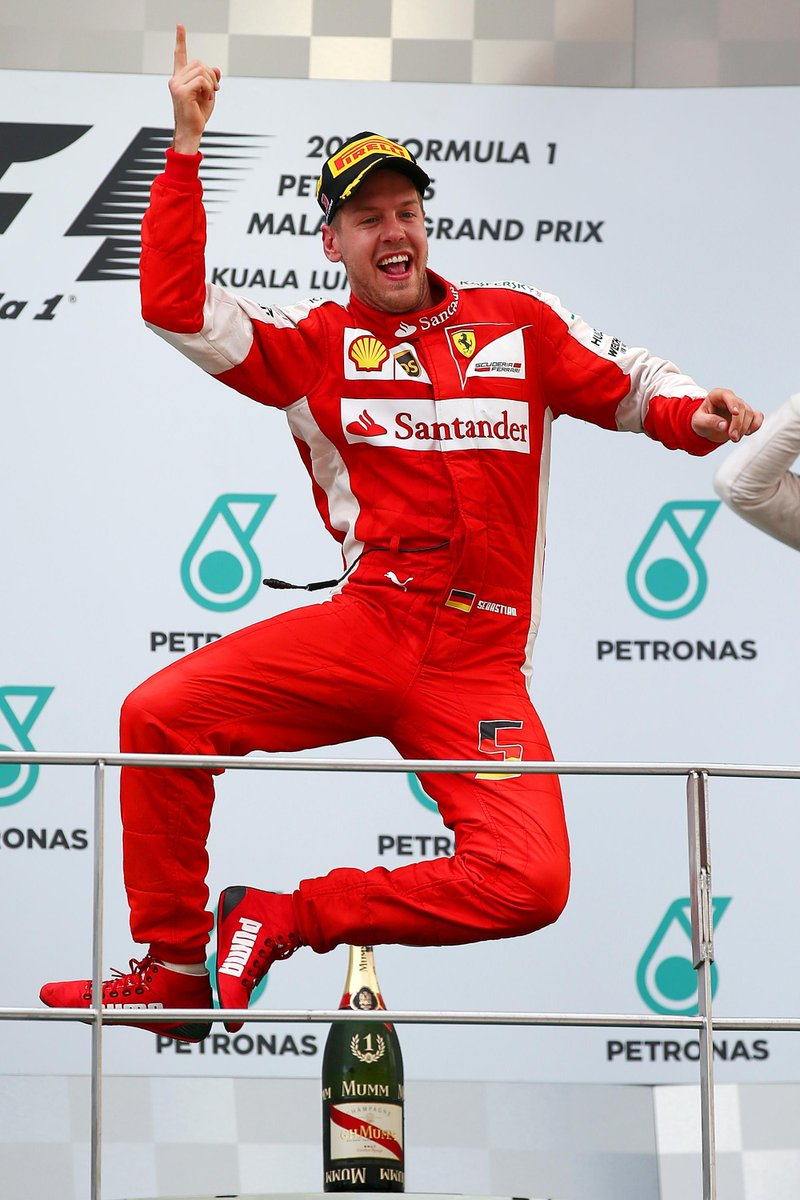
\includegraphics{vettel_dance.jpg}
\caption{CBQQV\_zWQAEr0s2.jpg}
\end{figure}




    % Add a bibliography block to the postdoc
    
    
    
\end{document}
